\chapter{Results}

We make the following measurements at varying:

\begin{itemize}
    \item thickness of Pt and Cu layers; (10 nm, 20 nm, $\ldots$ )
    \item length and width of arm of the \Hst.
\end{itemize}

\label{chapter5}

After making the aforementioned measurements, we proceed to analyze the resultant data.

\begin{figure}[h!]
    \centering
    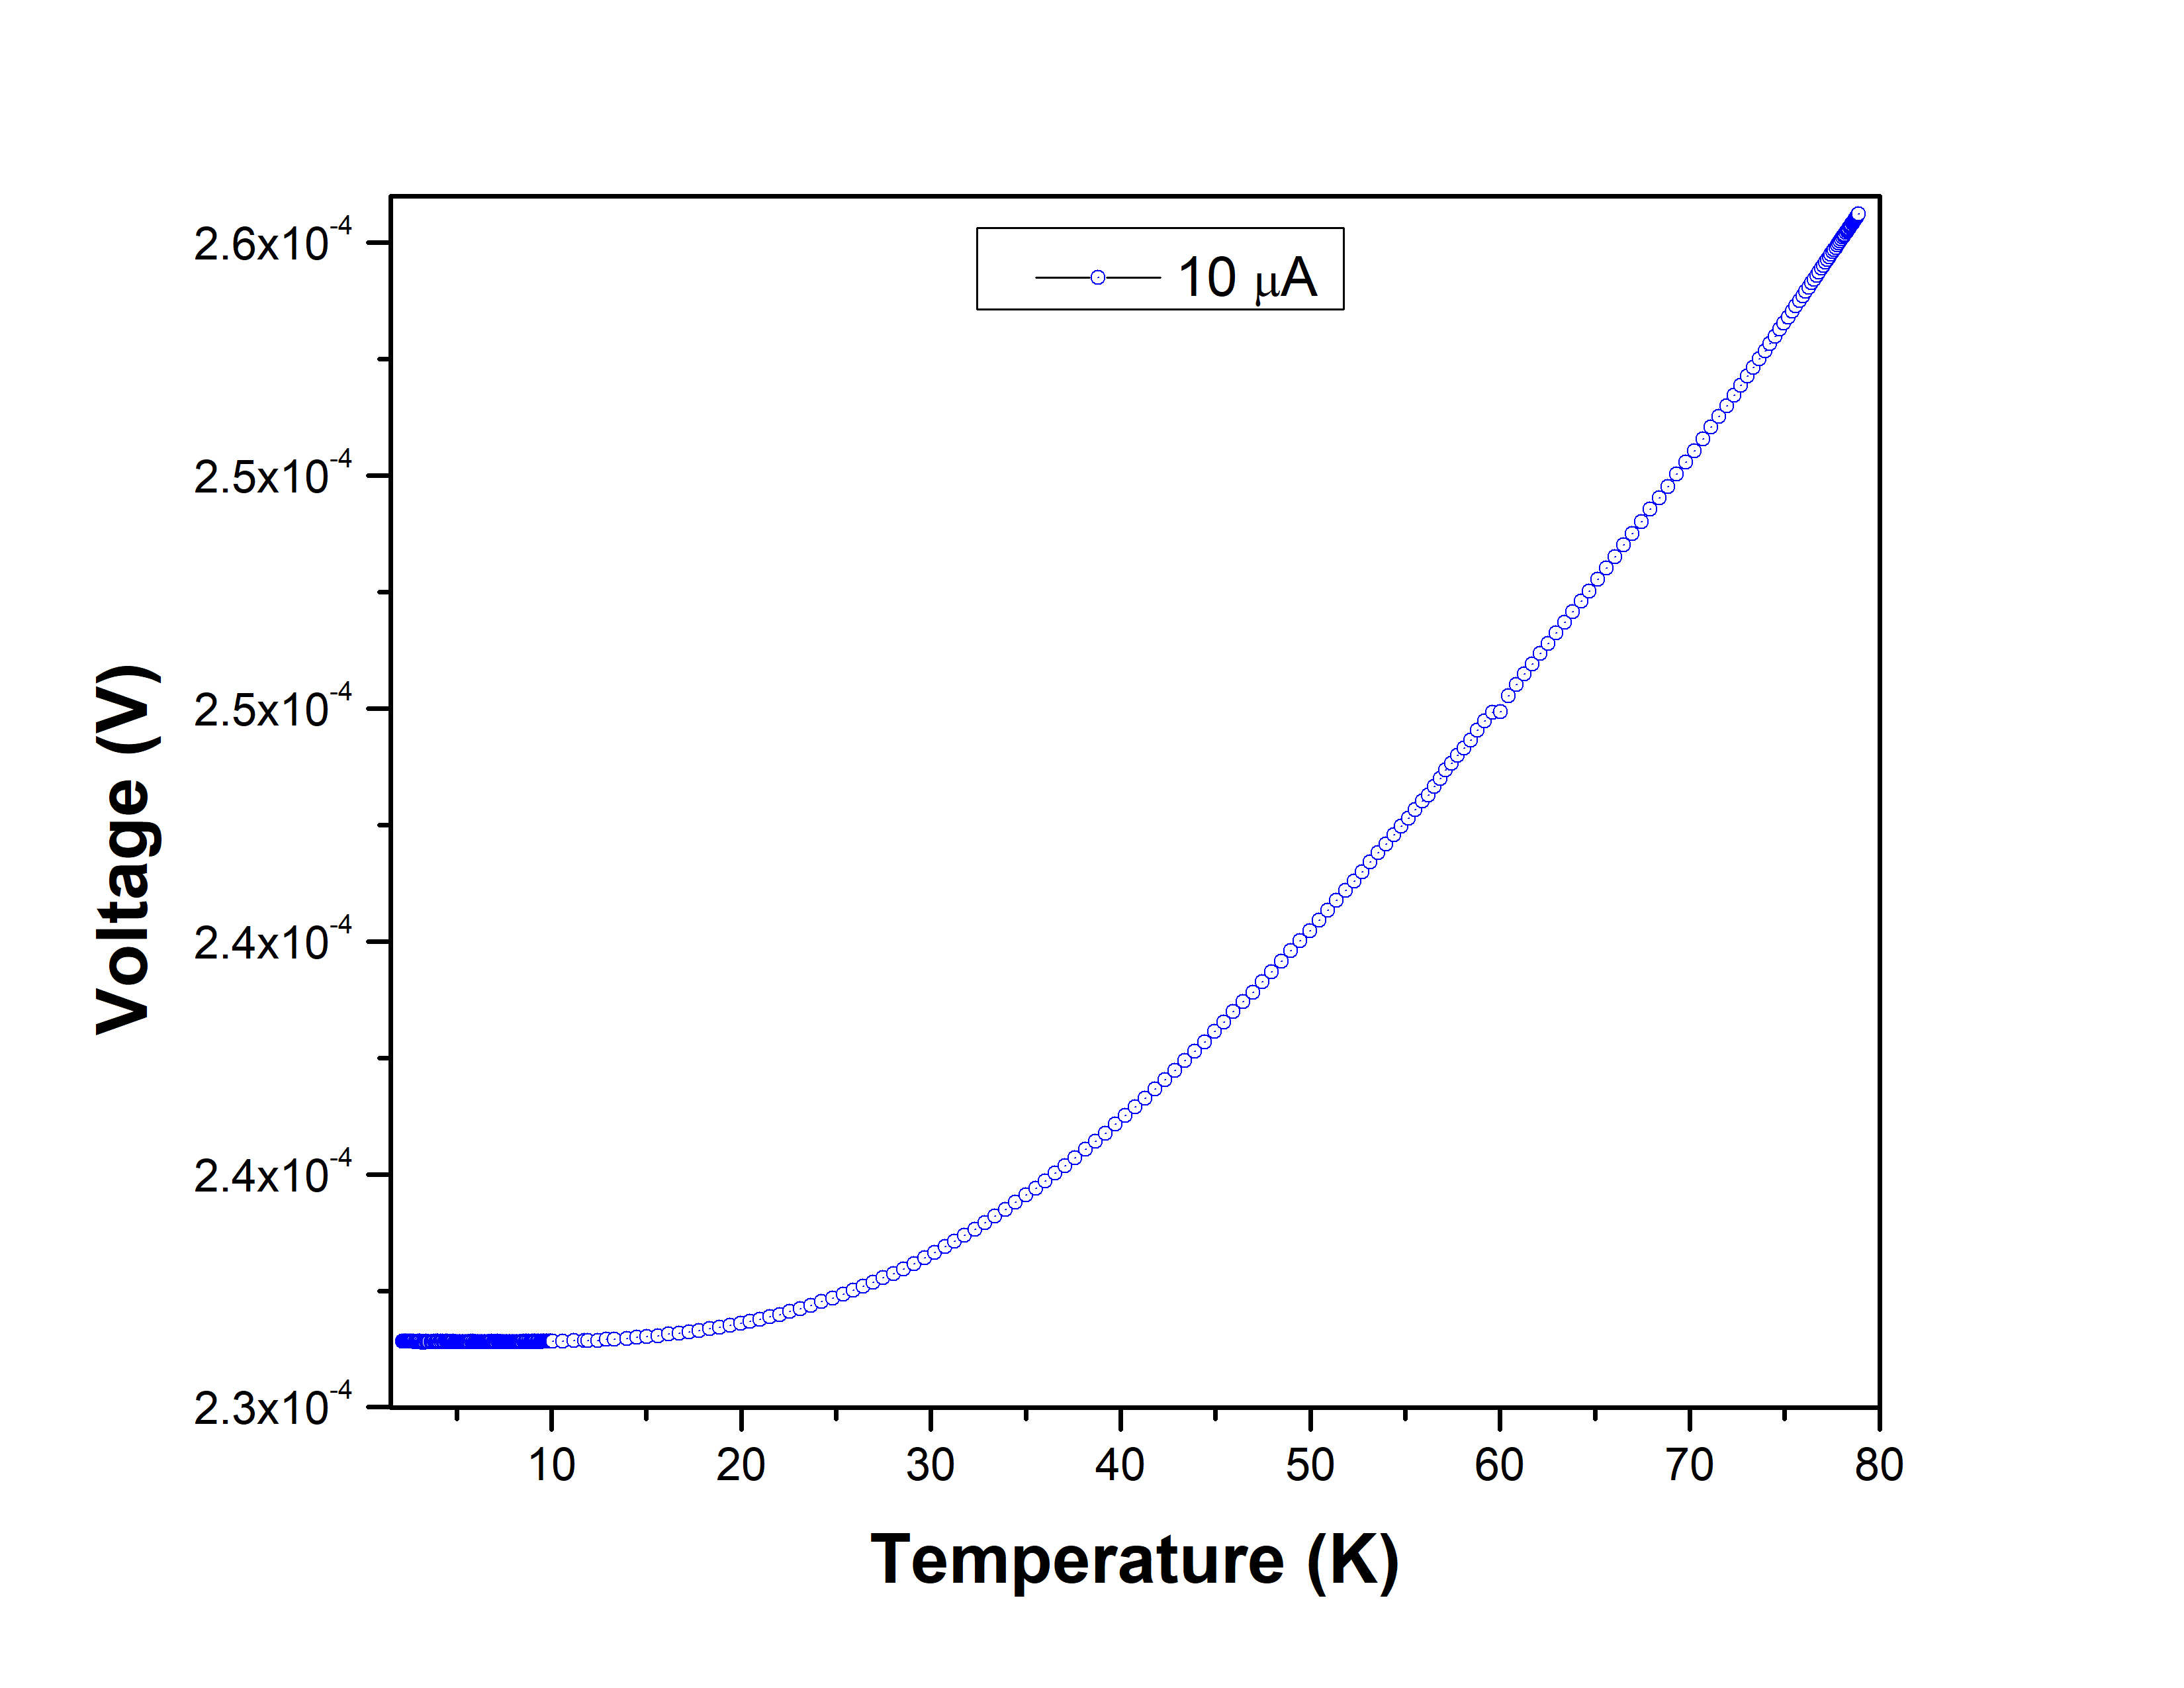
\includegraphics[scale=0.5]{vt-normal1.jpg}
    \caption{Variation of voltage as a function of temperature at constant input current.}
\end{figure}

Before the experiment is begun, we test if the sample track works as one expects.
We supply a fixed value of input current and make voltage measurements at various temperatures of the sample.
As expected, we end up with a \textit{voltage-vs-temperature} curve which is characteristic to that of a metal (Cu/Pt).

\begin{figure}[h!]
    \centering
    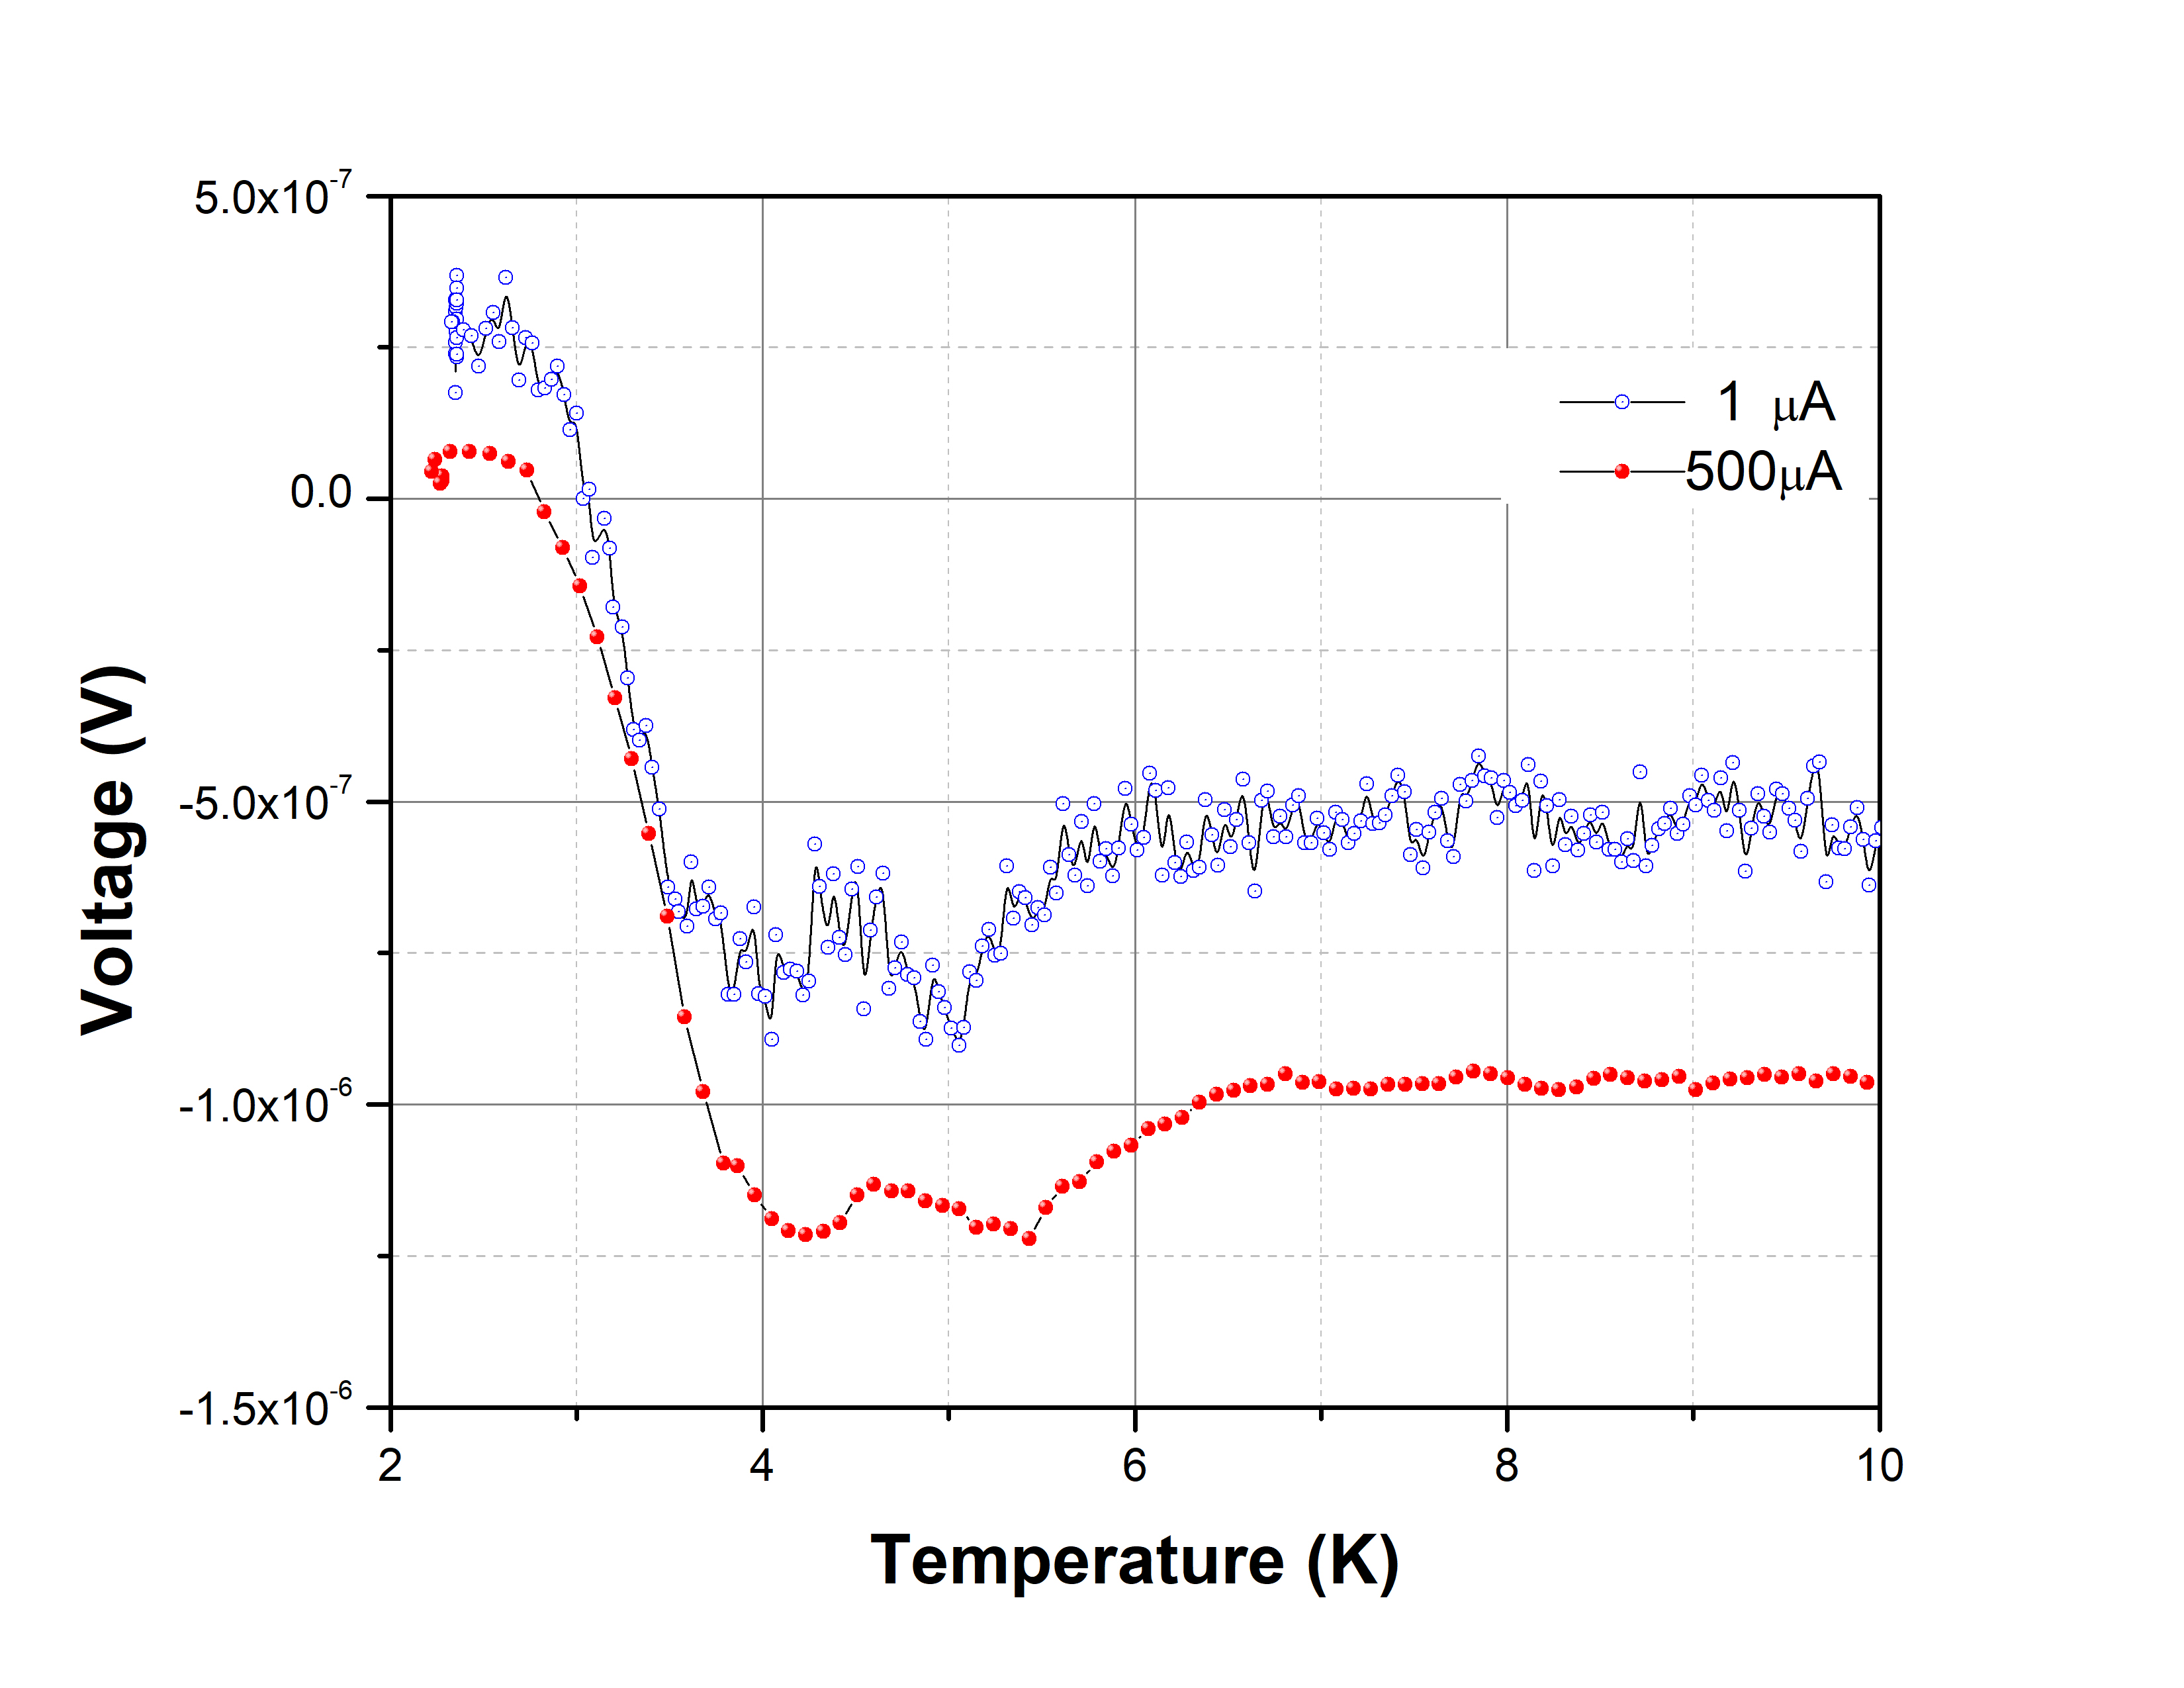
\includegraphics[scale=0.5]{vt.jpg}
    \caption{Variation of voltage for a range of temperature (\( \approx 2 \: K \) to \( 10 \: K \) at constant currents 1 \( \mu \)A and 500 \( \mu \)A).}
    \label{fig:vt}
\end{figure}

On measuring the voltage for a range of temperature (from 2 K to 10 K) at a constant temperature of 1 \( \mu \)A, we see significant noise in \cref{fig:vt} with no particular behaviour. However, doing the same experimental run for a current of 500 \( \mu \)A, we observe a better plot as compared to the case of 1 \( \mu \)A. However, even this plot does not yield any inferable data.

\clearpage

\begin{figure}[h!]
    \centering
    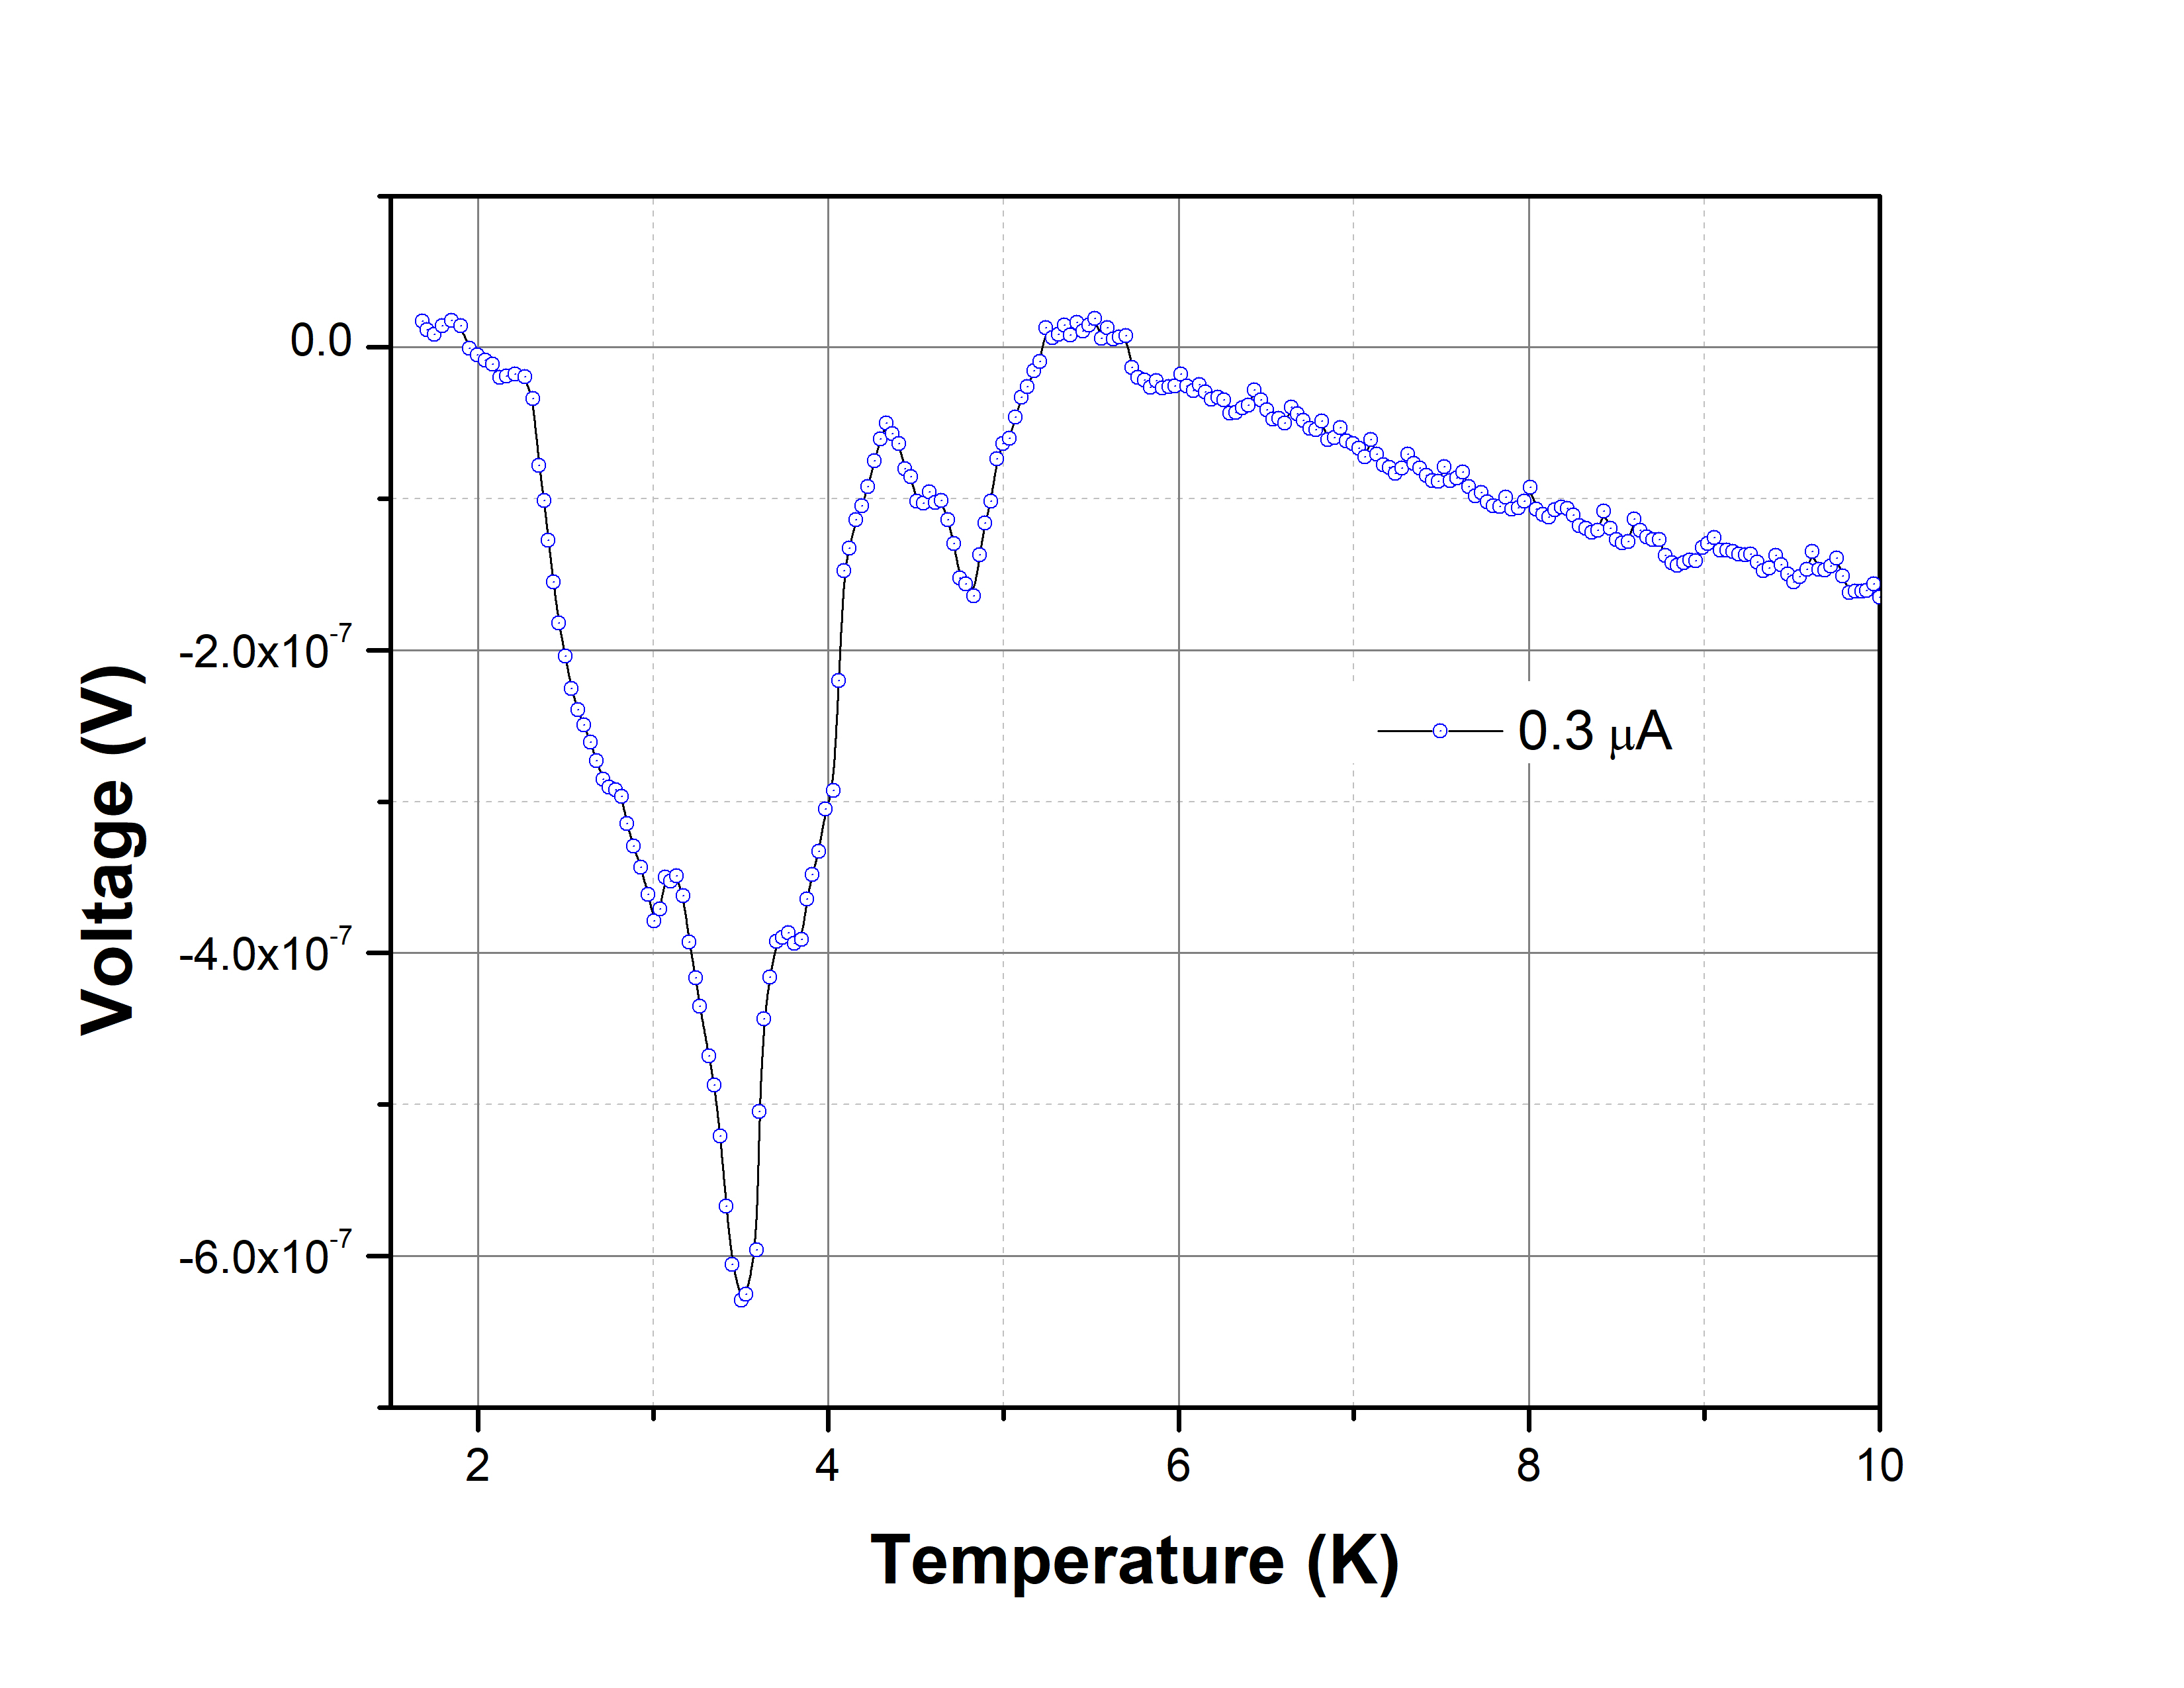
\includegraphics[scale=0.5]{vt-normal.jpg}
    \caption{Testing voltage as a function of temperature against background.}
\end{figure}

To check for if the poor accuracy in plot \ref{fig:vt} is due to stray background potential, we measure it at 0.3 \( \mu \)A, and observe that the variation in voltage shows no correspondence with plot \ref{fig:vt}.

\begin{figure}[h!]
    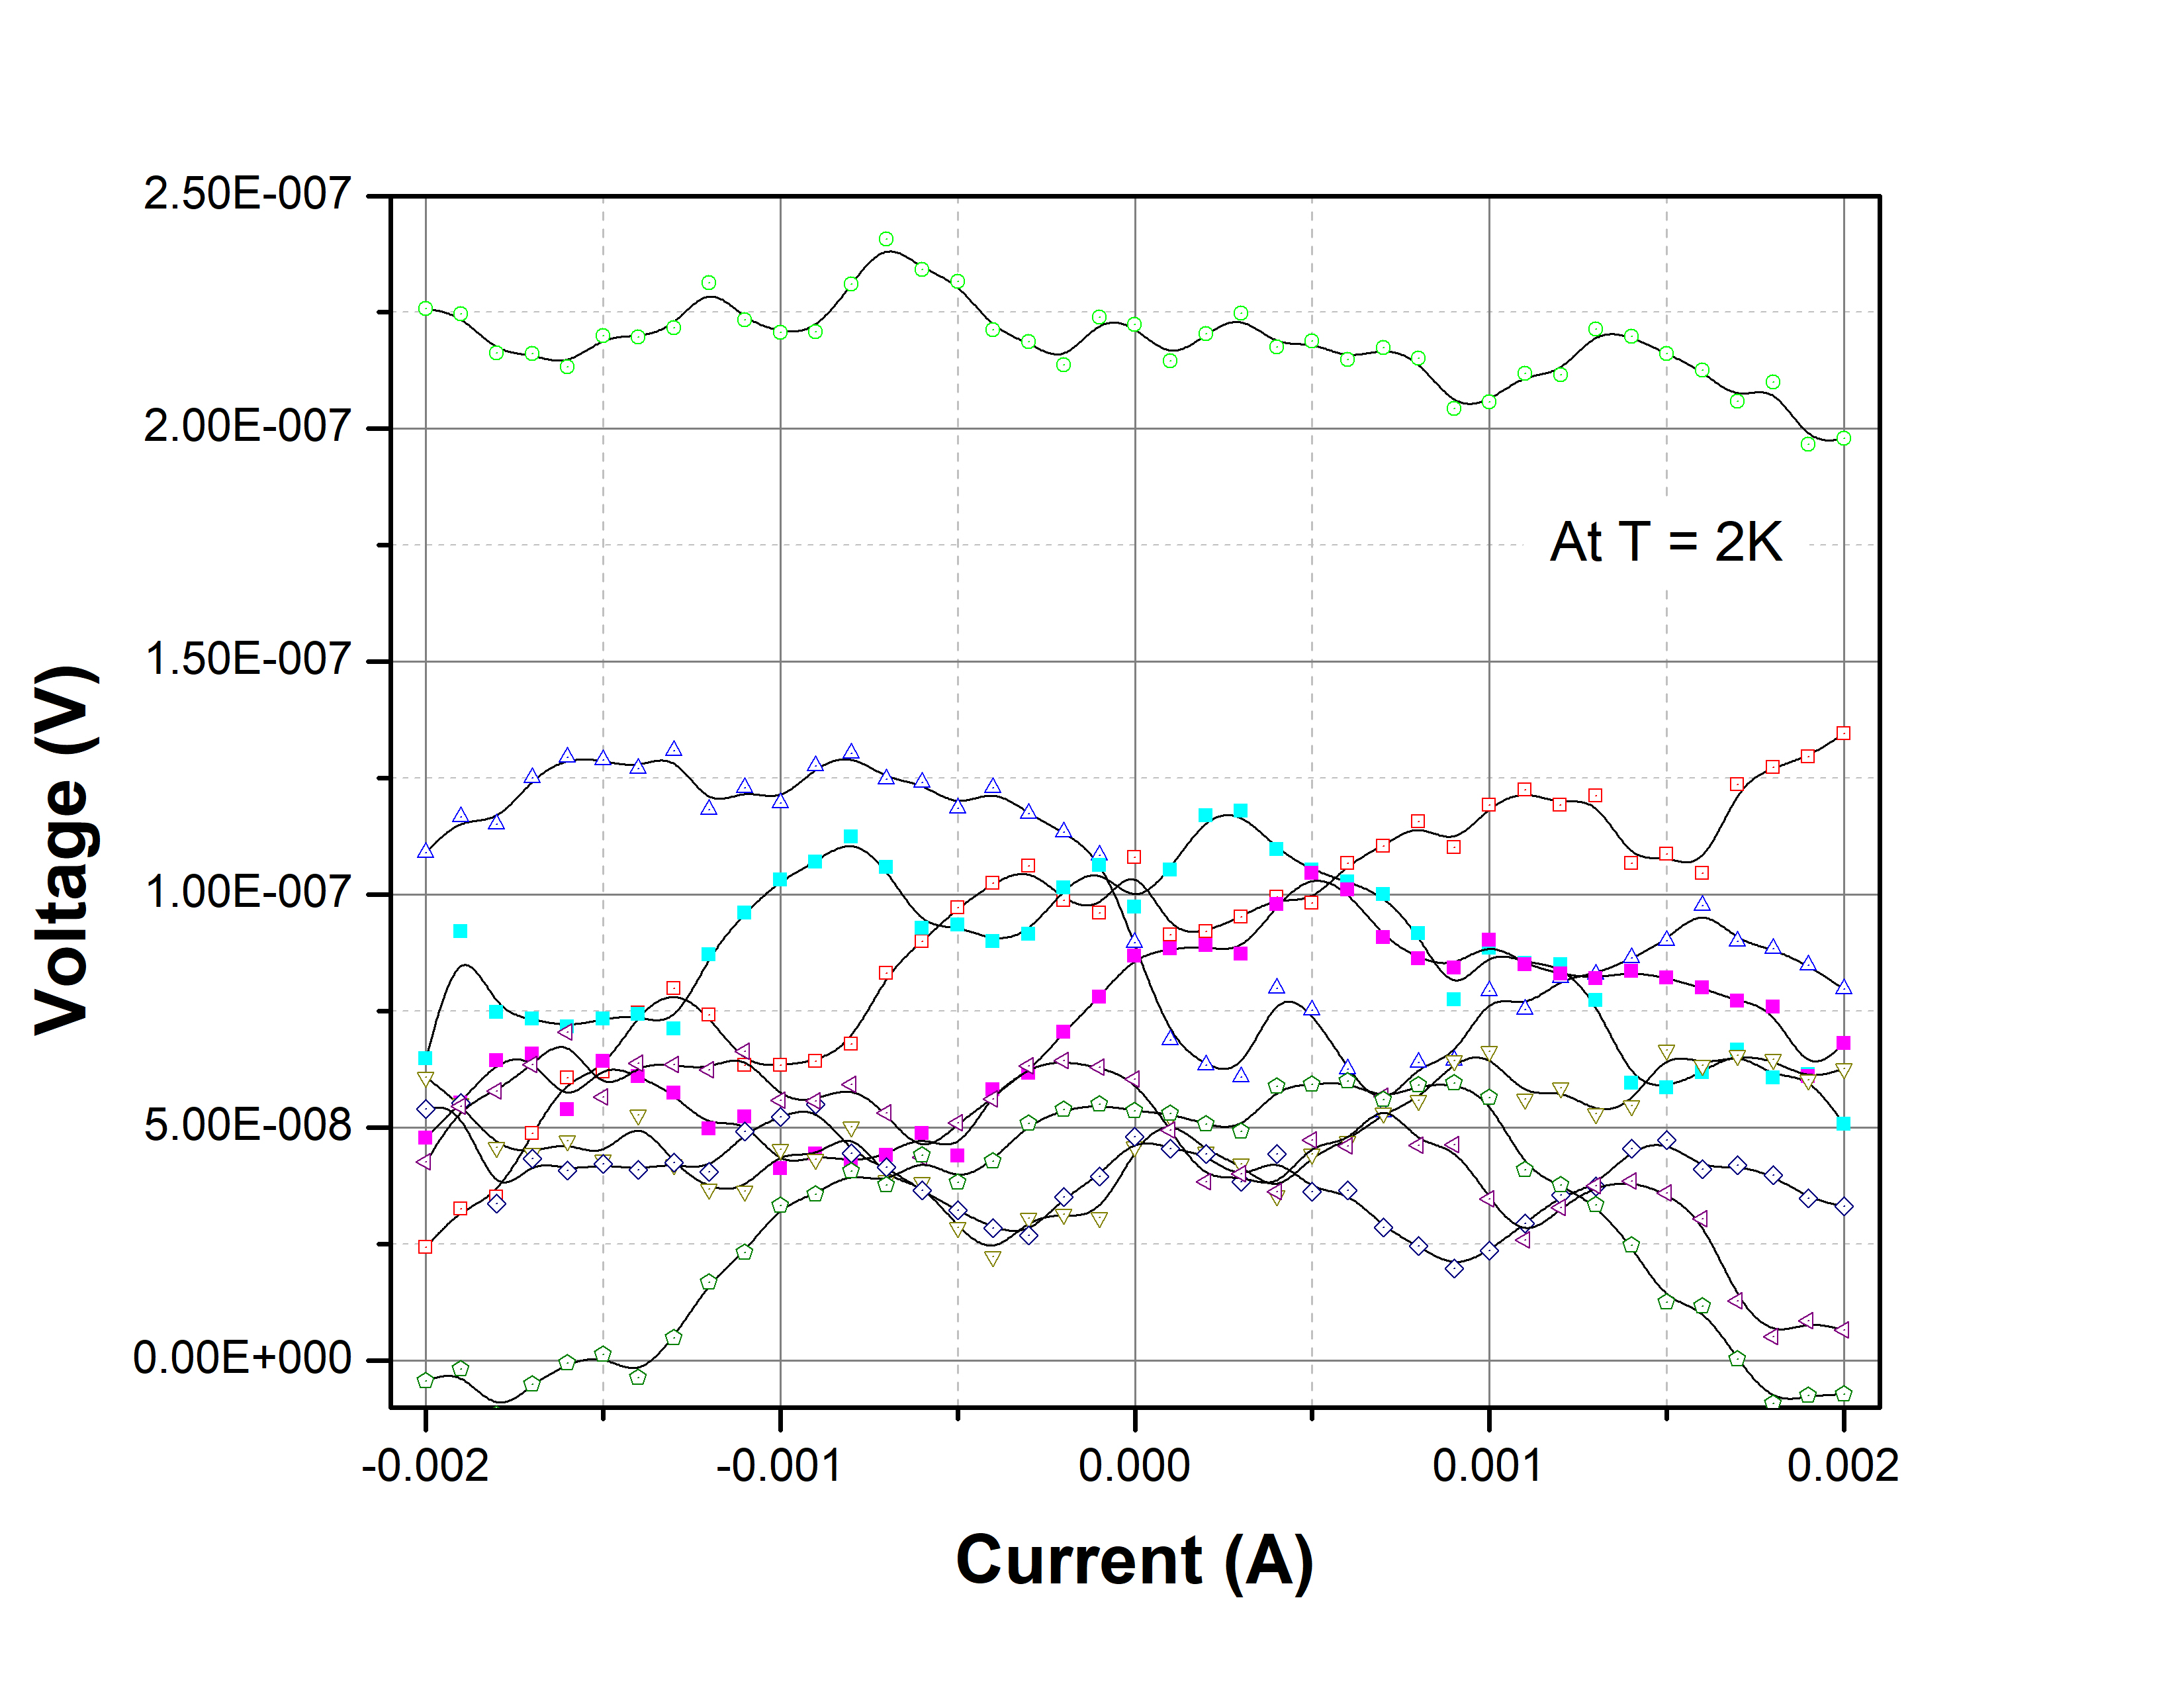
\includegraphics[width=\columnwidth]{vh-compare.jpg}
    \caption{At \( T = 2 \) K, variation of potential difference as input current is varied from -2 mA to +2 mA.}
    \label{fig:vh-compare}
\end{figure}

On varying the input current from -2 mA to +2 mA at a temperature of 2 K, we observe that there is a random variation of non-local voltage measurement in \cref{fig:vh-compare} for a number of runs of the experiment. This unfortunately as well, yields no inferable data.


\clearpage

\subsection{Measurement via extrapolation in the presence of external \( B \) field}

\begin{figure}[!h]
    %% Creator: Matplotlib, PGF backend
%%
%% To include the figure in your LaTeX document, write
%%   \input{<filename>.pgf}
%%
%% Make sure the required packages are loaded in your preamble
%%   \usepackage{pgf}
%%
%% Figures using additional raster images can only be included by \input if
%% they are in the same directory as the main LaTeX file. For loading figures
%% from other directories you can use the `import` package
%%   \usepackage{import}
%%
%% and then include the figures with
%%   \import{<path to file>}{<filename>.pgf}
%%
%% Matplotlib used the following preamble
%%   \usepackage{fontspec}
%%   \setmainfont{DejaVuSerif.ttf}[Path=\detokenize{/usr/lib/python3.9/site-packages/matplotlib/mpl-data/fonts/ttf/}]
%%   \setsansfont{DejaVuSans.ttf}[Path=\detokenize{/usr/lib/python3.9/site-packages/matplotlib/mpl-data/fonts/ttf/}]
%%   \setmonofont{DejaVuSansMono.ttf}[Path=\detokenize{/usr/lib/python3.9/site-packages/matplotlib/mpl-data/fonts/ttf/}]
%%
\begingroup%
\makeatletter%
\begin{pgfpicture}%
\pgfpathrectangle{\pgfpointorigin}{\pgfqpoint{4.919825in}{3.282423in}}%
\pgfusepath{use as bounding box, clip}%
\begin{pgfscope}%
\pgfsetbuttcap%
\pgfsetmiterjoin%
\definecolor{currentfill}{rgb}{1.000000,1.000000,1.000000}%
\pgfsetfillcolor{currentfill}%
\pgfsetlinewidth{0.000000pt}%
\definecolor{currentstroke}{rgb}{1.000000,1.000000,1.000000}%
\pgfsetstrokecolor{currentstroke}%
\pgfsetdash{}{0pt}%
\pgfpathmoveto{\pgfqpoint{0.000000in}{0.000000in}}%
\pgfpathlineto{\pgfqpoint{4.919825in}{0.000000in}}%
\pgfpathlineto{\pgfqpoint{4.919825in}{3.282423in}}%
\pgfpathlineto{\pgfqpoint{0.000000in}{3.282423in}}%
\pgfpathclose%
\pgfusepath{fill}%
\end{pgfscope}%
\begin{pgfscope}%
\pgfsetbuttcap%
\pgfsetmiterjoin%
\definecolor{currentfill}{rgb}{1.000000,1.000000,1.000000}%
\pgfsetfillcolor{currentfill}%
\pgfsetlinewidth{0.000000pt}%
\definecolor{currentstroke}{rgb}{0.000000,0.000000,0.000000}%
\pgfsetstrokecolor{currentstroke}%
\pgfsetstrokeopacity{0.000000}%
\pgfsetdash{}{0pt}%
\pgfpathmoveto{\pgfqpoint{0.537460in}{0.424959in}}%
\pgfpathlineto{\pgfqpoint{4.869825in}{0.424959in}}%
\pgfpathlineto{\pgfqpoint{4.869825in}{3.085233in}}%
\pgfpathlineto{\pgfqpoint{0.537460in}{3.085233in}}%
\pgfpathclose%
\pgfusepath{fill}%
\end{pgfscope}%
\begin{pgfscope}%
\pgfsetbuttcap%
\pgfsetroundjoin%
\definecolor{currentfill}{rgb}{0.000000,0.000000,0.000000}%
\pgfsetfillcolor{currentfill}%
\pgfsetlinewidth{0.501875pt}%
\definecolor{currentstroke}{rgb}{0.000000,0.000000,0.000000}%
\pgfsetstrokecolor{currentstroke}%
\pgfsetdash{}{0pt}%
\pgfsys@defobject{currentmarker}{\pgfqpoint{0.000000in}{0.000000in}}{\pgfqpoint{0.000000in}{0.041667in}}{%
\pgfpathmoveto{\pgfqpoint{0.000000in}{0.000000in}}%
\pgfpathlineto{\pgfqpoint{0.000000in}{0.041667in}}%
\pgfusepath{stroke,fill}%
}%
\begin{pgfscope}%
\pgfsys@transformshift{0.734386in}{0.424959in}%
\pgfsys@useobject{currentmarker}{}%
\end{pgfscope}%
\end{pgfscope}%
\begin{pgfscope}%
\pgfsetbuttcap%
\pgfsetroundjoin%
\definecolor{currentfill}{rgb}{0.000000,0.000000,0.000000}%
\pgfsetfillcolor{currentfill}%
\pgfsetlinewidth{0.501875pt}%
\definecolor{currentstroke}{rgb}{0.000000,0.000000,0.000000}%
\pgfsetstrokecolor{currentstroke}%
\pgfsetdash{}{0pt}%
\pgfsys@defobject{currentmarker}{\pgfqpoint{0.000000in}{-0.041667in}}{\pgfqpoint{0.000000in}{0.000000in}}{%
\pgfpathmoveto{\pgfqpoint{0.000000in}{0.000000in}}%
\pgfpathlineto{\pgfqpoint{0.000000in}{-0.041667in}}%
\pgfusepath{stroke,fill}%
}%
\begin{pgfscope}%
\pgfsys@transformshift{0.734386in}{3.085233in}%
\pgfsys@useobject{currentmarker}{}%
\end{pgfscope}%
\end{pgfscope}%
\begin{pgfscope}%
\definecolor{textcolor}{rgb}{0.000000,0.000000,0.000000}%
\pgfsetstrokecolor{textcolor}%
\pgfsetfillcolor{textcolor}%
\pgftext[x=0.734386in,y=0.376348in,,top]{\color{textcolor}\rmfamily\fontsize{10.000000}{12.000000}\selectfont \(\displaystyle {0}\)}%
\end{pgfscope}%
\begin{pgfscope}%
\pgfsetbuttcap%
\pgfsetroundjoin%
\definecolor{currentfill}{rgb}{0.000000,0.000000,0.000000}%
\pgfsetfillcolor{currentfill}%
\pgfsetlinewidth{0.501875pt}%
\definecolor{currentstroke}{rgb}{0.000000,0.000000,0.000000}%
\pgfsetstrokecolor{currentstroke}%
\pgfsetdash{}{0pt}%
\pgfsys@defobject{currentmarker}{\pgfqpoint{0.000000in}{0.000000in}}{\pgfqpoint{0.000000in}{0.041667in}}{%
\pgfpathmoveto{\pgfqpoint{0.000000in}{0.000000in}}%
\pgfpathlineto{\pgfqpoint{0.000000in}{0.041667in}}%
\pgfusepath{stroke,fill}%
}%
\begin{pgfscope}%
\pgfsys@transformshift{1.390816in}{0.424959in}%
\pgfsys@useobject{currentmarker}{}%
\end{pgfscope}%
\end{pgfscope}%
\begin{pgfscope}%
\pgfsetbuttcap%
\pgfsetroundjoin%
\definecolor{currentfill}{rgb}{0.000000,0.000000,0.000000}%
\pgfsetfillcolor{currentfill}%
\pgfsetlinewidth{0.501875pt}%
\definecolor{currentstroke}{rgb}{0.000000,0.000000,0.000000}%
\pgfsetstrokecolor{currentstroke}%
\pgfsetdash{}{0pt}%
\pgfsys@defobject{currentmarker}{\pgfqpoint{0.000000in}{-0.041667in}}{\pgfqpoint{0.000000in}{0.000000in}}{%
\pgfpathmoveto{\pgfqpoint{0.000000in}{0.000000in}}%
\pgfpathlineto{\pgfqpoint{0.000000in}{-0.041667in}}%
\pgfusepath{stroke,fill}%
}%
\begin{pgfscope}%
\pgfsys@transformshift{1.390816in}{3.085233in}%
\pgfsys@useobject{currentmarker}{}%
\end{pgfscope}%
\end{pgfscope}%
\begin{pgfscope}%
\definecolor{textcolor}{rgb}{0.000000,0.000000,0.000000}%
\pgfsetstrokecolor{textcolor}%
\pgfsetfillcolor{textcolor}%
\pgftext[x=1.390816in,y=0.376348in,,top]{\color{textcolor}\rmfamily\fontsize{10.000000}{12.000000}\selectfont \(\displaystyle {1}\)}%
\end{pgfscope}%
\begin{pgfscope}%
\pgfsetbuttcap%
\pgfsetroundjoin%
\definecolor{currentfill}{rgb}{0.000000,0.000000,0.000000}%
\pgfsetfillcolor{currentfill}%
\pgfsetlinewidth{0.501875pt}%
\definecolor{currentstroke}{rgb}{0.000000,0.000000,0.000000}%
\pgfsetstrokecolor{currentstroke}%
\pgfsetdash{}{0pt}%
\pgfsys@defobject{currentmarker}{\pgfqpoint{0.000000in}{0.000000in}}{\pgfqpoint{0.000000in}{0.041667in}}{%
\pgfpathmoveto{\pgfqpoint{0.000000in}{0.000000in}}%
\pgfpathlineto{\pgfqpoint{0.000000in}{0.041667in}}%
\pgfusepath{stroke,fill}%
}%
\begin{pgfscope}%
\pgfsys@transformshift{2.047246in}{0.424959in}%
\pgfsys@useobject{currentmarker}{}%
\end{pgfscope}%
\end{pgfscope}%
\begin{pgfscope}%
\pgfsetbuttcap%
\pgfsetroundjoin%
\definecolor{currentfill}{rgb}{0.000000,0.000000,0.000000}%
\pgfsetfillcolor{currentfill}%
\pgfsetlinewidth{0.501875pt}%
\definecolor{currentstroke}{rgb}{0.000000,0.000000,0.000000}%
\pgfsetstrokecolor{currentstroke}%
\pgfsetdash{}{0pt}%
\pgfsys@defobject{currentmarker}{\pgfqpoint{0.000000in}{-0.041667in}}{\pgfqpoint{0.000000in}{0.000000in}}{%
\pgfpathmoveto{\pgfqpoint{0.000000in}{0.000000in}}%
\pgfpathlineto{\pgfqpoint{0.000000in}{-0.041667in}}%
\pgfusepath{stroke,fill}%
}%
\begin{pgfscope}%
\pgfsys@transformshift{2.047246in}{3.085233in}%
\pgfsys@useobject{currentmarker}{}%
\end{pgfscope}%
\end{pgfscope}%
\begin{pgfscope}%
\definecolor{textcolor}{rgb}{0.000000,0.000000,0.000000}%
\pgfsetstrokecolor{textcolor}%
\pgfsetfillcolor{textcolor}%
\pgftext[x=2.047246in,y=0.376348in,,top]{\color{textcolor}\rmfamily\fontsize{10.000000}{12.000000}\selectfont \(\displaystyle {2}\)}%
\end{pgfscope}%
\begin{pgfscope}%
\pgfsetbuttcap%
\pgfsetroundjoin%
\definecolor{currentfill}{rgb}{0.000000,0.000000,0.000000}%
\pgfsetfillcolor{currentfill}%
\pgfsetlinewidth{0.501875pt}%
\definecolor{currentstroke}{rgb}{0.000000,0.000000,0.000000}%
\pgfsetstrokecolor{currentstroke}%
\pgfsetdash{}{0pt}%
\pgfsys@defobject{currentmarker}{\pgfqpoint{0.000000in}{0.000000in}}{\pgfqpoint{0.000000in}{0.041667in}}{%
\pgfpathmoveto{\pgfqpoint{0.000000in}{0.000000in}}%
\pgfpathlineto{\pgfqpoint{0.000000in}{0.041667in}}%
\pgfusepath{stroke,fill}%
}%
\begin{pgfscope}%
\pgfsys@transformshift{2.703676in}{0.424959in}%
\pgfsys@useobject{currentmarker}{}%
\end{pgfscope}%
\end{pgfscope}%
\begin{pgfscope}%
\pgfsetbuttcap%
\pgfsetroundjoin%
\definecolor{currentfill}{rgb}{0.000000,0.000000,0.000000}%
\pgfsetfillcolor{currentfill}%
\pgfsetlinewidth{0.501875pt}%
\definecolor{currentstroke}{rgb}{0.000000,0.000000,0.000000}%
\pgfsetstrokecolor{currentstroke}%
\pgfsetdash{}{0pt}%
\pgfsys@defobject{currentmarker}{\pgfqpoint{0.000000in}{-0.041667in}}{\pgfqpoint{0.000000in}{0.000000in}}{%
\pgfpathmoveto{\pgfqpoint{0.000000in}{0.000000in}}%
\pgfpathlineto{\pgfqpoint{0.000000in}{-0.041667in}}%
\pgfusepath{stroke,fill}%
}%
\begin{pgfscope}%
\pgfsys@transformshift{2.703676in}{3.085233in}%
\pgfsys@useobject{currentmarker}{}%
\end{pgfscope}%
\end{pgfscope}%
\begin{pgfscope}%
\definecolor{textcolor}{rgb}{0.000000,0.000000,0.000000}%
\pgfsetstrokecolor{textcolor}%
\pgfsetfillcolor{textcolor}%
\pgftext[x=2.703676in,y=0.376348in,,top]{\color{textcolor}\rmfamily\fontsize{10.000000}{12.000000}\selectfont \(\displaystyle {3}\)}%
\end{pgfscope}%
\begin{pgfscope}%
\pgfsetbuttcap%
\pgfsetroundjoin%
\definecolor{currentfill}{rgb}{0.000000,0.000000,0.000000}%
\pgfsetfillcolor{currentfill}%
\pgfsetlinewidth{0.501875pt}%
\definecolor{currentstroke}{rgb}{0.000000,0.000000,0.000000}%
\pgfsetstrokecolor{currentstroke}%
\pgfsetdash{}{0pt}%
\pgfsys@defobject{currentmarker}{\pgfqpoint{0.000000in}{0.000000in}}{\pgfqpoint{0.000000in}{0.041667in}}{%
\pgfpathmoveto{\pgfqpoint{0.000000in}{0.000000in}}%
\pgfpathlineto{\pgfqpoint{0.000000in}{0.041667in}}%
\pgfusepath{stroke,fill}%
}%
\begin{pgfscope}%
\pgfsys@transformshift{3.360105in}{0.424959in}%
\pgfsys@useobject{currentmarker}{}%
\end{pgfscope}%
\end{pgfscope}%
\begin{pgfscope}%
\pgfsetbuttcap%
\pgfsetroundjoin%
\definecolor{currentfill}{rgb}{0.000000,0.000000,0.000000}%
\pgfsetfillcolor{currentfill}%
\pgfsetlinewidth{0.501875pt}%
\definecolor{currentstroke}{rgb}{0.000000,0.000000,0.000000}%
\pgfsetstrokecolor{currentstroke}%
\pgfsetdash{}{0pt}%
\pgfsys@defobject{currentmarker}{\pgfqpoint{0.000000in}{-0.041667in}}{\pgfqpoint{0.000000in}{0.000000in}}{%
\pgfpathmoveto{\pgfqpoint{0.000000in}{0.000000in}}%
\pgfpathlineto{\pgfqpoint{0.000000in}{-0.041667in}}%
\pgfusepath{stroke,fill}%
}%
\begin{pgfscope}%
\pgfsys@transformshift{3.360105in}{3.085233in}%
\pgfsys@useobject{currentmarker}{}%
\end{pgfscope}%
\end{pgfscope}%
\begin{pgfscope}%
\definecolor{textcolor}{rgb}{0.000000,0.000000,0.000000}%
\pgfsetstrokecolor{textcolor}%
\pgfsetfillcolor{textcolor}%
\pgftext[x=3.360105in,y=0.376348in,,top]{\color{textcolor}\rmfamily\fontsize{10.000000}{12.000000}\selectfont \(\displaystyle {4}\)}%
\end{pgfscope}%
\begin{pgfscope}%
\pgfsetbuttcap%
\pgfsetroundjoin%
\definecolor{currentfill}{rgb}{0.000000,0.000000,0.000000}%
\pgfsetfillcolor{currentfill}%
\pgfsetlinewidth{0.501875pt}%
\definecolor{currentstroke}{rgb}{0.000000,0.000000,0.000000}%
\pgfsetstrokecolor{currentstroke}%
\pgfsetdash{}{0pt}%
\pgfsys@defobject{currentmarker}{\pgfqpoint{0.000000in}{0.000000in}}{\pgfqpoint{0.000000in}{0.041667in}}{%
\pgfpathmoveto{\pgfqpoint{0.000000in}{0.000000in}}%
\pgfpathlineto{\pgfqpoint{0.000000in}{0.041667in}}%
\pgfusepath{stroke,fill}%
}%
\begin{pgfscope}%
\pgfsys@transformshift{4.016535in}{0.424959in}%
\pgfsys@useobject{currentmarker}{}%
\end{pgfscope}%
\end{pgfscope}%
\begin{pgfscope}%
\pgfsetbuttcap%
\pgfsetroundjoin%
\definecolor{currentfill}{rgb}{0.000000,0.000000,0.000000}%
\pgfsetfillcolor{currentfill}%
\pgfsetlinewidth{0.501875pt}%
\definecolor{currentstroke}{rgb}{0.000000,0.000000,0.000000}%
\pgfsetstrokecolor{currentstroke}%
\pgfsetdash{}{0pt}%
\pgfsys@defobject{currentmarker}{\pgfqpoint{0.000000in}{-0.041667in}}{\pgfqpoint{0.000000in}{0.000000in}}{%
\pgfpathmoveto{\pgfqpoint{0.000000in}{0.000000in}}%
\pgfpathlineto{\pgfqpoint{0.000000in}{-0.041667in}}%
\pgfusepath{stroke,fill}%
}%
\begin{pgfscope}%
\pgfsys@transformshift{4.016535in}{3.085233in}%
\pgfsys@useobject{currentmarker}{}%
\end{pgfscope}%
\end{pgfscope}%
\begin{pgfscope}%
\definecolor{textcolor}{rgb}{0.000000,0.000000,0.000000}%
\pgfsetstrokecolor{textcolor}%
\pgfsetfillcolor{textcolor}%
\pgftext[x=4.016535in,y=0.376348in,,top]{\color{textcolor}\rmfamily\fontsize{10.000000}{12.000000}\selectfont \(\displaystyle {5}\)}%
\end{pgfscope}%
\begin{pgfscope}%
\pgfsetbuttcap%
\pgfsetroundjoin%
\definecolor{currentfill}{rgb}{0.000000,0.000000,0.000000}%
\pgfsetfillcolor{currentfill}%
\pgfsetlinewidth{0.501875pt}%
\definecolor{currentstroke}{rgb}{0.000000,0.000000,0.000000}%
\pgfsetstrokecolor{currentstroke}%
\pgfsetdash{}{0pt}%
\pgfsys@defobject{currentmarker}{\pgfqpoint{0.000000in}{0.000000in}}{\pgfqpoint{0.000000in}{0.041667in}}{%
\pgfpathmoveto{\pgfqpoint{0.000000in}{0.000000in}}%
\pgfpathlineto{\pgfqpoint{0.000000in}{0.041667in}}%
\pgfusepath{stroke,fill}%
}%
\begin{pgfscope}%
\pgfsys@transformshift{4.672965in}{0.424959in}%
\pgfsys@useobject{currentmarker}{}%
\end{pgfscope}%
\end{pgfscope}%
\begin{pgfscope}%
\pgfsetbuttcap%
\pgfsetroundjoin%
\definecolor{currentfill}{rgb}{0.000000,0.000000,0.000000}%
\pgfsetfillcolor{currentfill}%
\pgfsetlinewidth{0.501875pt}%
\definecolor{currentstroke}{rgb}{0.000000,0.000000,0.000000}%
\pgfsetstrokecolor{currentstroke}%
\pgfsetdash{}{0pt}%
\pgfsys@defobject{currentmarker}{\pgfqpoint{0.000000in}{-0.041667in}}{\pgfqpoint{0.000000in}{0.000000in}}{%
\pgfpathmoveto{\pgfqpoint{0.000000in}{0.000000in}}%
\pgfpathlineto{\pgfqpoint{0.000000in}{-0.041667in}}%
\pgfusepath{stroke,fill}%
}%
\begin{pgfscope}%
\pgfsys@transformshift{4.672965in}{3.085233in}%
\pgfsys@useobject{currentmarker}{}%
\end{pgfscope}%
\end{pgfscope}%
\begin{pgfscope}%
\definecolor{textcolor}{rgb}{0.000000,0.000000,0.000000}%
\pgfsetstrokecolor{textcolor}%
\pgfsetfillcolor{textcolor}%
\pgftext[x=4.672965in,y=0.376348in,,top]{\color{textcolor}\rmfamily\fontsize{10.000000}{12.000000}\selectfont \(\displaystyle {6}\)}%
\end{pgfscope}%
\begin{pgfscope}%
\pgfsetbuttcap%
\pgfsetroundjoin%
\definecolor{currentfill}{rgb}{0.000000,0.000000,0.000000}%
\pgfsetfillcolor{currentfill}%
\pgfsetlinewidth{0.501875pt}%
\definecolor{currentstroke}{rgb}{0.000000,0.000000,0.000000}%
\pgfsetstrokecolor{currentstroke}%
\pgfsetdash{}{0pt}%
\pgfsys@defobject{currentmarker}{\pgfqpoint{0.000000in}{0.000000in}}{\pgfqpoint{0.000000in}{0.020833in}}{%
\pgfpathmoveto{\pgfqpoint{0.000000in}{0.000000in}}%
\pgfpathlineto{\pgfqpoint{0.000000in}{0.020833in}}%
\pgfusepath{stroke,fill}%
}%
\begin{pgfscope}%
\pgfsys@transformshift{0.603100in}{0.424959in}%
\pgfsys@useobject{currentmarker}{}%
\end{pgfscope}%
\end{pgfscope}%
\begin{pgfscope}%
\pgfsetbuttcap%
\pgfsetroundjoin%
\definecolor{currentfill}{rgb}{0.000000,0.000000,0.000000}%
\pgfsetfillcolor{currentfill}%
\pgfsetlinewidth{0.501875pt}%
\definecolor{currentstroke}{rgb}{0.000000,0.000000,0.000000}%
\pgfsetstrokecolor{currentstroke}%
\pgfsetdash{}{0pt}%
\pgfsys@defobject{currentmarker}{\pgfqpoint{0.000000in}{-0.020833in}}{\pgfqpoint{0.000000in}{0.000000in}}{%
\pgfpathmoveto{\pgfqpoint{0.000000in}{0.000000in}}%
\pgfpathlineto{\pgfqpoint{0.000000in}{-0.020833in}}%
\pgfusepath{stroke,fill}%
}%
\begin{pgfscope}%
\pgfsys@transformshift{0.603100in}{3.085233in}%
\pgfsys@useobject{currentmarker}{}%
\end{pgfscope}%
\end{pgfscope}%
\begin{pgfscope}%
\pgfsetbuttcap%
\pgfsetroundjoin%
\definecolor{currentfill}{rgb}{0.000000,0.000000,0.000000}%
\pgfsetfillcolor{currentfill}%
\pgfsetlinewidth{0.501875pt}%
\definecolor{currentstroke}{rgb}{0.000000,0.000000,0.000000}%
\pgfsetstrokecolor{currentstroke}%
\pgfsetdash{}{0pt}%
\pgfsys@defobject{currentmarker}{\pgfqpoint{0.000000in}{0.000000in}}{\pgfqpoint{0.000000in}{0.020833in}}{%
\pgfpathmoveto{\pgfqpoint{0.000000in}{0.000000in}}%
\pgfpathlineto{\pgfqpoint{0.000000in}{0.020833in}}%
\pgfusepath{stroke,fill}%
}%
\begin{pgfscope}%
\pgfsys@transformshift{0.865672in}{0.424959in}%
\pgfsys@useobject{currentmarker}{}%
\end{pgfscope}%
\end{pgfscope}%
\begin{pgfscope}%
\pgfsetbuttcap%
\pgfsetroundjoin%
\definecolor{currentfill}{rgb}{0.000000,0.000000,0.000000}%
\pgfsetfillcolor{currentfill}%
\pgfsetlinewidth{0.501875pt}%
\definecolor{currentstroke}{rgb}{0.000000,0.000000,0.000000}%
\pgfsetstrokecolor{currentstroke}%
\pgfsetdash{}{0pt}%
\pgfsys@defobject{currentmarker}{\pgfqpoint{0.000000in}{-0.020833in}}{\pgfqpoint{0.000000in}{0.000000in}}{%
\pgfpathmoveto{\pgfqpoint{0.000000in}{0.000000in}}%
\pgfpathlineto{\pgfqpoint{0.000000in}{-0.020833in}}%
\pgfusepath{stroke,fill}%
}%
\begin{pgfscope}%
\pgfsys@transformshift{0.865672in}{3.085233in}%
\pgfsys@useobject{currentmarker}{}%
\end{pgfscope}%
\end{pgfscope}%
\begin{pgfscope}%
\pgfsetbuttcap%
\pgfsetroundjoin%
\definecolor{currentfill}{rgb}{0.000000,0.000000,0.000000}%
\pgfsetfillcolor{currentfill}%
\pgfsetlinewidth{0.501875pt}%
\definecolor{currentstroke}{rgb}{0.000000,0.000000,0.000000}%
\pgfsetstrokecolor{currentstroke}%
\pgfsetdash{}{0pt}%
\pgfsys@defobject{currentmarker}{\pgfqpoint{0.000000in}{0.000000in}}{\pgfqpoint{0.000000in}{0.020833in}}{%
\pgfpathmoveto{\pgfqpoint{0.000000in}{0.000000in}}%
\pgfpathlineto{\pgfqpoint{0.000000in}{0.020833in}}%
\pgfusepath{stroke,fill}%
}%
\begin{pgfscope}%
\pgfsys@transformshift{0.996958in}{0.424959in}%
\pgfsys@useobject{currentmarker}{}%
\end{pgfscope}%
\end{pgfscope}%
\begin{pgfscope}%
\pgfsetbuttcap%
\pgfsetroundjoin%
\definecolor{currentfill}{rgb}{0.000000,0.000000,0.000000}%
\pgfsetfillcolor{currentfill}%
\pgfsetlinewidth{0.501875pt}%
\definecolor{currentstroke}{rgb}{0.000000,0.000000,0.000000}%
\pgfsetstrokecolor{currentstroke}%
\pgfsetdash{}{0pt}%
\pgfsys@defobject{currentmarker}{\pgfqpoint{0.000000in}{-0.020833in}}{\pgfqpoint{0.000000in}{0.000000in}}{%
\pgfpathmoveto{\pgfqpoint{0.000000in}{0.000000in}}%
\pgfpathlineto{\pgfqpoint{0.000000in}{-0.020833in}}%
\pgfusepath{stroke,fill}%
}%
\begin{pgfscope}%
\pgfsys@transformshift{0.996958in}{3.085233in}%
\pgfsys@useobject{currentmarker}{}%
\end{pgfscope}%
\end{pgfscope}%
\begin{pgfscope}%
\pgfsetbuttcap%
\pgfsetroundjoin%
\definecolor{currentfill}{rgb}{0.000000,0.000000,0.000000}%
\pgfsetfillcolor{currentfill}%
\pgfsetlinewidth{0.501875pt}%
\definecolor{currentstroke}{rgb}{0.000000,0.000000,0.000000}%
\pgfsetstrokecolor{currentstroke}%
\pgfsetdash{}{0pt}%
\pgfsys@defobject{currentmarker}{\pgfqpoint{0.000000in}{0.000000in}}{\pgfqpoint{0.000000in}{0.020833in}}{%
\pgfpathmoveto{\pgfqpoint{0.000000in}{0.000000in}}%
\pgfpathlineto{\pgfqpoint{0.000000in}{0.020833in}}%
\pgfusepath{stroke,fill}%
}%
\begin{pgfscope}%
\pgfsys@transformshift{1.128244in}{0.424959in}%
\pgfsys@useobject{currentmarker}{}%
\end{pgfscope}%
\end{pgfscope}%
\begin{pgfscope}%
\pgfsetbuttcap%
\pgfsetroundjoin%
\definecolor{currentfill}{rgb}{0.000000,0.000000,0.000000}%
\pgfsetfillcolor{currentfill}%
\pgfsetlinewidth{0.501875pt}%
\definecolor{currentstroke}{rgb}{0.000000,0.000000,0.000000}%
\pgfsetstrokecolor{currentstroke}%
\pgfsetdash{}{0pt}%
\pgfsys@defobject{currentmarker}{\pgfqpoint{0.000000in}{-0.020833in}}{\pgfqpoint{0.000000in}{0.000000in}}{%
\pgfpathmoveto{\pgfqpoint{0.000000in}{0.000000in}}%
\pgfpathlineto{\pgfqpoint{0.000000in}{-0.020833in}}%
\pgfusepath{stroke,fill}%
}%
\begin{pgfscope}%
\pgfsys@transformshift{1.128244in}{3.085233in}%
\pgfsys@useobject{currentmarker}{}%
\end{pgfscope}%
\end{pgfscope}%
\begin{pgfscope}%
\pgfsetbuttcap%
\pgfsetroundjoin%
\definecolor{currentfill}{rgb}{0.000000,0.000000,0.000000}%
\pgfsetfillcolor{currentfill}%
\pgfsetlinewidth{0.501875pt}%
\definecolor{currentstroke}{rgb}{0.000000,0.000000,0.000000}%
\pgfsetstrokecolor{currentstroke}%
\pgfsetdash{}{0pt}%
\pgfsys@defobject{currentmarker}{\pgfqpoint{0.000000in}{0.000000in}}{\pgfqpoint{0.000000in}{0.020833in}}{%
\pgfpathmoveto{\pgfqpoint{0.000000in}{0.000000in}}%
\pgfpathlineto{\pgfqpoint{0.000000in}{0.020833in}}%
\pgfusepath{stroke,fill}%
}%
\begin{pgfscope}%
\pgfsys@transformshift{1.259530in}{0.424959in}%
\pgfsys@useobject{currentmarker}{}%
\end{pgfscope}%
\end{pgfscope}%
\begin{pgfscope}%
\pgfsetbuttcap%
\pgfsetroundjoin%
\definecolor{currentfill}{rgb}{0.000000,0.000000,0.000000}%
\pgfsetfillcolor{currentfill}%
\pgfsetlinewidth{0.501875pt}%
\definecolor{currentstroke}{rgb}{0.000000,0.000000,0.000000}%
\pgfsetstrokecolor{currentstroke}%
\pgfsetdash{}{0pt}%
\pgfsys@defobject{currentmarker}{\pgfqpoint{0.000000in}{-0.020833in}}{\pgfqpoint{0.000000in}{0.000000in}}{%
\pgfpathmoveto{\pgfqpoint{0.000000in}{0.000000in}}%
\pgfpathlineto{\pgfqpoint{0.000000in}{-0.020833in}}%
\pgfusepath{stroke,fill}%
}%
\begin{pgfscope}%
\pgfsys@transformshift{1.259530in}{3.085233in}%
\pgfsys@useobject{currentmarker}{}%
\end{pgfscope}%
\end{pgfscope}%
\begin{pgfscope}%
\pgfsetbuttcap%
\pgfsetroundjoin%
\definecolor{currentfill}{rgb}{0.000000,0.000000,0.000000}%
\pgfsetfillcolor{currentfill}%
\pgfsetlinewidth{0.501875pt}%
\definecolor{currentstroke}{rgb}{0.000000,0.000000,0.000000}%
\pgfsetstrokecolor{currentstroke}%
\pgfsetdash{}{0pt}%
\pgfsys@defobject{currentmarker}{\pgfqpoint{0.000000in}{0.000000in}}{\pgfqpoint{0.000000in}{0.020833in}}{%
\pgfpathmoveto{\pgfqpoint{0.000000in}{0.000000in}}%
\pgfpathlineto{\pgfqpoint{0.000000in}{0.020833in}}%
\pgfusepath{stroke,fill}%
}%
\begin{pgfscope}%
\pgfsys@transformshift{1.522102in}{0.424959in}%
\pgfsys@useobject{currentmarker}{}%
\end{pgfscope}%
\end{pgfscope}%
\begin{pgfscope}%
\pgfsetbuttcap%
\pgfsetroundjoin%
\definecolor{currentfill}{rgb}{0.000000,0.000000,0.000000}%
\pgfsetfillcolor{currentfill}%
\pgfsetlinewidth{0.501875pt}%
\definecolor{currentstroke}{rgb}{0.000000,0.000000,0.000000}%
\pgfsetstrokecolor{currentstroke}%
\pgfsetdash{}{0pt}%
\pgfsys@defobject{currentmarker}{\pgfqpoint{0.000000in}{-0.020833in}}{\pgfqpoint{0.000000in}{0.000000in}}{%
\pgfpathmoveto{\pgfqpoint{0.000000in}{0.000000in}}%
\pgfpathlineto{\pgfqpoint{0.000000in}{-0.020833in}}%
\pgfusepath{stroke,fill}%
}%
\begin{pgfscope}%
\pgfsys@transformshift{1.522102in}{3.085233in}%
\pgfsys@useobject{currentmarker}{}%
\end{pgfscope}%
\end{pgfscope}%
\begin{pgfscope}%
\pgfsetbuttcap%
\pgfsetroundjoin%
\definecolor{currentfill}{rgb}{0.000000,0.000000,0.000000}%
\pgfsetfillcolor{currentfill}%
\pgfsetlinewidth{0.501875pt}%
\definecolor{currentstroke}{rgb}{0.000000,0.000000,0.000000}%
\pgfsetstrokecolor{currentstroke}%
\pgfsetdash{}{0pt}%
\pgfsys@defobject{currentmarker}{\pgfqpoint{0.000000in}{0.000000in}}{\pgfqpoint{0.000000in}{0.020833in}}{%
\pgfpathmoveto{\pgfqpoint{0.000000in}{0.000000in}}%
\pgfpathlineto{\pgfqpoint{0.000000in}{0.020833in}}%
\pgfusepath{stroke,fill}%
}%
\begin{pgfscope}%
\pgfsys@transformshift{1.653388in}{0.424959in}%
\pgfsys@useobject{currentmarker}{}%
\end{pgfscope}%
\end{pgfscope}%
\begin{pgfscope}%
\pgfsetbuttcap%
\pgfsetroundjoin%
\definecolor{currentfill}{rgb}{0.000000,0.000000,0.000000}%
\pgfsetfillcolor{currentfill}%
\pgfsetlinewidth{0.501875pt}%
\definecolor{currentstroke}{rgb}{0.000000,0.000000,0.000000}%
\pgfsetstrokecolor{currentstroke}%
\pgfsetdash{}{0pt}%
\pgfsys@defobject{currentmarker}{\pgfqpoint{0.000000in}{-0.020833in}}{\pgfqpoint{0.000000in}{0.000000in}}{%
\pgfpathmoveto{\pgfqpoint{0.000000in}{0.000000in}}%
\pgfpathlineto{\pgfqpoint{0.000000in}{-0.020833in}}%
\pgfusepath{stroke,fill}%
}%
\begin{pgfscope}%
\pgfsys@transformshift{1.653388in}{3.085233in}%
\pgfsys@useobject{currentmarker}{}%
\end{pgfscope}%
\end{pgfscope}%
\begin{pgfscope}%
\pgfsetbuttcap%
\pgfsetroundjoin%
\definecolor{currentfill}{rgb}{0.000000,0.000000,0.000000}%
\pgfsetfillcolor{currentfill}%
\pgfsetlinewidth{0.501875pt}%
\definecolor{currentstroke}{rgb}{0.000000,0.000000,0.000000}%
\pgfsetstrokecolor{currentstroke}%
\pgfsetdash{}{0pt}%
\pgfsys@defobject{currentmarker}{\pgfqpoint{0.000000in}{0.000000in}}{\pgfqpoint{0.000000in}{0.020833in}}{%
\pgfpathmoveto{\pgfqpoint{0.000000in}{0.000000in}}%
\pgfpathlineto{\pgfqpoint{0.000000in}{0.020833in}}%
\pgfusepath{stroke,fill}%
}%
\begin{pgfscope}%
\pgfsys@transformshift{1.784674in}{0.424959in}%
\pgfsys@useobject{currentmarker}{}%
\end{pgfscope}%
\end{pgfscope}%
\begin{pgfscope}%
\pgfsetbuttcap%
\pgfsetroundjoin%
\definecolor{currentfill}{rgb}{0.000000,0.000000,0.000000}%
\pgfsetfillcolor{currentfill}%
\pgfsetlinewidth{0.501875pt}%
\definecolor{currentstroke}{rgb}{0.000000,0.000000,0.000000}%
\pgfsetstrokecolor{currentstroke}%
\pgfsetdash{}{0pt}%
\pgfsys@defobject{currentmarker}{\pgfqpoint{0.000000in}{-0.020833in}}{\pgfqpoint{0.000000in}{0.000000in}}{%
\pgfpathmoveto{\pgfqpoint{0.000000in}{0.000000in}}%
\pgfpathlineto{\pgfqpoint{0.000000in}{-0.020833in}}%
\pgfusepath{stroke,fill}%
}%
\begin{pgfscope}%
\pgfsys@transformshift{1.784674in}{3.085233in}%
\pgfsys@useobject{currentmarker}{}%
\end{pgfscope}%
\end{pgfscope}%
\begin{pgfscope}%
\pgfsetbuttcap%
\pgfsetroundjoin%
\definecolor{currentfill}{rgb}{0.000000,0.000000,0.000000}%
\pgfsetfillcolor{currentfill}%
\pgfsetlinewidth{0.501875pt}%
\definecolor{currentstroke}{rgb}{0.000000,0.000000,0.000000}%
\pgfsetstrokecolor{currentstroke}%
\pgfsetdash{}{0pt}%
\pgfsys@defobject{currentmarker}{\pgfqpoint{0.000000in}{0.000000in}}{\pgfqpoint{0.000000in}{0.020833in}}{%
\pgfpathmoveto{\pgfqpoint{0.000000in}{0.000000in}}%
\pgfpathlineto{\pgfqpoint{0.000000in}{0.020833in}}%
\pgfusepath{stroke,fill}%
}%
\begin{pgfscope}%
\pgfsys@transformshift{1.915960in}{0.424959in}%
\pgfsys@useobject{currentmarker}{}%
\end{pgfscope}%
\end{pgfscope}%
\begin{pgfscope}%
\pgfsetbuttcap%
\pgfsetroundjoin%
\definecolor{currentfill}{rgb}{0.000000,0.000000,0.000000}%
\pgfsetfillcolor{currentfill}%
\pgfsetlinewidth{0.501875pt}%
\definecolor{currentstroke}{rgb}{0.000000,0.000000,0.000000}%
\pgfsetstrokecolor{currentstroke}%
\pgfsetdash{}{0pt}%
\pgfsys@defobject{currentmarker}{\pgfqpoint{0.000000in}{-0.020833in}}{\pgfqpoint{0.000000in}{0.000000in}}{%
\pgfpathmoveto{\pgfqpoint{0.000000in}{0.000000in}}%
\pgfpathlineto{\pgfqpoint{0.000000in}{-0.020833in}}%
\pgfusepath{stroke,fill}%
}%
\begin{pgfscope}%
\pgfsys@transformshift{1.915960in}{3.085233in}%
\pgfsys@useobject{currentmarker}{}%
\end{pgfscope}%
\end{pgfscope}%
\begin{pgfscope}%
\pgfsetbuttcap%
\pgfsetroundjoin%
\definecolor{currentfill}{rgb}{0.000000,0.000000,0.000000}%
\pgfsetfillcolor{currentfill}%
\pgfsetlinewidth{0.501875pt}%
\definecolor{currentstroke}{rgb}{0.000000,0.000000,0.000000}%
\pgfsetstrokecolor{currentstroke}%
\pgfsetdash{}{0pt}%
\pgfsys@defobject{currentmarker}{\pgfqpoint{0.000000in}{0.000000in}}{\pgfqpoint{0.000000in}{0.020833in}}{%
\pgfpathmoveto{\pgfqpoint{0.000000in}{0.000000in}}%
\pgfpathlineto{\pgfqpoint{0.000000in}{0.020833in}}%
\pgfusepath{stroke,fill}%
}%
\begin{pgfscope}%
\pgfsys@transformshift{2.178532in}{0.424959in}%
\pgfsys@useobject{currentmarker}{}%
\end{pgfscope}%
\end{pgfscope}%
\begin{pgfscope}%
\pgfsetbuttcap%
\pgfsetroundjoin%
\definecolor{currentfill}{rgb}{0.000000,0.000000,0.000000}%
\pgfsetfillcolor{currentfill}%
\pgfsetlinewidth{0.501875pt}%
\definecolor{currentstroke}{rgb}{0.000000,0.000000,0.000000}%
\pgfsetstrokecolor{currentstroke}%
\pgfsetdash{}{0pt}%
\pgfsys@defobject{currentmarker}{\pgfqpoint{0.000000in}{-0.020833in}}{\pgfqpoint{0.000000in}{0.000000in}}{%
\pgfpathmoveto{\pgfqpoint{0.000000in}{0.000000in}}%
\pgfpathlineto{\pgfqpoint{0.000000in}{-0.020833in}}%
\pgfusepath{stroke,fill}%
}%
\begin{pgfscope}%
\pgfsys@transformshift{2.178532in}{3.085233in}%
\pgfsys@useobject{currentmarker}{}%
\end{pgfscope}%
\end{pgfscope}%
\begin{pgfscope}%
\pgfsetbuttcap%
\pgfsetroundjoin%
\definecolor{currentfill}{rgb}{0.000000,0.000000,0.000000}%
\pgfsetfillcolor{currentfill}%
\pgfsetlinewidth{0.501875pt}%
\definecolor{currentstroke}{rgb}{0.000000,0.000000,0.000000}%
\pgfsetstrokecolor{currentstroke}%
\pgfsetdash{}{0pt}%
\pgfsys@defobject{currentmarker}{\pgfqpoint{0.000000in}{0.000000in}}{\pgfqpoint{0.000000in}{0.020833in}}{%
\pgfpathmoveto{\pgfqpoint{0.000000in}{0.000000in}}%
\pgfpathlineto{\pgfqpoint{0.000000in}{0.020833in}}%
\pgfusepath{stroke,fill}%
}%
\begin{pgfscope}%
\pgfsys@transformshift{2.309818in}{0.424959in}%
\pgfsys@useobject{currentmarker}{}%
\end{pgfscope}%
\end{pgfscope}%
\begin{pgfscope}%
\pgfsetbuttcap%
\pgfsetroundjoin%
\definecolor{currentfill}{rgb}{0.000000,0.000000,0.000000}%
\pgfsetfillcolor{currentfill}%
\pgfsetlinewidth{0.501875pt}%
\definecolor{currentstroke}{rgb}{0.000000,0.000000,0.000000}%
\pgfsetstrokecolor{currentstroke}%
\pgfsetdash{}{0pt}%
\pgfsys@defobject{currentmarker}{\pgfqpoint{0.000000in}{-0.020833in}}{\pgfqpoint{0.000000in}{0.000000in}}{%
\pgfpathmoveto{\pgfqpoint{0.000000in}{0.000000in}}%
\pgfpathlineto{\pgfqpoint{0.000000in}{-0.020833in}}%
\pgfusepath{stroke,fill}%
}%
\begin{pgfscope}%
\pgfsys@transformshift{2.309818in}{3.085233in}%
\pgfsys@useobject{currentmarker}{}%
\end{pgfscope}%
\end{pgfscope}%
\begin{pgfscope}%
\pgfsetbuttcap%
\pgfsetroundjoin%
\definecolor{currentfill}{rgb}{0.000000,0.000000,0.000000}%
\pgfsetfillcolor{currentfill}%
\pgfsetlinewidth{0.501875pt}%
\definecolor{currentstroke}{rgb}{0.000000,0.000000,0.000000}%
\pgfsetstrokecolor{currentstroke}%
\pgfsetdash{}{0pt}%
\pgfsys@defobject{currentmarker}{\pgfqpoint{0.000000in}{0.000000in}}{\pgfqpoint{0.000000in}{0.020833in}}{%
\pgfpathmoveto{\pgfqpoint{0.000000in}{0.000000in}}%
\pgfpathlineto{\pgfqpoint{0.000000in}{0.020833in}}%
\pgfusepath{stroke,fill}%
}%
\begin{pgfscope}%
\pgfsys@transformshift{2.441104in}{0.424959in}%
\pgfsys@useobject{currentmarker}{}%
\end{pgfscope}%
\end{pgfscope}%
\begin{pgfscope}%
\pgfsetbuttcap%
\pgfsetroundjoin%
\definecolor{currentfill}{rgb}{0.000000,0.000000,0.000000}%
\pgfsetfillcolor{currentfill}%
\pgfsetlinewidth{0.501875pt}%
\definecolor{currentstroke}{rgb}{0.000000,0.000000,0.000000}%
\pgfsetstrokecolor{currentstroke}%
\pgfsetdash{}{0pt}%
\pgfsys@defobject{currentmarker}{\pgfqpoint{0.000000in}{-0.020833in}}{\pgfqpoint{0.000000in}{0.000000in}}{%
\pgfpathmoveto{\pgfqpoint{0.000000in}{0.000000in}}%
\pgfpathlineto{\pgfqpoint{0.000000in}{-0.020833in}}%
\pgfusepath{stroke,fill}%
}%
\begin{pgfscope}%
\pgfsys@transformshift{2.441104in}{3.085233in}%
\pgfsys@useobject{currentmarker}{}%
\end{pgfscope}%
\end{pgfscope}%
\begin{pgfscope}%
\pgfsetbuttcap%
\pgfsetroundjoin%
\definecolor{currentfill}{rgb}{0.000000,0.000000,0.000000}%
\pgfsetfillcolor{currentfill}%
\pgfsetlinewidth{0.501875pt}%
\definecolor{currentstroke}{rgb}{0.000000,0.000000,0.000000}%
\pgfsetstrokecolor{currentstroke}%
\pgfsetdash{}{0pt}%
\pgfsys@defobject{currentmarker}{\pgfqpoint{0.000000in}{0.000000in}}{\pgfqpoint{0.000000in}{0.020833in}}{%
\pgfpathmoveto{\pgfqpoint{0.000000in}{0.000000in}}%
\pgfpathlineto{\pgfqpoint{0.000000in}{0.020833in}}%
\pgfusepath{stroke,fill}%
}%
\begin{pgfscope}%
\pgfsys@transformshift{2.572390in}{0.424959in}%
\pgfsys@useobject{currentmarker}{}%
\end{pgfscope}%
\end{pgfscope}%
\begin{pgfscope}%
\pgfsetbuttcap%
\pgfsetroundjoin%
\definecolor{currentfill}{rgb}{0.000000,0.000000,0.000000}%
\pgfsetfillcolor{currentfill}%
\pgfsetlinewidth{0.501875pt}%
\definecolor{currentstroke}{rgb}{0.000000,0.000000,0.000000}%
\pgfsetstrokecolor{currentstroke}%
\pgfsetdash{}{0pt}%
\pgfsys@defobject{currentmarker}{\pgfqpoint{0.000000in}{-0.020833in}}{\pgfqpoint{0.000000in}{0.000000in}}{%
\pgfpathmoveto{\pgfqpoint{0.000000in}{0.000000in}}%
\pgfpathlineto{\pgfqpoint{0.000000in}{-0.020833in}}%
\pgfusepath{stroke,fill}%
}%
\begin{pgfscope}%
\pgfsys@transformshift{2.572390in}{3.085233in}%
\pgfsys@useobject{currentmarker}{}%
\end{pgfscope}%
\end{pgfscope}%
\begin{pgfscope}%
\pgfsetbuttcap%
\pgfsetroundjoin%
\definecolor{currentfill}{rgb}{0.000000,0.000000,0.000000}%
\pgfsetfillcolor{currentfill}%
\pgfsetlinewidth{0.501875pt}%
\definecolor{currentstroke}{rgb}{0.000000,0.000000,0.000000}%
\pgfsetstrokecolor{currentstroke}%
\pgfsetdash{}{0pt}%
\pgfsys@defobject{currentmarker}{\pgfqpoint{0.000000in}{0.000000in}}{\pgfqpoint{0.000000in}{0.020833in}}{%
\pgfpathmoveto{\pgfqpoint{0.000000in}{0.000000in}}%
\pgfpathlineto{\pgfqpoint{0.000000in}{0.020833in}}%
\pgfusepath{stroke,fill}%
}%
\begin{pgfscope}%
\pgfsys@transformshift{2.834962in}{0.424959in}%
\pgfsys@useobject{currentmarker}{}%
\end{pgfscope}%
\end{pgfscope}%
\begin{pgfscope}%
\pgfsetbuttcap%
\pgfsetroundjoin%
\definecolor{currentfill}{rgb}{0.000000,0.000000,0.000000}%
\pgfsetfillcolor{currentfill}%
\pgfsetlinewidth{0.501875pt}%
\definecolor{currentstroke}{rgb}{0.000000,0.000000,0.000000}%
\pgfsetstrokecolor{currentstroke}%
\pgfsetdash{}{0pt}%
\pgfsys@defobject{currentmarker}{\pgfqpoint{0.000000in}{-0.020833in}}{\pgfqpoint{0.000000in}{0.000000in}}{%
\pgfpathmoveto{\pgfqpoint{0.000000in}{0.000000in}}%
\pgfpathlineto{\pgfqpoint{0.000000in}{-0.020833in}}%
\pgfusepath{stroke,fill}%
}%
\begin{pgfscope}%
\pgfsys@transformshift{2.834962in}{3.085233in}%
\pgfsys@useobject{currentmarker}{}%
\end{pgfscope}%
\end{pgfscope}%
\begin{pgfscope}%
\pgfsetbuttcap%
\pgfsetroundjoin%
\definecolor{currentfill}{rgb}{0.000000,0.000000,0.000000}%
\pgfsetfillcolor{currentfill}%
\pgfsetlinewidth{0.501875pt}%
\definecolor{currentstroke}{rgb}{0.000000,0.000000,0.000000}%
\pgfsetstrokecolor{currentstroke}%
\pgfsetdash{}{0pt}%
\pgfsys@defobject{currentmarker}{\pgfqpoint{0.000000in}{0.000000in}}{\pgfqpoint{0.000000in}{0.020833in}}{%
\pgfpathmoveto{\pgfqpoint{0.000000in}{0.000000in}}%
\pgfpathlineto{\pgfqpoint{0.000000in}{0.020833in}}%
\pgfusepath{stroke,fill}%
}%
\begin{pgfscope}%
\pgfsys@transformshift{2.966248in}{0.424959in}%
\pgfsys@useobject{currentmarker}{}%
\end{pgfscope}%
\end{pgfscope}%
\begin{pgfscope}%
\pgfsetbuttcap%
\pgfsetroundjoin%
\definecolor{currentfill}{rgb}{0.000000,0.000000,0.000000}%
\pgfsetfillcolor{currentfill}%
\pgfsetlinewidth{0.501875pt}%
\definecolor{currentstroke}{rgb}{0.000000,0.000000,0.000000}%
\pgfsetstrokecolor{currentstroke}%
\pgfsetdash{}{0pt}%
\pgfsys@defobject{currentmarker}{\pgfqpoint{0.000000in}{-0.020833in}}{\pgfqpoint{0.000000in}{0.000000in}}{%
\pgfpathmoveto{\pgfqpoint{0.000000in}{0.000000in}}%
\pgfpathlineto{\pgfqpoint{0.000000in}{-0.020833in}}%
\pgfusepath{stroke,fill}%
}%
\begin{pgfscope}%
\pgfsys@transformshift{2.966248in}{3.085233in}%
\pgfsys@useobject{currentmarker}{}%
\end{pgfscope}%
\end{pgfscope}%
\begin{pgfscope}%
\pgfsetbuttcap%
\pgfsetroundjoin%
\definecolor{currentfill}{rgb}{0.000000,0.000000,0.000000}%
\pgfsetfillcolor{currentfill}%
\pgfsetlinewidth{0.501875pt}%
\definecolor{currentstroke}{rgb}{0.000000,0.000000,0.000000}%
\pgfsetstrokecolor{currentstroke}%
\pgfsetdash{}{0pt}%
\pgfsys@defobject{currentmarker}{\pgfqpoint{0.000000in}{0.000000in}}{\pgfqpoint{0.000000in}{0.020833in}}{%
\pgfpathmoveto{\pgfqpoint{0.000000in}{0.000000in}}%
\pgfpathlineto{\pgfqpoint{0.000000in}{0.020833in}}%
\pgfusepath{stroke,fill}%
}%
\begin{pgfscope}%
\pgfsys@transformshift{3.097534in}{0.424959in}%
\pgfsys@useobject{currentmarker}{}%
\end{pgfscope}%
\end{pgfscope}%
\begin{pgfscope}%
\pgfsetbuttcap%
\pgfsetroundjoin%
\definecolor{currentfill}{rgb}{0.000000,0.000000,0.000000}%
\pgfsetfillcolor{currentfill}%
\pgfsetlinewidth{0.501875pt}%
\definecolor{currentstroke}{rgb}{0.000000,0.000000,0.000000}%
\pgfsetstrokecolor{currentstroke}%
\pgfsetdash{}{0pt}%
\pgfsys@defobject{currentmarker}{\pgfqpoint{0.000000in}{-0.020833in}}{\pgfqpoint{0.000000in}{0.000000in}}{%
\pgfpathmoveto{\pgfqpoint{0.000000in}{0.000000in}}%
\pgfpathlineto{\pgfqpoint{0.000000in}{-0.020833in}}%
\pgfusepath{stroke,fill}%
}%
\begin{pgfscope}%
\pgfsys@transformshift{3.097534in}{3.085233in}%
\pgfsys@useobject{currentmarker}{}%
\end{pgfscope}%
\end{pgfscope}%
\begin{pgfscope}%
\pgfsetbuttcap%
\pgfsetroundjoin%
\definecolor{currentfill}{rgb}{0.000000,0.000000,0.000000}%
\pgfsetfillcolor{currentfill}%
\pgfsetlinewidth{0.501875pt}%
\definecolor{currentstroke}{rgb}{0.000000,0.000000,0.000000}%
\pgfsetstrokecolor{currentstroke}%
\pgfsetdash{}{0pt}%
\pgfsys@defobject{currentmarker}{\pgfqpoint{0.000000in}{0.000000in}}{\pgfqpoint{0.000000in}{0.020833in}}{%
\pgfpathmoveto{\pgfqpoint{0.000000in}{0.000000in}}%
\pgfpathlineto{\pgfqpoint{0.000000in}{0.020833in}}%
\pgfusepath{stroke,fill}%
}%
\begin{pgfscope}%
\pgfsys@transformshift{3.228819in}{0.424959in}%
\pgfsys@useobject{currentmarker}{}%
\end{pgfscope}%
\end{pgfscope}%
\begin{pgfscope}%
\pgfsetbuttcap%
\pgfsetroundjoin%
\definecolor{currentfill}{rgb}{0.000000,0.000000,0.000000}%
\pgfsetfillcolor{currentfill}%
\pgfsetlinewidth{0.501875pt}%
\definecolor{currentstroke}{rgb}{0.000000,0.000000,0.000000}%
\pgfsetstrokecolor{currentstroke}%
\pgfsetdash{}{0pt}%
\pgfsys@defobject{currentmarker}{\pgfqpoint{0.000000in}{-0.020833in}}{\pgfqpoint{0.000000in}{0.000000in}}{%
\pgfpathmoveto{\pgfqpoint{0.000000in}{0.000000in}}%
\pgfpathlineto{\pgfqpoint{0.000000in}{-0.020833in}}%
\pgfusepath{stroke,fill}%
}%
\begin{pgfscope}%
\pgfsys@transformshift{3.228819in}{3.085233in}%
\pgfsys@useobject{currentmarker}{}%
\end{pgfscope}%
\end{pgfscope}%
\begin{pgfscope}%
\pgfsetbuttcap%
\pgfsetroundjoin%
\definecolor{currentfill}{rgb}{0.000000,0.000000,0.000000}%
\pgfsetfillcolor{currentfill}%
\pgfsetlinewidth{0.501875pt}%
\definecolor{currentstroke}{rgb}{0.000000,0.000000,0.000000}%
\pgfsetstrokecolor{currentstroke}%
\pgfsetdash{}{0pt}%
\pgfsys@defobject{currentmarker}{\pgfqpoint{0.000000in}{0.000000in}}{\pgfqpoint{0.000000in}{0.020833in}}{%
\pgfpathmoveto{\pgfqpoint{0.000000in}{0.000000in}}%
\pgfpathlineto{\pgfqpoint{0.000000in}{0.020833in}}%
\pgfusepath{stroke,fill}%
}%
\begin{pgfscope}%
\pgfsys@transformshift{3.491391in}{0.424959in}%
\pgfsys@useobject{currentmarker}{}%
\end{pgfscope}%
\end{pgfscope}%
\begin{pgfscope}%
\pgfsetbuttcap%
\pgfsetroundjoin%
\definecolor{currentfill}{rgb}{0.000000,0.000000,0.000000}%
\pgfsetfillcolor{currentfill}%
\pgfsetlinewidth{0.501875pt}%
\definecolor{currentstroke}{rgb}{0.000000,0.000000,0.000000}%
\pgfsetstrokecolor{currentstroke}%
\pgfsetdash{}{0pt}%
\pgfsys@defobject{currentmarker}{\pgfqpoint{0.000000in}{-0.020833in}}{\pgfqpoint{0.000000in}{0.000000in}}{%
\pgfpathmoveto{\pgfqpoint{0.000000in}{0.000000in}}%
\pgfpathlineto{\pgfqpoint{0.000000in}{-0.020833in}}%
\pgfusepath{stroke,fill}%
}%
\begin{pgfscope}%
\pgfsys@transformshift{3.491391in}{3.085233in}%
\pgfsys@useobject{currentmarker}{}%
\end{pgfscope}%
\end{pgfscope}%
\begin{pgfscope}%
\pgfsetbuttcap%
\pgfsetroundjoin%
\definecolor{currentfill}{rgb}{0.000000,0.000000,0.000000}%
\pgfsetfillcolor{currentfill}%
\pgfsetlinewidth{0.501875pt}%
\definecolor{currentstroke}{rgb}{0.000000,0.000000,0.000000}%
\pgfsetstrokecolor{currentstroke}%
\pgfsetdash{}{0pt}%
\pgfsys@defobject{currentmarker}{\pgfqpoint{0.000000in}{0.000000in}}{\pgfqpoint{0.000000in}{0.020833in}}{%
\pgfpathmoveto{\pgfqpoint{0.000000in}{0.000000in}}%
\pgfpathlineto{\pgfqpoint{0.000000in}{0.020833in}}%
\pgfusepath{stroke,fill}%
}%
\begin{pgfscope}%
\pgfsys@transformshift{3.622677in}{0.424959in}%
\pgfsys@useobject{currentmarker}{}%
\end{pgfscope}%
\end{pgfscope}%
\begin{pgfscope}%
\pgfsetbuttcap%
\pgfsetroundjoin%
\definecolor{currentfill}{rgb}{0.000000,0.000000,0.000000}%
\pgfsetfillcolor{currentfill}%
\pgfsetlinewidth{0.501875pt}%
\definecolor{currentstroke}{rgb}{0.000000,0.000000,0.000000}%
\pgfsetstrokecolor{currentstroke}%
\pgfsetdash{}{0pt}%
\pgfsys@defobject{currentmarker}{\pgfqpoint{0.000000in}{-0.020833in}}{\pgfqpoint{0.000000in}{0.000000in}}{%
\pgfpathmoveto{\pgfqpoint{0.000000in}{0.000000in}}%
\pgfpathlineto{\pgfqpoint{0.000000in}{-0.020833in}}%
\pgfusepath{stroke,fill}%
}%
\begin{pgfscope}%
\pgfsys@transformshift{3.622677in}{3.085233in}%
\pgfsys@useobject{currentmarker}{}%
\end{pgfscope}%
\end{pgfscope}%
\begin{pgfscope}%
\pgfsetbuttcap%
\pgfsetroundjoin%
\definecolor{currentfill}{rgb}{0.000000,0.000000,0.000000}%
\pgfsetfillcolor{currentfill}%
\pgfsetlinewidth{0.501875pt}%
\definecolor{currentstroke}{rgb}{0.000000,0.000000,0.000000}%
\pgfsetstrokecolor{currentstroke}%
\pgfsetdash{}{0pt}%
\pgfsys@defobject{currentmarker}{\pgfqpoint{0.000000in}{0.000000in}}{\pgfqpoint{0.000000in}{0.020833in}}{%
\pgfpathmoveto{\pgfqpoint{0.000000in}{0.000000in}}%
\pgfpathlineto{\pgfqpoint{0.000000in}{0.020833in}}%
\pgfusepath{stroke,fill}%
}%
\begin{pgfscope}%
\pgfsys@transformshift{3.753963in}{0.424959in}%
\pgfsys@useobject{currentmarker}{}%
\end{pgfscope}%
\end{pgfscope}%
\begin{pgfscope}%
\pgfsetbuttcap%
\pgfsetroundjoin%
\definecolor{currentfill}{rgb}{0.000000,0.000000,0.000000}%
\pgfsetfillcolor{currentfill}%
\pgfsetlinewidth{0.501875pt}%
\definecolor{currentstroke}{rgb}{0.000000,0.000000,0.000000}%
\pgfsetstrokecolor{currentstroke}%
\pgfsetdash{}{0pt}%
\pgfsys@defobject{currentmarker}{\pgfqpoint{0.000000in}{-0.020833in}}{\pgfqpoint{0.000000in}{0.000000in}}{%
\pgfpathmoveto{\pgfqpoint{0.000000in}{0.000000in}}%
\pgfpathlineto{\pgfqpoint{0.000000in}{-0.020833in}}%
\pgfusepath{stroke,fill}%
}%
\begin{pgfscope}%
\pgfsys@transformshift{3.753963in}{3.085233in}%
\pgfsys@useobject{currentmarker}{}%
\end{pgfscope}%
\end{pgfscope}%
\begin{pgfscope}%
\pgfsetbuttcap%
\pgfsetroundjoin%
\definecolor{currentfill}{rgb}{0.000000,0.000000,0.000000}%
\pgfsetfillcolor{currentfill}%
\pgfsetlinewidth{0.501875pt}%
\definecolor{currentstroke}{rgb}{0.000000,0.000000,0.000000}%
\pgfsetstrokecolor{currentstroke}%
\pgfsetdash{}{0pt}%
\pgfsys@defobject{currentmarker}{\pgfqpoint{0.000000in}{0.000000in}}{\pgfqpoint{0.000000in}{0.020833in}}{%
\pgfpathmoveto{\pgfqpoint{0.000000in}{0.000000in}}%
\pgfpathlineto{\pgfqpoint{0.000000in}{0.020833in}}%
\pgfusepath{stroke,fill}%
}%
\begin{pgfscope}%
\pgfsys@transformshift{3.885249in}{0.424959in}%
\pgfsys@useobject{currentmarker}{}%
\end{pgfscope}%
\end{pgfscope}%
\begin{pgfscope}%
\pgfsetbuttcap%
\pgfsetroundjoin%
\definecolor{currentfill}{rgb}{0.000000,0.000000,0.000000}%
\pgfsetfillcolor{currentfill}%
\pgfsetlinewidth{0.501875pt}%
\definecolor{currentstroke}{rgb}{0.000000,0.000000,0.000000}%
\pgfsetstrokecolor{currentstroke}%
\pgfsetdash{}{0pt}%
\pgfsys@defobject{currentmarker}{\pgfqpoint{0.000000in}{-0.020833in}}{\pgfqpoint{0.000000in}{0.000000in}}{%
\pgfpathmoveto{\pgfqpoint{0.000000in}{0.000000in}}%
\pgfpathlineto{\pgfqpoint{0.000000in}{-0.020833in}}%
\pgfusepath{stroke,fill}%
}%
\begin{pgfscope}%
\pgfsys@transformshift{3.885249in}{3.085233in}%
\pgfsys@useobject{currentmarker}{}%
\end{pgfscope}%
\end{pgfscope}%
\begin{pgfscope}%
\pgfsetbuttcap%
\pgfsetroundjoin%
\definecolor{currentfill}{rgb}{0.000000,0.000000,0.000000}%
\pgfsetfillcolor{currentfill}%
\pgfsetlinewidth{0.501875pt}%
\definecolor{currentstroke}{rgb}{0.000000,0.000000,0.000000}%
\pgfsetstrokecolor{currentstroke}%
\pgfsetdash{}{0pt}%
\pgfsys@defobject{currentmarker}{\pgfqpoint{0.000000in}{0.000000in}}{\pgfqpoint{0.000000in}{0.020833in}}{%
\pgfpathmoveto{\pgfqpoint{0.000000in}{0.000000in}}%
\pgfpathlineto{\pgfqpoint{0.000000in}{0.020833in}}%
\pgfusepath{stroke,fill}%
}%
\begin{pgfscope}%
\pgfsys@transformshift{4.147821in}{0.424959in}%
\pgfsys@useobject{currentmarker}{}%
\end{pgfscope}%
\end{pgfscope}%
\begin{pgfscope}%
\pgfsetbuttcap%
\pgfsetroundjoin%
\definecolor{currentfill}{rgb}{0.000000,0.000000,0.000000}%
\pgfsetfillcolor{currentfill}%
\pgfsetlinewidth{0.501875pt}%
\definecolor{currentstroke}{rgb}{0.000000,0.000000,0.000000}%
\pgfsetstrokecolor{currentstroke}%
\pgfsetdash{}{0pt}%
\pgfsys@defobject{currentmarker}{\pgfqpoint{0.000000in}{-0.020833in}}{\pgfqpoint{0.000000in}{0.000000in}}{%
\pgfpathmoveto{\pgfqpoint{0.000000in}{0.000000in}}%
\pgfpathlineto{\pgfqpoint{0.000000in}{-0.020833in}}%
\pgfusepath{stroke,fill}%
}%
\begin{pgfscope}%
\pgfsys@transformshift{4.147821in}{3.085233in}%
\pgfsys@useobject{currentmarker}{}%
\end{pgfscope}%
\end{pgfscope}%
\begin{pgfscope}%
\pgfsetbuttcap%
\pgfsetroundjoin%
\definecolor{currentfill}{rgb}{0.000000,0.000000,0.000000}%
\pgfsetfillcolor{currentfill}%
\pgfsetlinewidth{0.501875pt}%
\definecolor{currentstroke}{rgb}{0.000000,0.000000,0.000000}%
\pgfsetstrokecolor{currentstroke}%
\pgfsetdash{}{0pt}%
\pgfsys@defobject{currentmarker}{\pgfqpoint{0.000000in}{0.000000in}}{\pgfqpoint{0.000000in}{0.020833in}}{%
\pgfpathmoveto{\pgfqpoint{0.000000in}{0.000000in}}%
\pgfpathlineto{\pgfqpoint{0.000000in}{0.020833in}}%
\pgfusepath{stroke,fill}%
}%
\begin{pgfscope}%
\pgfsys@transformshift{4.279107in}{0.424959in}%
\pgfsys@useobject{currentmarker}{}%
\end{pgfscope}%
\end{pgfscope}%
\begin{pgfscope}%
\pgfsetbuttcap%
\pgfsetroundjoin%
\definecolor{currentfill}{rgb}{0.000000,0.000000,0.000000}%
\pgfsetfillcolor{currentfill}%
\pgfsetlinewidth{0.501875pt}%
\definecolor{currentstroke}{rgb}{0.000000,0.000000,0.000000}%
\pgfsetstrokecolor{currentstroke}%
\pgfsetdash{}{0pt}%
\pgfsys@defobject{currentmarker}{\pgfqpoint{0.000000in}{-0.020833in}}{\pgfqpoint{0.000000in}{0.000000in}}{%
\pgfpathmoveto{\pgfqpoint{0.000000in}{0.000000in}}%
\pgfpathlineto{\pgfqpoint{0.000000in}{-0.020833in}}%
\pgfusepath{stroke,fill}%
}%
\begin{pgfscope}%
\pgfsys@transformshift{4.279107in}{3.085233in}%
\pgfsys@useobject{currentmarker}{}%
\end{pgfscope}%
\end{pgfscope}%
\begin{pgfscope}%
\pgfsetbuttcap%
\pgfsetroundjoin%
\definecolor{currentfill}{rgb}{0.000000,0.000000,0.000000}%
\pgfsetfillcolor{currentfill}%
\pgfsetlinewidth{0.501875pt}%
\definecolor{currentstroke}{rgb}{0.000000,0.000000,0.000000}%
\pgfsetstrokecolor{currentstroke}%
\pgfsetdash{}{0pt}%
\pgfsys@defobject{currentmarker}{\pgfqpoint{0.000000in}{0.000000in}}{\pgfqpoint{0.000000in}{0.020833in}}{%
\pgfpathmoveto{\pgfqpoint{0.000000in}{0.000000in}}%
\pgfpathlineto{\pgfqpoint{0.000000in}{0.020833in}}%
\pgfusepath{stroke,fill}%
}%
\begin{pgfscope}%
\pgfsys@transformshift{4.410393in}{0.424959in}%
\pgfsys@useobject{currentmarker}{}%
\end{pgfscope}%
\end{pgfscope}%
\begin{pgfscope}%
\pgfsetbuttcap%
\pgfsetroundjoin%
\definecolor{currentfill}{rgb}{0.000000,0.000000,0.000000}%
\pgfsetfillcolor{currentfill}%
\pgfsetlinewidth{0.501875pt}%
\definecolor{currentstroke}{rgb}{0.000000,0.000000,0.000000}%
\pgfsetstrokecolor{currentstroke}%
\pgfsetdash{}{0pt}%
\pgfsys@defobject{currentmarker}{\pgfqpoint{0.000000in}{-0.020833in}}{\pgfqpoint{0.000000in}{0.000000in}}{%
\pgfpathmoveto{\pgfqpoint{0.000000in}{0.000000in}}%
\pgfpathlineto{\pgfqpoint{0.000000in}{-0.020833in}}%
\pgfusepath{stroke,fill}%
}%
\begin{pgfscope}%
\pgfsys@transformshift{4.410393in}{3.085233in}%
\pgfsys@useobject{currentmarker}{}%
\end{pgfscope}%
\end{pgfscope}%
\begin{pgfscope}%
\pgfsetbuttcap%
\pgfsetroundjoin%
\definecolor{currentfill}{rgb}{0.000000,0.000000,0.000000}%
\pgfsetfillcolor{currentfill}%
\pgfsetlinewidth{0.501875pt}%
\definecolor{currentstroke}{rgb}{0.000000,0.000000,0.000000}%
\pgfsetstrokecolor{currentstroke}%
\pgfsetdash{}{0pt}%
\pgfsys@defobject{currentmarker}{\pgfqpoint{0.000000in}{0.000000in}}{\pgfqpoint{0.000000in}{0.020833in}}{%
\pgfpathmoveto{\pgfqpoint{0.000000in}{0.000000in}}%
\pgfpathlineto{\pgfqpoint{0.000000in}{0.020833in}}%
\pgfusepath{stroke,fill}%
}%
\begin{pgfscope}%
\pgfsys@transformshift{4.541679in}{0.424959in}%
\pgfsys@useobject{currentmarker}{}%
\end{pgfscope}%
\end{pgfscope}%
\begin{pgfscope}%
\pgfsetbuttcap%
\pgfsetroundjoin%
\definecolor{currentfill}{rgb}{0.000000,0.000000,0.000000}%
\pgfsetfillcolor{currentfill}%
\pgfsetlinewidth{0.501875pt}%
\definecolor{currentstroke}{rgb}{0.000000,0.000000,0.000000}%
\pgfsetstrokecolor{currentstroke}%
\pgfsetdash{}{0pt}%
\pgfsys@defobject{currentmarker}{\pgfqpoint{0.000000in}{-0.020833in}}{\pgfqpoint{0.000000in}{0.000000in}}{%
\pgfpathmoveto{\pgfqpoint{0.000000in}{0.000000in}}%
\pgfpathlineto{\pgfqpoint{0.000000in}{-0.020833in}}%
\pgfusepath{stroke,fill}%
}%
\begin{pgfscope}%
\pgfsys@transformshift{4.541679in}{3.085233in}%
\pgfsys@useobject{currentmarker}{}%
\end{pgfscope}%
\end{pgfscope}%
\begin{pgfscope}%
\pgfsetbuttcap%
\pgfsetroundjoin%
\definecolor{currentfill}{rgb}{0.000000,0.000000,0.000000}%
\pgfsetfillcolor{currentfill}%
\pgfsetlinewidth{0.501875pt}%
\definecolor{currentstroke}{rgb}{0.000000,0.000000,0.000000}%
\pgfsetstrokecolor{currentstroke}%
\pgfsetdash{}{0pt}%
\pgfsys@defobject{currentmarker}{\pgfqpoint{0.000000in}{0.000000in}}{\pgfqpoint{0.000000in}{0.020833in}}{%
\pgfpathmoveto{\pgfqpoint{0.000000in}{0.000000in}}%
\pgfpathlineto{\pgfqpoint{0.000000in}{0.020833in}}%
\pgfusepath{stroke,fill}%
}%
\begin{pgfscope}%
\pgfsys@transformshift{4.804251in}{0.424959in}%
\pgfsys@useobject{currentmarker}{}%
\end{pgfscope}%
\end{pgfscope}%
\begin{pgfscope}%
\pgfsetbuttcap%
\pgfsetroundjoin%
\definecolor{currentfill}{rgb}{0.000000,0.000000,0.000000}%
\pgfsetfillcolor{currentfill}%
\pgfsetlinewidth{0.501875pt}%
\definecolor{currentstroke}{rgb}{0.000000,0.000000,0.000000}%
\pgfsetstrokecolor{currentstroke}%
\pgfsetdash{}{0pt}%
\pgfsys@defobject{currentmarker}{\pgfqpoint{0.000000in}{-0.020833in}}{\pgfqpoint{0.000000in}{0.000000in}}{%
\pgfpathmoveto{\pgfqpoint{0.000000in}{0.000000in}}%
\pgfpathlineto{\pgfqpoint{0.000000in}{-0.020833in}}%
\pgfusepath{stroke,fill}%
}%
\begin{pgfscope}%
\pgfsys@transformshift{4.804251in}{3.085233in}%
\pgfsys@useobject{currentmarker}{}%
\end{pgfscope}%
\end{pgfscope}%
\begin{pgfscope}%
\definecolor{textcolor}{rgb}{0.000000,0.000000,0.000000}%
\pgfsetstrokecolor{textcolor}%
\pgfsetfillcolor{textcolor}%
\pgftext[x=2.703643in,y=0.186379in,,top]{\color{textcolor}\rmfamily\fontsize{10.000000}{12.000000}\selectfont Magnetic field (T)}%
\end{pgfscope}%
\begin{pgfscope}%
\pgfsetbuttcap%
\pgfsetroundjoin%
\definecolor{currentfill}{rgb}{0.000000,0.000000,0.000000}%
\pgfsetfillcolor{currentfill}%
\pgfsetlinewidth{0.501875pt}%
\definecolor{currentstroke}{rgb}{0.000000,0.000000,0.000000}%
\pgfsetstrokecolor{currentstroke}%
\pgfsetdash{}{0pt}%
\pgfsys@defobject{currentmarker}{\pgfqpoint{0.000000in}{0.000000in}}{\pgfqpoint{0.041667in}{0.000000in}}{%
\pgfpathmoveto{\pgfqpoint{0.000000in}{0.000000in}}%
\pgfpathlineto{\pgfqpoint{0.041667in}{0.000000in}}%
\pgfusepath{stroke,fill}%
}%
\begin{pgfscope}%
\pgfsys@transformshift{0.537460in}{0.448322in}%
\pgfsys@useobject{currentmarker}{}%
\end{pgfscope}%
\end{pgfscope}%
\begin{pgfscope}%
\pgfsetbuttcap%
\pgfsetroundjoin%
\definecolor{currentfill}{rgb}{0.000000,0.000000,0.000000}%
\pgfsetfillcolor{currentfill}%
\pgfsetlinewidth{0.501875pt}%
\definecolor{currentstroke}{rgb}{0.000000,0.000000,0.000000}%
\pgfsetstrokecolor{currentstroke}%
\pgfsetdash{}{0pt}%
\pgfsys@defobject{currentmarker}{\pgfqpoint{-0.041667in}{0.000000in}}{\pgfqpoint{-0.000000in}{0.000000in}}{%
\pgfpathmoveto{\pgfqpoint{-0.000000in}{0.000000in}}%
\pgfpathlineto{\pgfqpoint{-0.041667in}{0.000000in}}%
\pgfusepath{stroke,fill}%
}%
\begin{pgfscope}%
\pgfsys@transformshift{4.869825in}{0.448322in}%
\pgfsys@useobject{currentmarker}{}%
\end{pgfscope}%
\end{pgfscope}%
\begin{pgfscope}%
\definecolor{textcolor}{rgb}{0.000000,0.000000,0.000000}%
\pgfsetstrokecolor{textcolor}%
\pgfsetfillcolor{textcolor}%
\pgftext[x=0.241935in, y=0.395560in, left, base]{\color{textcolor}\rmfamily\fontsize{10.000000}{12.000000}\selectfont \(\displaystyle {3.06}\)}%
\end{pgfscope}%
\begin{pgfscope}%
\pgfsetbuttcap%
\pgfsetroundjoin%
\definecolor{currentfill}{rgb}{0.000000,0.000000,0.000000}%
\pgfsetfillcolor{currentfill}%
\pgfsetlinewidth{0.501875pt}%
\definecolor{currentstroke}{rgb}{0.000000,0.000000,0.000000}%
\pgfsetstrokecolor{currentstroke}%
\pgfsetdash{}{0pt}%
\pgfsys@defobject{currentmarker}{\pgfqpoint{0.000000in}{0.000000in}}{\pgfqpoint{0.041667in}{0.000000in}}{%
\pgfpathmoveto{\pgfqpoint{0.000000in}{0.000000in}}%
\pgfpathlineto{\pgfqpoint{0.041667in}{0.000000in}}%
\pgfusepath{stroke,fill}%
}%
\begin{pgfscope}%
\pgfsys@transformshift{0.537460in}{0.815084in}%
\pgfsys@useobject{currentmarker}{}%
\end{pgfscope}%
\end{pgfscope}%
\begin{pgfscope}%
\pgfsetbuttcap%
\pgfsetroundjoin%
\definecolor{currentfill}{rgb}{0.000000,0.000000,0.000000}%
\pgfsetfillcolor{currentfill}%
\pgfsetlinewidth{0.501875pt}%
\definecolor{currentstroke}{rgb}{0.000000,0.000000,0.000000}%
\pgfsetstrokecolor{currentstroke}%
\pgfsetdash{}{0pt}%
\pgfsys@defobject{currentmarker}{\pgfqpoint{-0.041667in}{0.000000in}}{\pgfqpoint{-0.000000in}{0.000000in}}{%
\pgfpathmoveto{\pgfqpoint{-0.000000in}{0.000000in}}%
\pgfpathlineto{\pgfqpoint{-0.041667in}{0.000000in}}%
\pgfusepath{stroke,fill}%
}%
\begin{pgfscope}%
\pgfsys@transformshift{4.869825in}{0.815084in}%
\pgfsys@useobject{currentmarker}{}%
\end{pgfscope}%
\end{pgfscope}%
\begin{pgfscope}%
\definecolor{textcolor}{rgb}{0.000000,0.000000,0.000000}%
\pgfsetstrokecolor{textcolor}%
\pgfsetfillcolor{textcolor}%
\pgftext[x=0.241935in, y=0.762322in, left, base]{\color{textcolor}\rmfamily\fontsize{10.000000}{12.000000}\selectfont \(\displaystyle {3.08}\)}%
\end{pgfscope}%
\begin{pgfscope}%
\pgfsetbuttcap%
\pgfsetroundjoin%
\definecolor{currentfill}{rgb}{0.000000,0.000000,0.000000}%
\pgfsetfillcolor{currentfill}%
\pgfsetlinewidth{0.501875pt}%
\definecolor{currentstroke}{rgb}{0.000000,0.000000,0.000000}%
\pgfsetstrokecolor{currentstroke}%
\pgfsetdash{}{0pt}%
\pgfsys@defobject{currentmarker}{\pgfqpoint{0.000000in}{0.000000in}}{\pgfqpoint{0.041667in}{0.000000in}}{%
\pgfpathmoveto{\pgfqpoint{0.000000in}{0.000000in}}%
\pgfpathlineto{\pgfqpoint{0.041667in}{0.000000in}}%
\pgfusepath{stroke,fill}%
}%
\begin{pgfscope}%
\pgfsys@transformshift{0.537460in}{1.181846in}%
\pgfsys@useobject{currentmarker}{}%
\end{pgfscope}%
\end{pgfscope}%
\begin{pgfscope}%
\pgfsetbuttcap%
\pgfsetroundjoin%
\definecolor{currentfill}{rgb}{0.000000,0.000000,0.000000}%
\pgfsetfillcolor{currentfill}%
\pgfsetlinewidth{0.501875pt}%
\definecolor{currentstroke}{rgb}{0.000000,0.000000,0.000000}%
\pgfsetstrokecolor{currentstroke}%
\pgfsetdash{}{0pt}%
\pgfsys@defobject{currentmarker}{\pgfqpoint{-0.041667in}{0.000000in}}{\pgfqpoint{-0.000000in}{0.000000in}}{%
\pgfpathmoveto{\pgfqpoint{-0.000000in}{0.000000in}}%
\pgfpathlineto{\pgfqpoint{-0.041667in}{0.000000in}}%
\pgfusepath{stroke,fill}%
}%
\begin{pgfscope}%
\pgfsys@transformshift{4.869825in}{1.181846in}%
\pgfsys@useobject{currentmarker}{}%
\end{pgfscope}%
\end{pgfscope}%
\begin{pgfscope}%
\definecolor{textcolor}{rgb}{0.000000,0.000000,0.000000}%
\pgfsetstrokecolor{textcolor}%
\pgfsetfillcolor{textcolor}%
\pgftext[x=0.241935in, y=1.129085in, left, base]{\color{textcolor}\rmfamily\fontsize{10.000000}{12.000000}\selectfont \(\displaystyle {3.10}\)}%
\end{pgfscope}%
\begin{pgfscope}%
\pgfsetbuttcap%
\pgfsetroundjoin%
\definecolor{currentfill}{rgb}{0.000000,0.000000,0.000000}%
\pgfsetfillcolor{currentfill}%
\pgfsetlinewidth{0.501875pt}%
\definecolor{currentstroke}{rgb}{0.000000,0.000000,0.000000}%
\pgfsetstrokecolor{currentstroke}%
\pgfsetdash{}{0pt}%
\pgfsys@defobject{currentmarker}{\pgfqpoint{0.000000in}{0.000000in}}{\pgfqpoint{0.041667in}{0.000000in}}{%
\pgfpathmoveto{\pgfqpoint{0.000000in}{0.000000in}}%
\pgfpathlineto{\pgfqpoint{0.041667in}{0.000000in}}%
\pgfusepath{stroke,fill}%
}%
\begin{pgfscope}%
\pgfsys@transformshift{0.537460in}{1.548609in}%
\pgfsys@useobject{currentmarker}{}%
\end{pgfscope}%
\end{pgfscope}%
\begin{pgfscope}%
\pgfsetbuttcap%
\pgfsetroundjoin%
\definecolor{currentfill}{rgb}{0.000000,0.000000,0.000000}%
\pgfsetfillcolor{currentfill}%
\pgfsetlinewidth{0.501875pt}%
\definecolor{currentstroke}{rgb}{0.000000,0.000000,0.000000}%
\pgfsetstrokecolor{currentstroke}%
\pgfsetdash{}{0pt}%
\pgfsys@defobject{currentmarker}{\pgfqpoint{-0.041667in}{0.000000in}}{\pgfqpoint{-0.000000in}{0.000000in}}{%
\pgfpathmoveto{\pgfqpoint{-0.000000in}{0.000000in}}%
\pgfpathlineto{\pgfqpoint{-0.041667in}{0.000000in}}%
\pgfusepath{stroke,fill}%
}%
\begin{pgfscope}%
\pgfsys@transformshift{4.869825in}{1.548609in}%
\pgfsys@useobject{currentmarker}{}%
\end{pgfscope}%
\end{pgfscope}%
\begin{pgfscope}%
\definecolor{textcolor}{rgb}{0.000000,0.000000,0.000000}%
\pgfsetstrokecolor{textcolor}%
\pgfsetfillcolor{textcolor}%
\pgftext[x=0.241935in, y=1.495847in, left, base]{\color{textcolor}\rmfamily\fontsize{10.000000}{12.000000}\selectfont \(\displaystyle {3.12}\)}%
\end{pgfscope}%
\begin{pgfscope}%
\pgfsetbuttcap%
\pgfsetroundjoin%
\definecolor{currentfill}{rgb}{0.000000,0.000000,0.000000}%
\pgfsetfillcolor{currentfill}%
\pgfsetlinewidth{0.501875pt}%
\definecolor{currentstroke}{rgb}{0.000000,0.000000,0.000000}%
\pgfsetstrokecolor{currentstroke}%
\pgfsetdash{}{0pt}%
\pgfsys@defobject{currentmarker}{\pgfqpoint{0.000000in}{0.000000in}}{\pgfqpoint{0.041667in}{0.000000in}}{%
\pgfpathmoveto{\pgfqpoint{0.000000in}{0.000000in}}%
\pgfpathlineto{\pgfqpoint{0.041667in}{0.000000in}}%
\pgfusepath{stroke,fill}%
}%
\begin{pgfscope}%
\pgfsys@transformshift{0.537460in}{1.915371in}%
\pgfsys@useobject{currentmarker}{}%
\end{pgfscope}%
\end{pgfscope}%
\begin{pgfscope}%
\pgfsetbuttcap%
\pgfsetroundjoin%
\definecolor{currentfill}{rgb}{0.000000,0.000000,0.000000}%
\pgfsetfillcolor{currentfill}%
\pgfsetlinewidth{0.501875pt}%
\definecolor{currentstroke}{rgb}{0.000000,0.000000,0.000000}%
\pgfsetstrokecolor{currentstroke}%
\pgfsetdash{}{0pt}%
\pgfsys@defobject{currentmarker}{\pgfqpoint{-0.041667in}{0.000000in}}{\pgfqpoint{-0.000000in}{0.000000in}}{%
\pgfpathmoveto{\pgfqpoint{-0.000000in}{0.000000in}}%
\pgfpathlineto{\pgfqpoint{-0.041667in}{0.000000in}}%
\pgfusepath{stroke,fill}%
}%
\begin{pgfscope}%
\pgfsys@transformshift{4.869825in}{1.915371in}%
\pgfsys@useobject{currentmarker}{}%
\end{pgfscope}%
\end{pgfscope}%
\begin{pgfscope}%
\definecolor{textcolor}{rgb}{0.000000,0.000000,0.000000}%
\pgfsetstrokecolor{textcolor}%
\pgfsetfillcolor{textcolor}%
\pgftext[x=0.241935in, y=1.862610in, left, base]{\color{textcolor}\rmfamily\fontsize{10.000000}{12.000000}\selectfont \(\displaystyle {3.14}\)}%
\end{pgfscope}%
\begin{pgfscope}%
\pgfsetbuttcap%
\pgfsetroundjoin%
\definecolor{currentfill}{rgb}{0.000000,0.000000,0.000000}%
\pgfsetfillcolor{currentfill}%
\pgfsetlinewidth{0.501875pt}%
\definecolor{currentstroke}{rgb}{0.000000,0.000000,0.000000}%
\pgfsetstrokecolor{currentstroke}%
\pgfsetdash{}{0pt}%
\pgfsys@defobject{currentmarker}{\pgfqpoint{0.000000in}{0.000000in}}{\pgfqpoint{0.041667in}{0.000000in}}{%
\pgfpathmoveto{\pgfqpoint{0.000000in}{0.000000in}}%
\pgfpathlineto{\pgfqpoint{0.041667in}{0.000000in}}%
\pgfusepath{stroke,fill}%
}%
\begin{pgfscope}%
\pgfsys@transformshift{0.537460in}{2.282133in}%
\pgfsys@useobject{currentmarker}{}%
\end{pgfscope}%
\end{pgfscope}%
\begin{pgfscope}%
\pgfsetbuttcap%
\pgfsetroundjoin%
\definecolor{currentfill}{rgb}{0.000000,0.000000,0.000000}%
\pgfsetfillcolor{currentfill}%
\pgfsetlinewidth{0.501875pt}%
\definecolor{currentstroke}{rgb}{0.000000,0.000000,0.000000}%
\pgfsetstrokecolor{currentstroke}%
\pgfsetdash{}{0pt}%
\pgfsys@defobject{currentmarker}{\pgfqpoint{-0.041667in}{0.000000in}}{\pgfqpoint{-0.000000in}{0.000000in}}{%
\pgfpathmoveto{\pgfqpoint{-0.000000in}{0.000000in}}%
\pgfpathlineto{\pgfqpoint{-0.041667in}{0.000000in}}%
\pgfusepath{stroke,fill}%
}%
\begin{pgfscope}%
\pgfsys@transformshift{4.869825in}{2.282133in}%
\pgfsys@useobject{currentmarker}{}%
\end{pgfscope}%
\end{pgfscope}%
\begin{pgfscope}%
\definecolor{textcolor}{rgb}{0.000000,0.000000,0.000000}%
\pgfsetstrokecolor{textcolor}%
\pgfsetfillcolor{textcolor}%
\pgftext[x=0.241935in, y=2.229372in, left, base]{\color{textcolor}\rmfamily\fontsize{10.000000}{12.000000}\selectfont \(\displaystyle {3.16}\)}%
\end{pgfscope}%
\begin{pgfscope}%
\pgfsetbuttcap%
\pgfsetroundjoin%
\definecolor{currentfill}{rgb}{0.000000,0.000000,0.000000}%
\pgfsetfillcolor{currentfill}%
\pgfsetlinewidth{0.501875pt}%
\definecolor{currentstroke}{rgb}{0.000000,0.000000,0.000000}%
\pgfsetstrokecolor{currentstroke}%
\pgfsetdash{}{0pt}%
\pgfsys@defobject{currentmarker}{\pgfqpoint{0.000000in}{0.000000in}}{\pgfqpoint{0.041667in}{0.000000in}}{%
\pgfpathmoveto{\pgfqpoint{0.000000in}{0.000000in}}%
\pgfpathlineto{\pgfqpoint{0.041667in}{0.000000in}}%
\pgfusepath{stroke,fill}%
}%
\begin{pgfscope}%
\pgfsys@transformshift{0.537460in}{2.648896in}%
\pgfsys@useobject{currentmarker}{}%
\end{pgfscope}%
\end{pgfscope}%
\begin{pgfscope}%
\pgfsetbuttcap%
\pgfsetroundjoin%
\definecolor{currentfill}{rgb}{0.000000,0.000000,0.000000}%
\pgfsetfillcolor{currentfill}%
\pgfsetlinewidth{0.501875pt}%
\definecolor{currentstroke}{rgb}{0.000000,0.000000,0.000000}%
\pgfsetstrokecolor{currentstroke}%
\pgfsetdash{}{0pt}%
\pgfsys@defobject{currentmarker}{\pgfqpoint{-0.041667in}{0.000000in}}{\pgfqpoint{-0.000000in}{0.000000in}}{%
\pgfpathmoveto{\pgfqpoint{-0.000000in}{0.000000in}}%
\pgfpathlineto{\pgfqpoint{-0.041667in}{0.000000in}}%
\pgfusepath{stroke,fill}%
}%
\begin{pgfscope}%
\pgfsys@transformshift{4.869825in}{2.648896in}%
\pgfsys@useobject{currentmarker}{}%
\end{pgfscope}%
\end{pgfscope}%
\begin{pgfscope}%
\definecolor{textcolor}{rgb}{0.000000,0.000000,0.000000}%
\pgfsetstrokecolor{textcolor}%
\pgfsetfillcolor{textcolor}%
\pgftext[x=0.241935in, y=2.596134in, left, base]{\color{textcolor}\rmfamily\fontsize{10.000000}{12.000000}\selectfont \(\displaystyle {3.18}\)}%
\end{pgfscope}%
\begin{pgfscope}%
\pgfsetbuttcap%
\pgfsetroundjoin%
\definecolor{currentfill}{rgb}{0.000000,0.000000,0.000000}%
\pgfsetfillcolor{currentfill}%
\pgfsetlinewidth{0.501875pt}%
\definecolor{currentstroke}{rgb}{0.000000,0.000000,0.000000}%
\pgfsetstrokecolor{currentstroke}%
\pgfsetdash{}{0pt}%
\pgfsys@defobject{currentmarker}{\pgfqpoint{0.000000in}{0.000000in}}{\pgfqpoint{0.041667in}{0.000000in}}{%
\pgfpathmoveto{\pgfqpoint{0.000000in}{0.000000in}}%
\pgfpathlineto{\pgfqpoint{0.041667in}{0.000000in}}%
\pgfusepath{stroke,fill}%
}%
\begin{pgfscope}%
\pgfsys@transformshift{0.537460in}{3.015658in}%
\pgfsys@useobject{currentmarker}{}%
\end{pgfscope}%
\end{pgfscope}%
\begin{pgfscope}%
\pgfsetbuttcap%
\pgfsetroundjoin%
\definecolor{currentfill}{rgb}{0.000000,0.000000,0.000000}%
\pgfsetfillcolor{currentfill}%
\pgfsetlinewidth{0.501875pt}%
\definecolor{currentstroke}{rgb}{0.000000,0.000000,0.000000}%
\pgfsetstrokecolor{currentstroke}%
\pgfsetdash{}{0pt}%
\pgfsys@defobject{currentmarker}{\pgfqpoint{-0.041667in}{0.000000in}}{\pgfqpoint{-0.000000in}{0.000000in}}{%
\pgfpathmoveto{\pgfqpoint{-0.000000in}{0.000000in}}%
\pgfpathlineto{\pgfqpoint{-0.041667in}{0.000000in}}%
\pgfusepath{stroke,fill}%
}%
\begin{pgfscope}%
\pgfsys@transformshift{4.869825in}{3.015658in}%
\pgfsys@useobject{currentmarker}{}%
\end{pgfscope}%
\end{pgfscope}%
\begin{pgfscope}%
\definecolor{textcolor}{rgb}{0.000000,0.000000,0.000000}%
\pgfsetstrokecolor{textcolor}%
\pgfsetfillcolor{textcolor}%
\pgftext[x=0.241935in, y=2.962897in, left, base]{\color{textcolor}\rmfamily\fontsize{10.000000}{12.000000}\selectfont \(\displaystyle {3.20}\)}%
\end{pgfscope}%
\begin{pgfscope}%
\pgfsetbuttcap%
\pgfsetroundjoin%
\definecolor{currentfill}{rgb}{0.000000,0.000000,0.000000}%
\pgfsetfillcolor{currentfill}%
\pgfsetlinewidth{0.501875pt}%
\definecolor{currentstroke}{rgb}{0.000000,0.000000,0.000000}%
\pgfsetstrokecolor{currentstroke}%
\pgfsetdash{}{0pt}%
\pgfsys@defobject{currentmarker}{\pgfqpoint{0.000000in}{0.000000in}}{\pgfqpoint{0.020833in}{0.000000in}}{%
\pgfpathmoveto{\pgfqpoint{0.000000in}{0.000000in}}%
\pgfpathlineto{\pgfqpoint{0.020833in}{0.000000in}}%
\pgfusepath{stroke,fill}%
}%
\begin{pgfscope}%
\pgfsys@transformshift{0.537460in}{0.540012in}%
\pgfsys@useobject{currentmarker}{}%
\end{pgfscope}%
\end{pgfscope}%
\begin{pgfscope}%
\pgfsetbuttcap%
\pgfsetroundjoin%
\definecolor{currentfill}{rgb}{0.000000,0.000000,0.000000}%
\pgfsetfillcolor{currentfill}%
\pgfsetlinewidth{0.501875pt}%
\definecolor{currentstroke}{rgb}{0.000000,0.000000,0.000000}%
\pgfsetstrokecolor{currentstroke}%
\pgfsetdash{}{0pt}%
\pgfsys@defobject{currentmarker}{\pgfqpoint{-0.020833in}{0.000000in}}{\pgfqpoint{-0.000000in}{0.000000in}}{%
\pgfpathmoveto{\pgfqpoint{-0.000000in}{0.000000in}}%
\pgfpathlineto{\pgfqpoint{-0.020833in}{0.000000in}}%
\pgfusepath{stroke,fill}%
}%
\begin{pgfscope}%
\pgfsys@transformshift{4.869825in}{0.540012in}%
\pgfsys@useobject{currentmarker}{}%
\end{pgfscope}%
\end{pgfscope}%
\begin{pgfscope}%
\pgfsetbuttcap%
\pgfsetroundjoin%
\definecolor{currentfill}{rgb}{0.000000,0.000000,0.000000}%
\pgfsetfillcolor{currentfill}%
\pgfsetlinewidth{0.501875pt}%
\definecolor{currentstroke}{rgb}{0.000000,0.000000,0.000000}%
\pgfsetstrokecolor{currentstroke}%
\pgfsetdash{}{0pt}%
\pgfsys@defobject{currentmarker}{\pgfqpoint{0.000000in}{0.000000in}}{\pgfqpoint{0.020833in}{0.000000in}}{%
\pgfpathmoveto{\pgfqpoint{0.000000in}{0.000000in}}%
\pgfpathlineto{\pgfqpoint{0.020833in}{0.000000in}}%
\pgfusepath{stroke,fill}%
}%
\begin{pgfscope}%
\pgfsys@transformshift{0.537460in}{0.631703in}%
\pgfsys@useobject{currentmarker}{}%
\end{pgfscope}%
\end{pgfscope}%
\begin{pgfscope}%
\pgfsetbuttcap%
\pgfsetroundjoin%
\definecolor{currentfill}{rgb}{0.000000,0.000000,0.000000}%
\pgfsetfillcolor{currentfill}%
\pgfsetlinewidth{0.501875pt}%
\definecolor{currentstroke}{rgb}{0.000000,0.000000,0.000000}%
\pgfsetstrokecolor{currentstroke}%
\pgfsetdash{}{0pt}%
\pgfsys@defobject{currentmarker}{\pgfqpoint{-0.020833in}{0.000000in}}{\pgfqpoint{-0.000000in}{0.000000in}}{%
\pgfpathmoveto{\pgfqpoint{-0.000000in}{0.000000in}}%
\pgfpathlineto{\pgfqpoint{-0.020833in}{0.000000in}}%
\pgfusepath{stroke,fill}%
}%
\begin{pgfscope}%
\pgfsys@transformshift{4.869825in}{0.631703in}%
\pgfsys@useobject{currentmarker}{}%
\end{pgfscope}%
\end{pgfscope}%
\begin{pgfscope}%
\pgfsetbuttcap%
\pgfsetroundjoin%
\definecolor{currentfill}{rgb}{0.000000,0.000000,0.000000}%
\pgfsetfillcolor{currentfill}%
\pgfsetlinewidth{0.501875pt}%
\definecolor{currentstroke}{rgb}{0.000000,0.000000,0.000000}%
\pgfsetstrokecolor{currentstroke}%
\pgfsetdash{}{0pt}%
\pgfsys@defobject{currentmarker}{\pgfqpoint{0.000000in}{0.000000in}}{\pgfqpoint{0.020833in}{0.000000in}}{%
\pgfpathmoveto{\pgfqpoint{0.000000in}{0.000000in}}%
\pgfpathlineto{\pgfqpoint{0.020833in}{0.000000in}}%
\pgfusepath{stroke,fill}%
}%
\begin{pgfscope}%
\pgfsys@transformshift{0.537460in}{0.723393in}%
\pgfsys@useobject{currentmarker}{}%
\end{pgfscope}%
\end{pgfscope}%
\begin{pgfscope}%
\pgfsetbuttcap%
\pgfsetroundjoin%
\definecolor{currentfill}{rgb}{0.000000,0.000000,0.000000}%
\pgfsetfillcolor{currentfill}%
\pgfsetlinewidth{0.501875pt}%
\definecolor{currentstroke}{rgb}{0.000000,0.000000,0.000000}%
\pgfsetstrokecolor{currentstroke}%
\pgfsetdash{}{0pt}%
\pgfsys@defobject{currentmarker}{\pgfqpoint{-0.020833in}{0.000000in}}{\pgfqpoint{-0.000000in}{0.000000in}}{%
\pgfpathmoveto{\pgfqpoint{-0.000000in}{0.000000in}}%
\pgfpathlineto{\pgfqpoint{-0.020833in}{0.000000in}}%
\pgfusepath{stroke,fill}%
}%
\begin{pgfscope}%
\pgfsys@transformshift{4.869825in}{0.723393in}%
\pgfsys@useobject{currentmarker}{}%
\end{pgfscope}%
\end{pgfscope}%
\begin{pgfscope}%
\pgfsetbuttcap%
\pgfsetroundjoin%
\definecolor{currentfill}{rgb}{0.000000,0.000000,0.000000}%
\pgfsetfillcolor{currentfill}%
\pgfsetlinewidth{0.501875pt}%
\definecolor{currentstroke}{rgb}{0.000000,0.000000,0.000000}%
\pgfsetstrokecolor{currentstroke}%
\pgfsetdash{}{0pt}%
\pgfsys@defobject{currentmarker}{\pgfqpoint{0.000000in}{0.000000in}}{\pgfqpoint{0.020833in}{0.000000in}}{%
\pgfpathmoveto{\pgfqpoint{0.000000in}{0.000000in}}%
\pgfpathlineto{\pgfqpoint{0.020833in}{0.000000in}}%
\pgfusepath{stroke,fill}%
}%
\begin{pgfscope}%
\pgfsys@transformshift{0.537460in}{0.906775in}%
\pgfsys@useobject{currentmarker}{}%
\end{pgfscope}%
\end{pgfscope}%
\begin{pgfscope}%
\pgfsetbuttcap%
\pgfsetroundjoin%
\definecolor{currentfill}{rgb}{0.000000,0.000000,0.000000}%
\pgfsetfillcolor{currentfill}%
\pgfsetlinewidth{0.501875pt}%
\definecolor{currentstroke}{rgb}{0.000000,0.000000,0.000000}%
\pgfsetstrokecolor{currentstroke}%
\pgfsetdash{}{0pt}%
\pgfsys@defobject{currentmarker}{\pgfqpoint{-0.020833in}{0.000000in}}{\pgfqpoint{-0.000000in}{0.000000in}}{%
\pgfpathmoveto{\pgfqpoint{-0.000000in}{0.000000in}}%
\pgfpathlineto{\pgfqpoint{-0.020833in}{0.000000in}}%
\pgfusepath{stroke,fill}%
}%
\begin{pgfscope}%
\pgfsys@transformshift{4.869825in}{0.906775in}%
\pgfsys@useobject{currentmarker}{}%
\end{pgfscope}%
\end{pgfscope}%
\begin{pgfscope}%
\pgfsetbuttcap%
\pgfsetroundjoin%
\definecolor{currentfill}{rgb}{0.000000,0.000000,0.000000}%
\pgfsetfillcolor{currentfill}%
\pgfsetlinewidth{0.501875pt}%
\definecolor{currentstroke}{rgb}{0.000000,0.000000,0.000000}%
\pgfsetstrokecolor{currentstroke}%
\pgfsetdash{}{0pt}%
\pgfsys@defobject{currentmarker}{\pgfqpoint{0.000000in}{0.000000in}}{\pgfqpoint{0.020833in}{0.000000in}}{%
\pgfpathmoveto{\pgfqpoint{0.000000in}{0.000000in}}%
\pgfpathlineto{\pgfqpoint{0.020833in}{0.000000in}}%
\pgfusepath{stroke,fill}%
}%
\begin{pgfscope}%
\pgfsys@transformshift{0.537460in}{0.998465in}%
\pgfsys@useobject{currentmarker}{}%
\end{pgfscope}%
\end{pgfscope}%
\begin{pgfscope}%
\pgfsetbuttcap%
\pgfsetroundjoin%
\definecolor{currentfill}{rgb}{0.000000,0.000000,0.000000}%
\pgfsetfillcolor{currentfill}%
\pgfsetlinewidth{0.501875pt}%
\definecolor{currentstroke}{rgb}{0.000000,0.000000,0.000000}%
\pgfsetstrokecolor{currentstroke}%
\pgfsetdash{}{0pt}%
\pgfsys@defobject{currentmarker}{\pgfqpoint{-0.020833in}{0.000000in}}{\pgfqpoint{-0.000000in}{0.000000in}}{%
\pgfpathmoveto{\pgfqpoint{-0.000000in}{0.000000in}}%
\pgfpathlineto{\pgfqpoint{-0.020833in}{0.000000in}}%
\pgfusepath{stroke,fill}%
}%
\begin{pgfscope}%
\pgfsys@transformshift{4.869825in}{0.998465in}%
\pgfsys@useobject{currentmarker}{}%
\end{pgfscope}%
\end{pgfscope}%
\begin{pgfscope}%
\pgfsetbuttcap%
\pgfsetroundjoin%
\definecolor{currentfill}{rgb}{0.000000,0.000000,0.000000}%
\pgfsetfillcolor{currentfill}%
\pgfsetlinewidth{0.501875pt}%
\definecolor{currentstroke}{rgb}{0.000000,0.000000,0.000000}%
\pgfsetstrokecolor{currentstroke}%
\pgfsetdash{}{0pt}%
\pgfsys@defobject{currentmarker}{\pgfqpoint{0.000000in}{0.000000in}}{\pgfqpoint{0.020833in}{0.000000in}}{%
\pgfpathmoveto{\pgfqpoint{0.000000in}{0.000000in}}%
\pgfpathlineto{\pgfqpoint{0.020833in}{0.000000in}}%
\pgfusepath{stroke,fill}%
}%
\begin{pgfscope}%
\pgfsys@transformshift{0.537460in}{1.090156in}%
\pgfsys@useobject{currentmarker}{}%
\end{pgfscope}%
\end{pgfscope}%
\begin{pgfscope}%
\pgfsetbuttcap%
\pgfsetroundjoin%
\definecolor{currentfill}{rgb}{0.000000,0.000000,0.000000}%
\pgfsetfillcolor{currentfill}%
\pgfsetlinewidth{0.501875pt}%
\definecolor{currentstroke}{rgb}{0.000000,0.000000,0.000000}%
\pgfsetstrokecolor{currentstroke}%
\pgfsetdash{}{0pt}%
\pgfsys@defobject{currentmarker}{\pgfqpoint{-0.020833in}{0.000000in}}{\pgfqpoint{-0.000000in}{0.000000in}}{%
\pgfpathmoveto{\pgfqpoint{-0.000000in}{0.000000in}}%
\pgfpathlineto{\pgfqpoint{-0.020833in}{0.000000in}}%
\pgfusepath{stroke,fill}%
}%
\begin{pgfscope}%
\pgfsys@transformshift{4.869825in}{1.090156in}%
\pgfsys@useobject{currentmarker}{}%
\end{pgfscope}%
\end{pgfscope}%
\begin{pgfscope}%
\pgfsetbuttcap%
\pgfsetroundjoin%
\definecolor{currentfill}{rgb}{0.000000,0.000000,0.000000}%
\pgfsetfillcolor{currentfill}%
\pgfsetlinewidth{0.501875pt}%
\definecolor{currentstroke}{rgb}{0.000000,0.000000,0.000000}%
\pgfsetstrokecolor{currentstroke}%
\pgfsetdash{}{0pt}%
\pgfsys@defobject{currentmarker}{\pgfqpoint{0.000000in}{0.000000in}}{\pgfqpoint{0.020833in}{0.000000in}}{%
\pgfpathmoveto{\pgfqpoint{0.000000in}{0.000000in}}%
\pgfpathlineto{\pgfqpoint{0.020833in}{0.000000in}}%
\pgfusepath{stroke,fill}%
}%
\begin{pgfscope}%
\pgfsys@transformshift{0.537460in}{1.273537in}%
\pgfsys@useobject{currentmarker}{}%
\end{pgfscope}%
\end{pgfscope}%
\begin{pgfscope}%
\pgfsetbuttcap%
\pgfsetroundjoin%
\definecolor{currentfill}{rgb}{0.000000,0.000000,0.000000}%
\pgfsetfillcolor{currentfill}%
\pgfsetlinewidth{0.501875pt}%
\definecolor{currentstroke}{rgb}{0.000000,0.000000,0.000000}%
\pgfsetstrokecolor{currentstroke}%
\pgfsetdash{}{0pt}%
\pgfsys@defobject{currentmarker}{\pgfqpoint{-0.020833in}{0.000000in}}{\pgfqpoint{-0.000000in}{0.000000in}}{%
\pgfpathmoveto{\pgfqpoint{-0.000000in}{0.000000in}}%
\pgfpathlineto{\pgfqpoint{-0.020833in}{0.000000in}}%
\pgfusepath{stroke,fill}%
}%
\begin{pgfscope}%
\pgfsys@transformshift{4.869825in}{1.273537in}%
\pgfsys@useobject{currentmarker}{}%
\end{pgfscope}%
\end{pgfscope}%
\begin{pgfscope}%
\pgfsetbuttcap%
\pgfsetroundjoin%
\definecolor{currentfill}{rgb}{0.000000,0.000000,0.000000}%
\pgfsetfillcolor{currentfill}%
\pgfsetlinewidth{0.501875pt}%
\definecolor{currentstroke}{rgb}{0.000000,0.000000,0.000000}%
\pgfsetstrokecolor{currentstroke}%
\pgfsetdash{}{0pt}%
\pgfsys@defobject{currentmarker}{\pgfqpoint{0.000000in}{0.000000in}}{\pgfqpoint{0.020833in}{0.000000in}}{%
\pgfpathmoveto{\pgfqpoint{0.000000in}{0.000000in}}%
\pgfpathlineto{\pgfqpoint{0.020833in}{0.000000in}}%
\pgfusepath{stroke,fill}%
}%
\begin{pgfscope}%
\pgfsys@transformshift{0.537460in}{1.365228in}%
\pgfsys@useobject{currentmarker}{}%
\end{pgfscope}%
\end{pgfscope}%
\begin{pgfscope}%
\pgfsetbuttcap%
\pgfsetroundjoin%
\definecolor{currentfill}{rgb}{0.000000,0.000000,0.000000}%
\pgfsetfillcolor{currentfill}%
\pgfsetlinewidth{0.501875pt}%
\definecolor{currentstroke}{rgb}{0.000000,0.000000,0.000000}%
\pgfsetstrokecolor{currentstroke}%
\pgfsetdash{}{0pt}%
\pgfsys@defobject{currentmarker}{\pgfqpoint{-0.020833in}{0.000000in}}{\pgfqpoint{-0.000000in}{0.000000in}}{%
\pgfpathmoveto{\pgfqpoint{-0.000000in}{0.000000in}}%
\pgfpathlineto{\pgfqpoint{-0.020833in}{0.000000in}}%
\pgfusepath{stroke,fill}%
}%
\begin{pgfscope}%
\pgfsys@transformshift{4.869825in}{1.365228in}%
\pgfsys@useobject{currentmarker}{}%
\end{pgfscope}%
\end{pgfscope}%
\begin{pgfscope}%
\pgfsetbuttcap%
\pgfsetroundjoin%
\definecolor{currentfill}{rgb}{0.000000,0.000000,0.000000}%
\pgfsetfillcolor{currentfill}%
\pgfsetlinewidth{0.501875pt}%
\definecolor{currentstroke}{rgb}{0.000000,0.000000,0.000000}%
\pgfsetstrokecolor{currentstroke}%
\pgfsetdash{}{0pt}%
\pgfsys@defobject{currentmarker}{\pgfqpoint{0.000000in}{0.000000in}}{\pgfqpoint{0.020833in}{0.000000in}}{%
\pgfpathmoveto{\pgfqpoint{0.000000in}{0.000000in}}%
\pgfpathlineto{\pgfqpoint{0.020833in}{0.000000in}}%
\pgfusepath{stroke,fill}%
}%
\begin{pgfscope}%
\pgfsys@transformshift{0.537460in}{1.456918in}%
\pgfsys@useobject{currentmarker}{}%
\end{pgfscope}%
\end{pgfscope}%
\begin{pgfscope}%
\pgfsetbuttcap%
\pgfsetroundjoin%
\definecolor{currentfill}{rgb}{0.000000,0.000000,0.000000}%
\pgfsetfillcolor{currentfill}%
\pgfsetlinewidth{0.501875pt}%
\definecolor{currentstroke}{rgb}{0.000000,0.000000,0.000000}%
\pgfsetstrokecolor{currentstroke}%
\pgfsetdash{}{0pt}%
\pgfsys@defobject{currentmarker}{\pgfqpoint{-0.020833in}{0.000000in}}{\pgfqpoint{-0.000000in}{0.000000in}}{%
\pgfpathmoveto{\pgfqpoint{-0.000000in}{0.000000in}}%
\pgfpathlineto{\pgfqpoint{-0.020833in}{0.000000in}}%
\pgfusepath{stroke,fill}%
}%
\begin{pgfscope}%
\pgfsys@transformshift{4.869825in}{1.456918in}%
\pgfsys@useobject{currentmarker}{}%
\end{pgfscope}%
\end{pgfscope}%
\begin{pgfscope}%
\pgfsetbuttcap%
\pgfsetroundjoin%
\definecolor{currentfill}{rgb}{0.000000,0.000000,0.000000}%
\pgfsetfillcolor{currentfill}%
\pgfsetlinewidth{0.501875pt}%
\definecolor{currentstroke}{rgb}{0.000000,0.000000,0.000000}%
\pgfsetstrokecolor{currentstroke}%
\pgfsetdash{}{0pt}%
\pgfsys@defobject{currentmarker}{\pgfqpoint{0.000000in}{0.000000in}}{\pgfqpoint{0.020833in}{0.000000in}}{%
\pgfpathmoveto{\pgfqpoint{0.000000in}{0.000000in}}%
\pgfpathlineto{\pgfqpoint{0.020833in}{0.000000in}}%
\pgfusepath{stroke,fill}%
}%
\begin{pgfscope}%
\pgfsys@transformshift{0.537460in}{1.640299in}%
\pgfsys@useobject{currentmarker}{}%
\end{pgfscope}%
\end{pgfscope}%
\begin{pgfscope}%
\pgfsetbuttcap%
\pgfsetroundjoin%
\definecolor{currentfill}{rgb}{0.000000,0.000000,0.000000}%
\pgfsetfillcolor{currentfill}%
\pgfsetlinewidth{0.501875pt}%
\definecolor{currentstroke}{rgb}{0.000000,0.000000,0.000000}%
\pgfsetstrokecolor{currentstroke}%
\pgfsetdash{}{0pt}%
\pgfsys@defobject{currentmarker}{\pgfqpoint{-0.020833in}{0.000000in}}{\pgfqpoint{-0.000000in}{0.000000in}}{%
\pgfpathmoveto{\pgfqpoint{-0.000000in}{0.000000in}}%
\pgfpathlineto{\pgfqpoint{-0.020833in}{0.000000in}}%
\pgfusepath{stroke,fill}%
}%
\begin{pgfscope}%
\pgfsys@transformshift{4.869825in}{1.640299in}%
\pgfsys@useobject{currentmarker}{}%
\end{pgfscope}%
\end{pgfscope}%
\begin{pgfscope}%
\pgfsetbuttcap%
\pgfsetroundjoin%
\definecolor{currentfill}{rgb}{0.000000,0.000000,0.000000}%
\pgfsetfillcolor{currentfill}%
\pgfsetlinewidth{0.501875pt}%
\definecolor{currentstroke}{rgb}{0.000000,0.000000,0.000000}%
\pgfsetstrokecolor{currentstroke}%
\pgfsetdash{}{0pt}%
\pgfsys@defobject{currentmarker}{\pgfqpoint{0.000000in}{0.000000in}}{\pgfqpoint{0.020833in}{0.000000in}}{%
\pgfpathmoveto{\pgfqpoint{0.000000in}{0.000000in}}%
\pgfpathlineto{\pgfqpoint{0.020833in}{0.000000in}}%
\pgfusepath{stroke,fill}%
}%
\begin{pgfscope}%
\pgfsys@transformshift{0.537460in}{1.731990in}%
\pgfsys@useobject{currentmarker}{}%
\end{pgfscope}%
\end{pgfscope}%
\begin{pgfscope}%
\pgfsetbuttcap%
\pgfsetroundjoin%
\definecolor{currentfill}{rgb}{0.000000,0.000000,0.000000}%
\pgfsetfillcolor{currentfill}%
\pgfsetlinewidth{0.501875pt}%
\definecolor{currentstroke}{rgb}{0.000000,0.000000,0.000000}%
\pgfsetstrokecolor{currentstroke}%
\pgfsetdash{}{0pt}%
\pgfsys@defobject{currentmarker}{\pgfqpoint{-0.020833in}{0.000000in}}{\pgfqpoint{-0.000000in}{0.000000in}}{%
\pgfpathmoveto{\pgfqpoint{-0.000000in}{0.000000in}}%
\pgfpathlineto{\pgfqpoint{-0.020833in}{0.000000in}}%
\pgfusepath{stroke,fill}%
}%
\begin{pgfscope}%
\pgfsys@transformshift{4.869825in}{1.731990in}%
\pgfsys@useobject{currentmarker}{}%
\end{pgfscope}%
\end{pgfscope}%
\begin{pgfscope}%
\pgfsetbuttcap%
\pgfsetroundjoin%
\definecolor{currentfill}{rgb}{0.000000,0.000000,0.000000}%
\pgfsetfillcolor{currentfill}%
\pgfsetlinewidth{0.501875pt}%
\definecolor{currentstroke}{rgb}{0.000000,0.000000,0.000000}%
\pgfsetstrokecolor{currentstroke}%
\pgfsetdash{}{0pt}%
\pgfsys@defobject{currentmarker}{\pgfqpoint{0.000000in}{0.000000in}}{\pgfqpoint{0.020833in}{0.000000in}}{%
\pgfpathmoveto{\pgfqpoint{0.000000in}{0.000000in}}%
\pgfpathlineto{\pgfqpoint{0.020833in}{0.000000in}}%
\pgfusepath{stroke,fill}%
}%
\begin{pgfscope}%
\pgfsys@transformshift{0.537460in}{1.823681in}%
\pgfsys@useobject{currentmarker}{}%
\end{pgfscope}%
\end{pgfscope}%
\begin{pgfscope}%
\pgfsetbuttcap%
\pgfsetroundjoin%
\definecolor{currentfill}{rgb}{0.000000,0.000000,0.000000}%
\pgfsetfillcolor{currentfill}%
\pgfsetlinewidth{0.501875pt}%
\definecolor{currentstroke}{rgb}{0.000000,0.000000,0.000000}%
\pgfsetstrokecolor{currentstroke}%
\pgfsetdash{}{0pt}%
\pgfsys@defobject{currentmarker}{\pgfqpoint{-0.020833in}{0.000000in}}{\pgfqpoint{-0.000000in}{0.000000in}}{%
\pgfpathmoveto{\pgfqpoint{-0.000000in}{0.000000in}}%
\pgfpathlineto{\pgfqpoint{-0.020833in}{0.000000in}}%
\pgfusepath{stroke,fill}%
}%
\begin{pgfscope}%
\pgfsys@transformshift{4.869825in}{1.823681in}%
\pgfsys@useobject{currentmarker}{}%
\end{pgfscope}%
\end{pgfscope}%
\begin{pgfscope}%
\pgfsetbuttcap%
\pgfsetroundjoin%
\definecolor{currentfill}{rgb}{0.000000,0.000000,0.000000}%
\pgfsetfillcolor{currentfill}%
\pgfsetlinewidth{0.501875pt}%
\definecolor{currentstroke}{rgb}{0.000000,0.000000,0.000000}%
\pgfsetstrokecolor{currentstroke}%
\pgfsetdash{}{0pt}%
\pgfsys@defobject{currentmarker}{\pgfqpoint{0.000000in}{0.000000in}}{\pgfqpoint{0.020833in}{0.000000in}}{%
\pgfpathmoveto{\pgfqpoint{0.000000in}{0.000000in}}%
\pgfpathlineto{\pgfqpoint{0.020833in}{0.000000in}}%
\pgfusepath{stroke,fill}%
}%
\begin{pgfscope}%
\pgfsys@transformshift{0.537460in}{2.007062in}%
\pgfsys@useobject{currentmarker}{}%
\end{pgfscope}%
\end{pgfscope}%
\begin{pgfscope}%
\pgfsetbuttcap%
\pgfsetroundjoin%
\definecolor{currentfill}{rgb}{0.000000,0.000000,0.000000}%
\pgfsetfillcolor{currentfill}%
\pgfsetlinewidth{0.501875pt}%
\definecolor{currentstroke}{rgb}{0.000000,0.000000,0.000000}%
\pgfsetstrokecolor{currentstroke}%
\pgfsetdash{}{0pt}%
\pgfsys@defobject{currentmarker}{\pgfqpoint{-0.020833in}{0.000000in}}{\pgfqpoint{-0.000000in}{0.000000in}}{%
\pgfpathmoveto{\pgfqpoint{-0.000000in}{0.000000in}}%
\pgfpathlineto{\pgfqpoint{-0.020833in}{0.000000in}}%
\pgfusepath{stroke,fill}%
}%
\begin{pgfscope}%
\pgfsys@transformshift{4.869825in}{2.007062in}%
\pgfsys@useobject{currentmarker}{}%
\end{pgfscope}%
\end{pgfscope}%
\begin{pgfscope}%
\pgfsetbuttcap%
\pgfsetroundjoin%
\definecolor{currentfill}{rgb}{0.000000,0.000000,0.000000}%
\pgfsetfillcolor{currentfill}%
\pgfsetlinewidth{0.501875pt}%
\definecolor{currentstroke}{rgb}{0.000000,0.000000,0.000000}%
\pgfsetstrokecolor{currentstroke}%
\pgfsetdash{}{0pt}%
\pgfsys@defobject{currentmarker}{\pgfqpoint{0.000000in}{0.000000in}}{\pgfqpoint{0.020833in}{0.000000in}}{%
\pgfpathmoveto{\pgfqpoint{0.000000in}{0.000000in}}%
\pgfpathlineto{\pgfqpoint{0.020833in}{0.000000in}}%
\pgfusepath{stroke,fill}%
}%
\begin{pgfscope}%
\pgfsys@transformshift{0.537460in}{2.098752in}%
\pgfsys@useobject{currentmarker}{}%
\end{pgfscope}%
\end{pgfscope}%
\begin{pgfscope}%
\pgfsetbuttcap%
\pgfsetroundjoin%
\definecolor{currentfill}{rgb}{0.000000,0.000000,0.000000}%
\pgfsetfillcolor{currentfill}%
\pgfsetlinewidth{0.501875pt}%
\definecolor{currentstroke}{rgb}{0.000000,0.000000,0.000000}%
\pgfsetstrokecolor{currentstroke}%
\pgfsetdash{}{0pt}%
\pgfsys@defobject{currentmarker}{\pgfqpoint{-0.020833in}{0.000000in}}{\pgfqpoint{-0.000000in}{0.000000in}}{%
\pgfpathmoveto{\pgfqpoint{-0.000000in}{0.000000in}}%
\pgfpathlineto{\pgfqpoint{-0.020833in}{0.000000in}}%
\pgfusepath{stroke,fill}%
}%
\begin{pgfscope}%
\pgfsys@transformshift{4.869825in}{2.098752in}%
\pgfsys@useobject{currentmarker}{}%
\end{pgfscope}%
\end{pgfscope}%
\begin{pgfscope}%
\pgfsetbuttcap%
\pgfsetroundjoin%
\definecolor{currentfill}{rgb}{0.000000,0.000000,0.000000}%
\pgfsetfillcolor{currentfill}%
\pgfsetlinewidth{0.501875pt}%
\definecolor{currentstroke}{rgb}{0.000000,0.000000,0.000000}%
\pgfsetstrokecolor{currentstroke}%
\pgfsetdash{}{0pt}%
\pgfsys@defobject{currentmarker}{\pgfqpoint{0.000000in}{0.000000in}}{\pgfqpoint{0.020833in}{0.000000in}}{%
\pgfpathmoveto{\pgfqpoint{0.000000in}{0.000000in}}%
\pgfpathlineto{\pgfqpoint{0.020833in}{0.000000in}}%
\pgfusepath{stroke,fill}%
}%
\begin{pgfscope}%
\pgfsys@transformshift{0.537460in}{2.190443in}%
\pgfsys@useobject{currentmarker}{}%
\end{pgfscope}%
\end{pgfscope}%
\begin{pgfscope}%
\pgfsetbuttcap%
\pgfsetroundjoin%
\definecolor{currentfill}{rgb}{0.000000,0.000000,0.000000}%
\pgfsetfillcolor{currentfill}%
\pgfsetlinewidth{0.501875pt}%
\definecolor{currentstroke}{rgb}{0.000000,0.000000,0.000000}%
\pgfsetstrokecolor{currentstroke}%
\pgfsetdash{}{0pt}%
\pgfsys@defobject{currentmarker}{\pgfqpoint{-0.020833in}{0.000000in}}{\pgfqpoint{-0.000000in}{0.000000in}}{%
\pgfpathmoveto{\pgfqpoint{-0.000000in}{0.000000in}}%
\pgfpathlineto{\pgfqpoint{-0.020833in}{0.000000in}}%
\pgfusepath{stroke,fill}%
}%
\begin{pgfscope}%
\pgfsys@transformshift{4.869825in}{2.190443in}%
\pgfsys@useobject{currentmarker}{}%
\end{pgfscope}%
\end{pgfscope}%
\begin{pgfscope}%
\pgfsetbuttcap%
\pgfsetroundjoin%
\definecolor{currentfill}{rgb}{0.000000,0.000000,0.000000}%
\pgfsetfillcolor{currentfill}%
\pgfsetlinewidth{0.501875pt}%
\definecolor{currentstroke}{rgb}{0.000000,0.000000,0.000000}%
\pgfsetstrokecolor{currentstroke}%
\pgfsetdash{}{0pt}%
\pgfsys@defobject{currentmarker}{\pgfqpoint{0.000000in}{0.000000in}}{\pgfqpoint{0.020833in}{0.000000in}}{%
\pgfpathmoveto{\pgfqpoint{0.000000in}{0.000000in}}%
\pgfpathlineto{\pgfqpoint{0.020833in}{0.000000in}}%
\pgfusepath{stroke,fill}%
}%
\begin{pgfscope}%
\pgfsys@transformshift{0.537460in}{2.373824in}%
\pgfsys@useobject{currentmarker}{}%
\end{pgfscope}%
\end{pgfscope}%
\begin{pgfscope}%
\pgfsetbuttcap%
\pgfsetroundjoin%
\definecolor{currentfill}{rgb}{0.000000,0.000000,0.000000}%
\pgfsetfillcolor{currentfill}%
\pgfsetlinewidth{0.501875pt}%
\definecolor{currentstroke}{rgb}{0.000000,0.000000,0.000000}%
\pgfsetstrokecolor{currentstroke}%
\pgfsetdash{}{0pt}%
\pgfsys@defobject{currentmarker}{\pgfqpoint{-0.020833in}{0.000000in}}{\pgfqpoint{-0.000000in}{0.000000in}}{%
\pgfpathmoveto{\pgfqpoint{-0.000000in}{0.000000in}}%
\pgfpathlineto{\pgfqpoint{-0.020833in}{0.000000in}}%
\pgfusepath{stroke,fill}%
}%
\begin{pgfscope}%
\pgfsys@transformshift{4.869825in}{2.373824in}%
\pgfsys@useobject{currentmarker}{}%
\end{pgfscope}%
\end{pgfscope}%
\begin{pgfscope}%
\pgfsetbuttcap%
\pgfsetroundjoin%
\definecolor{currentfill}{rgb}{0.000000,0.000000,0.000000}%
\pgfsetfillcolor{currentfill}%
\pgfsetlinewidth{0.501875pt}%
\definecolor{currentstroke}{rgb}{0.000000,0.000000,0.000000}%
\pgfsetstrokecolor{currentstroke}%
\pgfsetdash{}{0pt}%
\pgfsys@defobject{currentmarker}{\pgfqpoint{0.000000in}{0.000000in}}{\pgfqpoint{0.020833in}{0.000000in}}{%
\pgfpathmoveto{\pgfqpoint{0.000000in}{0.000000in}}%
\pgfpathlineto{\pgfqpoint{0.020833in}{0.000000in}}%
\pgfusepath{stroke,fill}%
}%
\begin{pgfscope}%
\pgfsys@transformshift{0.537460in}{2.465515in}%
\pgfsys@useobject{currentmarker}{}%
\end{pgfscope}%
\end{pgfscope}%
\begin{pgfscope}%
\pgfsetbuttcap%
\pgfsetroundjoin%
\definecolor{currentfill}{rgb}{0.000000,0.000000,0.000000}%
\pgfsetfillcolor{currentfill}%
\pgfsetlinewidth{0.501875pt}%
\definecolor{currentstroke}{rgb}{0.000000,0.000000,0.000000}%
\pgfsetstrokecolor{currentstroke}%
\pgfsetdash{}{0pt}%
\pgfsys@defobject{currentmarker}{\pgfqpoint{-0.020833in}{0.000000in}}{\pgfqpoint{-0.000000in}{0.000000in}}{%
\pgfpathmoveto{\pgfqpoint{-0.000000in}{0.000000in}}%
\pgfpathlineto{\pgfqpoint{-0.020833in}{0.000000in}}%
\pgfusepath{stroke,fill}%
}%
\begin{pgfscope}%
\pgfsys@transformshift{4.869825in}{2.465515in}%
\pgfsys@useobject{currentmarker}{}%
\end{pgfscope}%
\end{pgfscope}%
\begin{pgfscope}%
\pgfsetbuttcap%
\pgfsetroundjoin%
\definecolor{currentfill}{rgb}{0.000000,0.000000,0.000000}%
\pgfsetfillcolor{currentfill}%
\pgfsetlinewidth{0.501875pt}%
\definecolor{currentstroke}{rgb}{0.000000,0.000000,0.000000}%
\pgfsetstrokecolor{currentstroke}%
\pgfsetdash{}{0pt}%
\pgfsys@defobject{currentmarker}{\pgfqpoint{0.000000in}{0.000000in}}{\pgfqpoint{0.020833in}{0.000000in}}{%
\pgfpathmoveto{\pgfqpoint{0.000000in}{0.000000in}}%
\pgfpathlineto{\pgfqpoint{0.020833in}{0.000000in}}%
\pgfusepath{stroke,fill}%
}%
\begin{pgfscope}%
\pgfsys@transformshift{0.537460in}{2.557205in}%
\pgfsys@useobject{currentmarker}{}%
\end{pgfscope}%
\end{pgfscope}%
\begin{pgfscope}%
\pgfsetbuttcap%
\pgfsetroundjoin%
\definecolor{currentfill}{rgb}{0.000000,0.000000,0.000000}%
\pgfsetfillcolor{currentfill}%
\pgfsetlinewidth{0.501875pt}%
\definecolor{currentstroke}{rgb}{0.000000,0.000000,0.000000}%
\pgfsetstrokecolor{currentstroke}%
\pgfsetdash{}{0pt}%
\pgfsys@defobject{currentmarker}{\pgfqpoint{-0.020833in}{0.000000in}}{\pgfqpoint{-0.000000in}{0.000000in}}{%
\pgfpathmoveto{\pgfqpoint{-0.000000in}{0.000000in}}%
\pgfpathlineto{\pgfqpoint{-0.020833in}{0.000000in}}%
\pgfusepath{stroke,fill}%
}%
\begin{pgfscope}%
\pgfsys@transformshift{4.869825in}{2.557205in}%
\pgfsys@useobject{currentmarker}{}%
\end{pgfscope}%
\end{pgfscope}%
\begin{pgfscope}%
\pgfsetbuttcap%
\pgfsetroundjoin%
\definecolor{currentfill}{rgb}{0.000000,0.000000,0.000000}%
\pgfsetfillcolor{currentfill}%
\pgfsetlinewidth{0.501875pt}%
\definecolor{currentstroke}{rgb}{0.000000,0.000000,0.000000}%
\pgfsetstrokecolor{currentstroke}%
\pgfsetdash{}{0pt}%
\pgfsys@defobject{currentmarker}{\pgfqpoint{0.000000in}{0.000000in}}{\pgfqpoint{0.020833in}{0.000000in}}{%
\pgfpathmoveto{\pgfqpoint{0.000000in}{0.000000in}}%
\pgfpathlineto{\pgfqpoint{0.020833in}{0.000000in}}%
\pgfusepath{stroke,fill}%
}%
\begin{pgfscope}%
\pgfsys@transformshift{0.537460in}{2.740586in}%
\pgfsys@useobject{currentmarker}{}%
\end{pgfscope}%
\end{pgfscope}%
\begin{pgfscope}%
\pgfsetbuttcap%
\pgfsetroundjoin%
\definecolor{currentfill}{rgb}{0.000000,0.000000,0.000000}%
\pgfsetfillcolor{currentfill}%
\pgfsetlinewidth{0.501875pt}%
\definecolor{currentstroke}{rgb}{0.000000,0.000000,0.000000}%
\pgfsetstrokecolor{currentstroke}%
\pgfsetdash{}{0pt}%
\pgfsys@defobject{currentmarker}{\pgfqpoint{-0.020833in}{0.000000in}}{\pgfqpoint{-0.000000in}{0.000000in}}{%
\pgfpathmoveto{\pgfqpoint{-0.000000in}{0.000000in}}%
\pgfpathlineto{\pgfqpoint{-0.020833in}{0.000000in}}%
\pgfusepath{stroke,fill}%
}%
\begin{pgfscope}%
\pgfsys@transformshift{4.869825in}{2.740586in}%
\pgfsys@useobject{currentmarker}{}%
\end{pgfscope}%
\end{pgfscope}%
\begin{pgfscope}%
\pgfsetbuttcap%
\pgfsetroundjoin%
\definecolor{currentfill}{rgb}{0.000000,0.000000,0.000000}%
\pgfsetfillcolor{currentfill}%
\pgfsetlinewidth{0.501875pt}%
\definecolor{currentstroke}{rgb}{0.000000,0.000000,0.000000}%
\pgfsetstrokecolor{currentstroke}%
\pgfsetdash{}{0pt}%
\pgfsys@defobject{currentmarker}{\pgfqpoint{0.000000in}{0.000000in}}{\pgfqpoint{0.020833in}{0.000000in}}{%
\pgfpathmoveto{\pgfqpoint{0.000000in}{0.000000in}}%
\pgfpathlineto{\pgfqpoint{0.020833in}{0.000000in}}%
\pgfusepath{stroke,fill}%
}%
\begin{pgfscope}%
\pgfsys@transformshift{0.537460in}{2.832277in}%
\pgfsys@useobject{currentmarker}{}%
\end{pgfscope}%
\end{pgfscope}%
\begin{pgfscope}%
\pgfsetbuttcap%
\pgfsetroundjoin%
\definecolor{currentfill}{rgb}{0.000000,0.000000,0.000000}%
\pgfsetfillcolor{currentfill}%
\pgfsetlinewidth{0.501875pt}%
\definecolor{currentstroke}{rgb}{0.000000,0.000000,0.000000}%
\pgfsetstrokecolor{currentstroke}%
\pgfsetdash{}{0pt}%
\pgfsys@defobject{currentmarker}{\pgfqpoint{-0.020833in}{0.000000in}}{\pgfqpoint{-0.000000in}{0.000000in}}{%
\pgfpathmoveto{\pgfqpoint{-0.000000in}{0.000000in}}%
\pgfpathlineto{\pgfqpoint{-0.020833in}{0.000000in}}%
\pgfusepath{stroke,fill}%
}%
\begin{pgfscope}%
\pgfsys@transformshift{4.869825in}{2.832277in}%
\pgfsys@useobject{currentmarker}{}%
\end{pgfscope}%
\end{pgfscope}%
\begin{pgfscope}%
\pgfsetbuttcap%
\pgfsetroundjoin%
\definecolor{currentfill}{rgb}{0.000000,0.000000,0.000000}%
\pgfsetfillcolor{currentfill}%
\pgfsetlinewidth{0.501875pt}%
\definecolor{currentstroke}{rgb}{0.000000,0.000000,0.000000}%
\pgfsetstrokecolor{currentstroke}%
\pgfsetdash{}{0pt}%
\pgfsys@defobject{currentmarker}{\pgfqpoint{0.000000in}{0.000000in}}{\pgfqpoint{0.020833in}{0.000000in}}{%
\pgfpathmoveto{\pgfqpoint{0.000000in}{0.000000in}}%
\pgfpathlineto{\pgfqpoint{0.020833in}{0.000000in}}%
\pgfusepath{stroke,fill}%
}%
\begin{pgfscope}%
\pgfsys@transformshift{0.537460in}{2.923968in}%
\pgfsys@useobject{currentmarker}{}%
\end{pgfscope}%
\end{pgfscope}%
\begin{pgfscope}%
\pgfsetbuttcap%
\pgfsetroundjoin%
\definecolor{currentfill}{rgb}{0.000000,0.000000,0.000000}%
\pgfsetfillcolor{currentfill}%
\pgfsetlinewidth{0.501875pt}%
\definecolor{currentstroke}{rgb}{0.000000,0.000000,0.000000}%
\pgfsetstrokecolor{currentstroke}%
\pgfsetdash{}{0pt}%
\pgfsys@defobject{currentmarker}{\pgfqpoint{-0.020833in}{0.000000in}}{\pgfqpoint{-0.000000in}{0.000000in}}{%
\pgfpathmoveto{\pgfqpoint{-0.000000in}{0.000000in}}%
\pgfpathlineto{\pgfqpoint{-0.020833in}{0.000000in}}%
\pgfusepath{stroke,fill}%
}%
\begin{pgfscope}%
\pgfsys@transformshift{4.869825in}{2.923968in}%
\pgfsys@useobject{currentmarker}{}%
\end{pgfscope}%
\end{pgfscope}%
\begin{pgfscope}%
\definecolor{textcolor}{rgb}{0.000000,0.000000,0.000000}%
\pgfsetstrokecolor{textcolor}%
\pgfsetfillcolor{textcolor}%
\pgftext[x=0.186379in,y=1.755096in,,bottom,rotate=90.000000]{\color{textcolor}\rmfamily\fontsize{10.000000}{12.000000}\selectfont Voltage (V)}%
\end{pgfscope}%
\begin{pgfscope}%
\definecolor{textcolor}{rgb}{0.000000,0.000000,0.000000}%
\pgfsetstrokecolor{textcolor}%
\pgfsetfillcolor{textcolor}%
\pgftext[x=0.537460in,y=3.126900in,left,base]{\color{textcolor}\rmfamily\fontsize{10.000000}{12.000000}\selectfont \(\displaystyle \times{10^{\ensuremath{-}6}}{}\)}%
\end{pgfscope}%
\begin{pgfscope}%
\pgfpathrectangle{\pgfqpoint{0.537460in}{0.424959in}}{\pgfqpoint{4.332365in}{2.660274in}}%
\pgfusepath{clip}%
\pgfsetrectcap%
\pgfsetroundjoin%
\pgfsetlinewidth{1.003750pt}%
\definecolor{currentstroke}{rgb}{0.047059,0.364706,0.647059}%
\pgfsetstrokecolor{currentstroke}%
\pgfsetdash{}{0pt}%
\pgfpathmoveto{\pgfqpoint{0.734386in}{1.289675in}}%
\pgfpathlineto{\pgfqpoint{0.734386in}{1.752345in}}%
\pgfpathlineto{\pgfqpoint{0.734386in}{1.326351in}}%
\pgfpathlineto{\pgfqpoint{0.742985in}{1.229159in}}%
\pgfpathlineto{\pgfqpoint{0.742985in}{1.229159in}}%
\pgfpathlineto{\pgfqpoint{0.742985in}{1.161124in}}%
\pgfpathlineto{\pgfqpoint{0.742985in}{1.161124in}}%
\pgfpathlineto{\pgfqpoint{0.752700in}{0.949136in}}%
\pgfpathlineto{\pgfqpoint{0.752700in}{0.771989in}}%
\pgfpathlineto{\pgfqpoint{0.752700in}{0.813250in}}%
\pgfpathlineto{\pgfqpoint{0.763203in}{0.813250in}}%
\pgfpathlineto{\pgfqpoint{0.763203in}{1.175061in}}%
\pgfpathlineto{\pgfqpoint{0.763203in}{1.096024in}}%
\pgfpathlineto{\pgfqpoint{0.773903in}{1.096024in}}%
\pgfpathlineto{\pgfqpoint{0.773903in}{0.776574in}}%
\pgfpathlineto{\pgfqpoint{0.773903in}{1.069434in}}%
\pgfpathlineto{\pgfqpoint{0.783618in}{0.897789in}}%
\pgfpathlineto{\pgfqpoint{0.783618in}{0.897789in}}%
\pgfpathlineto{\pgfqpoint{0.783618in}{0.730545in}}%
\pgfpathlineto{\pgfqpoint{0.783618in}{0.730545in}}%
\pgfpathlineto{\pgfqpoint{0.794121in}{0.883852in}}%
\pgfpathlineto{\pgfqpoint{0.794121in}{0.979394in}}%
\pgfpathlineto{\pgfqpoint{0.794121in}{0.979394in}}%
\pgfpathlineto{\pgfqpoint{0.804033in}{1.103359in}}%
\pgfpathlineto{\pgfqpoint{0.804033in}{1.103359in}}%
\pgfpathlineto{\pgfqpoint{0.804033in}{1.123531in}}%
\pgfpathlineto{\pgfqpoint{0.804033in}{1.023405in}}%
\pgfpathlineto{\pgfqpoint{0.814536in}{1.023405in}}%
\pgfpathlineto{\pgfqpoint{0.814536in}{1.123531in}}%
\pgfpathlineto{\pgfqpoint{0.814536in}{1.123531in}}%
\pgfpathlineto{\pgfqpoint{0.824186in}{1.120780in}}%
\pgfpathlineto{\pgfqpoint{0.824186in}{1.120780in}}%
\pgfpathlineto{\pgfqpoint{0.824186in}{1.122614in}}%
\pgfpathlineto{\pgfqpoint{0.835148in}{1.067600in}}%
\pgfpathlineto{\pgfqpoint{0.835148in}{1.067600in}}%
\pgfpathlineto{\pgfqpoint{0.835148in}{0.983978in}}%
\pgfpathlineto{\pgfqpoint{0.835148in}{0.983978in}}%
\pgfpathlineto{\pgfqpoint{0.845454in}{1.113445in}}%
\pgfpathlineto{\pgfqpoint{0.845454in}{1.188815in}}%
\pgfpathlineto{\pgfqpoint{0.855760in}{1.188815in}}%
\pgfpathlineto{\pgfqpoint{0.855760in}{1.096941in}}%
\pgfpathlineto{\pgfqpoint{0.865803in}{1.096941in}}%
\pgfpathlineto{\pgfqpoint{0.865803in}{1.230993in}}%
\pgfpathlineto{\pgfqpoint{0.865803in}{1.047245in}}%
\pgfpathlineto{\pgfqpoint{0.875715in}{1.141869in}}%
\pgfpathlineto{\pgfqpoint{0.875715in}{1.139119in}}%
\pgfpathlineto{\pgfqpoint{0.875715in}{0.852677in}}%
\pgfpathlineto{\pgfqpoint{0.886218in}{0.852677in}}%
\pgfpathlineto{\pgfqpoint{0.886218in}{0.941617in}}%
\pgfpathlineto{\pgfqpoint{0.886218in}{0.909525in}}%
\pgfpathlineto{\pgfqpoint{0.896524in}{0.909525in}}%
\pgfpathlineto{\pgfqpoint{0.896524in}{0.969124in}}%
\pgfpathlineto{\pgfqpoint{0.896524in}{0.721376in}}%
\pgfpathlineto{\pgfqpoint{0.907027in}{0.721376in}}%
\pgfpathlineto{\pgfqpoint{0.907027in}{1.014236in}}%
\pgfpathlineto{\pgfqpoint{0.907027in}{0.860012in}}%
\pgfpathlineto{\pgfqpoint{0.916939in}{0.937033in}}%
\pgfpathlineto{\pgfqpoint{0.916939in}{0.936116in}}%
\pgfpathlineto{\pgfqpoint{0.926589in}{0.829755in}}%
\pgfpathlineto{\pgfqpoint{0.926589in}{0.829755in}}%
\pgfpathlineto{\pgfqpoint{0.926589in}{0.703038in}}%
\pgfpathlineto{\pgfqpoint{0.926589in}{0.755302in}}%
\pgfpathlineto{\pgfqpoint{0.936698in}{0.755302in}}%
\pgfpathlineto{\pgfqpoint{0.936698in}{0.691118in}}%
\pgfpathlineto{\pgfqpoint{0.936698in}{0.691118in}}%
\pgfpathlineto{\pgfqpoint{0.947201in}{0.764471in}}%
\pgfpathlineto{\pgfqpoint{0.947201in}{0.715875in}}%
\pgfpathlineto{\pgfqpoint{0.947201in}{0.880184in}}%
\pgfpathlineto{\pgfqpoint{0.957310in}{0.880184in}}%
\pgfpathlineto{\pgfqpoint{0.957310in}{0.601078in}}%
\pgfpathlineto{\pgfqpoint{0.957310in}{0.601078in}}%
\pgfpathlineto{\pgfqpoint{0.967616in}{0.766488in}}%
\pgfpathlineto{\pgfqpoint{0.967616in}{0.766488in}}%
\pgfpathlineto{\pgfqpoint{0.967616in}{0.743382in}}%
\pgfpathlineto{\pgfqpoint{0.967616in}{0.882935in}}%
\pgfpathlineto{\pgfqpoint{0.977922in}{0.882935in}}%
\pgfpathlineto{\pgfqpoint{0.977922in}{0.837090in}}%
\pgfpathlineto{\pgfqpoint{0.977922in}{0.837090in}}%
\pgfpathlineto{\pgfqpoint{0.988424in}{0.874683in}}%
\pgfpathlineto{\pgfqpoint{0.988424in}{1.037342in}}%
\pgfpathlineto{\pgfqpoint{0.998927in}{1.037342in}}%
\pgfpathlineto{\pgfqpoint{0.998927in}{0.945468in}}%
\pgfpathlineto{\pgfqpoint{0.998927in}{1.037342in}}%
\pgfpathlineto{\pgfqpoint{1.008642in}{1.239245in}}%
\pgfpathlineto{\pgfqpoint{1.008642in}{1.239245in}}%
\pgfpathlineto{\pgfqpoint{1.008642in}{1.356792in}}%
\pgfpathlineto{\pgfqpoint{1.019145in}{1.141869in}}%
\pgfpathlineto{\pgfqpoint{1.019145in}{1.141869in}}%
\pgfpathlineto{\pgfqpoint{1.019145in}{1.166809in}}%
\pgfpathlineto{\pgfqpoint{1.019145in}{1.166809in}}%
\pgfpathlineto{\pgfqpoint{1.029845in}{1.015336in}}%
\pgfpathlineto{\pgfqpoint{1.029845in}{1.144803in}}%
\pgfpathlineto{\pgfqpoint{1.029845in}{0.951886in}}%
\pgfpathlineto{\pgfqpoint{1.040151in}{1.054763in}}%
\pgfpathlineto{\pgfqpoint{1.040151in}{1.054763in}}%
\pgfpathlineto{\pgfqpoint{1.040151in}{0.917044in}}%
\pgfpathlineto{\pgfqpoint{1.040151in}{0.917044in}}%
\pgfpathlineto{\pgfqpoint{1.051048in}{0.853594in}}%
\pgfpathlineto{\pgfqpoint{1.051048in}{0.739714in}}%
\pgfpathlineto{\pgfqpoint{1.051048in}{0.739714in}}%
\pgfpathlineto{\pgfqpoint{1.060763in}{1.000482in}}%
\pgfpathlineto{\pgfqpoint{1.060763in}{1.000482in}}%
\pgfpathlineto{\pgfqpoint{1.060763in}{0.893938in}}%
\pgfpathlineto{\pgfqpoint{1.071463in}{0.893938in}}%
\pgfpathlineto{\pgfqpoint{1.071463in}{0.980310in}}%
\pgfpathlineto{\pgfqpoint{1.071463in}{0.954637in}}%
\pgfpathlineto{\pgfqpoint{1.081769in}{0.912276in}}%
\pgfpathlineto{\pgfqpoint{1.081769in}{0.912276in}}%
\pgfpathlineto{\pgfqpoint{1.081769in}{0.838740in}}%
\pgfpathlineto{\pgfqpoint{1.091878in}{0.838740in}}%
\pgfpathlineto{\pgfqpoint{1.091878in}{0.866247in}}%
\pgfpathlineto{\pgfqpoint{1.091878in}{0.866247in}}%
\pgfpathlineto{\pgfqpoint{1.102381in}{0.985629in}}%
\pgfpathlineto{\pgfqpoint{1.102381in}{0.985629in}}%
\pgfpathlineto{\pgfqpoint{1.102381in}{0.854328in}}%
\pgfpathlineto{\pgfqpoint{1.112293in}{0.785560in}}%
\pgfpathlineto{\pgfqpoint{1.112293in}{0.785560in}}%
\pgfpathlineto{\pgfqpoint{1.112293in}{0.805732in}}%
\pgfpathlineto{\pgfqpoint{1.112293in}{0.805732in}}%
\pgfpathlineto{\pgfqpoint{1.122402in}{0.880001in}}%
\pgfpathlineto{\pgfqpoint{1.122402in}{0.932448in}}%
\pgfpathlineto{\pgfqpoint{1.122402in}{0.848826in}}%
\pgfpathlineto{\pgfqpoint{1.132708in}{0.848826in}}%
\pgfpathlineto{\pgfqpoint{1.132708in}{1.046144in}}%
\pgfpathlineto{\pgfqpoint{1.132708in}{0.986545in}}%
\pgfpathlineto{\pgfqpoint{1.142160in}{0.986545in}}%
\pgfpathlineto{\pgfqpoint{1.142160in}{0.934282in}}%
\pgfpathlineto{\pgfqpoint{1.142160in}{0.973709in}}%
\pgfpathlineto{\pgfqpoint{1.151875in}{0.983795in}}%
\pgfpathlineto{\pgfqpoint{1.151875in}{0.983795in}}%
\pgfpathlineto{\pgfqpoint{1.151875in}{0.743382in}}%
\pgfpathlineto{\pgfqpoint{1.162575in}{0.743382in}}%
\pgfpathlineto{\pgfqpoint{1.162575in}{0.786477in}}%
\pgfpathlineto{\pgfqpoint{1.162575in}{0.786477in}}%
\pgfpathlineto{\pgfqpoint{1.172881in}{0.846075in}}%
\pgfpathlineto{\pgfqpoint{1.172881in}{0.640505in}}%
\pgfpathlineto{\pgfqpoint{1.182728in}{0.640505in}}%
\pgfpathlineto{\pgfqpoint{1.182728in}{0.804815in}}%
\pgfpathlineto{\pgfqpoint{1.193034in}{0.804815in}}%
\pgfpathlineto{\pgfqpoint{1.193034in}{0.794729in}}%
\pgfpathlineto{\pgfqpoint{1.193034in}{0.919611in}}%
\pgfpathlineto{\pgfqpoint{1.203143in}{0.906775in}}%
\pgfpathlineto{\pgfqpoint{1.203143in}{0.906775in}}%
\pgfpathlineto{\pgfqpoint{1.203143in}{0.953720in}}%
\pgfpathlineto{\pgfqpoint{1.203143in}{0.953720in}}%
\pgfpathlineto{\pgfqpoint{1.212661in}{0.787393in}}%
\pgfpathlineto{\pgfqpoint{1.212661in}{0.720459in}}%
\pgfpathlineto{\pgfqpoint{1.212661in}{0.720459in}}%
\pgfpathlineto{\pgfqpoint{1.223558in}{0.927130in}}%
\pgfpathlineto{\pgfqpoint{1.223558in}{0.927130in}}%
\pgfpathlineto{\pgfqpoint{1.223558in}{0.801330in}}%
\pgfpathlineto{\pgfqpoint{1.233010in}{0.801330in}}%
\pgfpathlineto{\pgfqpoint{1.233010in}{0.999565in}}%
\pgfpathlineto{\pgfqpoint{1.233010in}{0.999565in}}%
\pgfpathlineto{\pgfqpoint{1.242922in}{0.871932in}}%
\pgfpathlineto{\pgfqpoint{1.242922in}{1.077686in}}%
\pgfpathlineto{\pgfqpoint{1.253622in}{1.077686in}}%
\pgfpathlineto{\pgfqpoint{1.253622in}{1.163875in}}%
\pgfpathlineto{\pgfqpoint{1.253622in}{1.005984in}}%
\pgfpathlineto{\pgfqpoint{1.253622in}{1.005984in}}%
\pgfpathlineto{\pgfqpoint{1.263337in}{1.064849in}}%
\pgfpathlineto{\pgfqpoint{1.263337in}{1.064849in}}%
\pgfpathlineto{\pgfqpoint{1.263337in}{0.986729in}}%
\pgfpathlineto{\pgfqpoint{1.274234in}{0.979394in}}%
\pgfpathlineto{\pgfqpoint{1.274234in}{1.130866in}}%
\pgfpathlineto{\pgfqpoint{1.274234in}{1.104276in}}%
\pgfpathlineto{\pgfqpoint{1.284540in}{1.104276in}}%
\pgfpathlineto{\pgfqpoint{1.284540in}{1.067600in}}%
\pgfpathlineto{\pgfqpoint{1.284540in}{1.071268in}}%
\pgfpathlineto{\pgfqpoint{1.294649in}{1.042843in}}%
\pgfpathlineto{\pgfqpoint{1.294649in}{1.042843in}}%
\pgfpathlineto{\pgfqpoint{1.294649in}{1.024322in}}%
\pgfpathlineto{\pgfqpoint{1.294649in}{1.024322in}}%
\pgfpathlineto{\pgfqpoint{1.305152in}{0.759153in}}%
\pgfpathlineto{\pgfqpoint{1.305152in}{1.040093in}}%
\pgfpathlineto{\pgfqpoint{1.305152in}{1.040093in}}%
\pgfpathlineto{\pgfqpoint{1.315655in}{0.923462in}}%
\pgfpathlineto{\pgfqpoint{1.315655in}{0.923462in}}%
\pgfpathlineto{\pgfqpoint{1.315655in}{1.072184in}}%
\pgfpathlineto{\pgfqpoint{1.325764in}{1.072184in}}%
\pgfpathlineto{\pgfqpoint{1.325764in}{1.143703in}}%
\pgfpathlineto{\pgfqpoint{1.325764in}{0.938133in}}%
\pgfpathlineto{\pgfqpoint{1.336070in}{1.098775in}}%
\pgfpathlineto{\pgfqpoint{1.336070in}{1.098775in}}%
\pgfpathlineto{\pgfqpoint{1.336070in}{0.839840in}}%
\pgfpathlineto{\pgfqpoint{1.346376in}{0.839840in}}%
\pgfpathlineto{\pgfqpoint{1.346376in}{1.105193in}}%
\pgfpathlineto{\pgfqpoint{1.346376in}{1.105193in}}%
\pgfpathlineto{\pgfqpoint{1.357075in}{1.199818in}}%
\pgfpathlineto{\pgfqpoint{1.357075in}{1.199818in}}%
\pgfpathlineto{\pgfqpoint{1.357075in}{0.962889in}}%
\pgfpathlineto{\pgfqpoint{1.366988in}{0.962889in}}%
\pgfpathlineto{\pgfqpoint{1.366988in}{1.078603in}}%
\pgfpathlineto{\pgfqpoint{1.366988in}{1.078603in}}%
\pgfpathlineto{\pgfqpoint{1.378081in}{0.939050in}}%
\pgfpathlineto{\pgfqpoint{1.378081in}{0.882018in}}%
\pgfpathlineto{\pgfqpoint{1.378081in}{1.178729in}}%
\pgfpathlineto{\pgfqpoint{1.390750in}{1.178729in}}%
\pgfpathlineto{\pgfqpoint{1.390750in}{0.779141in}}%
\pgfpathlineto{\pgfqpoint{1.390750in}{1.400620in}}%
\pgfpathlineto{\pgfqpoint{1.402829in}{1.400620in}}%
\pgfpathlineto{\pgfqpoint{1.402829in}{1.176712in}}%
\pgfpathlineto{\pgfqpoint{1.413135in}{1.215222in}}%
\pgfpathlineto{\pgfqpoint{1.413135in}{1.215222in}}%
\pgfpathlineto{\pgfqpoint{1.413135in}{1.190465in}}%
\pgfpathlineto{\pgfqpoint{1.413135in}{1.190465in}}%
\pgfpathlineto{\pgfqpoint{1.423637in}{1.134534in}}%
\pgfpathlineto{\pgfqpoint{1.423637in}{0.949136in}}%
\pgfpathlineto{\pgfqpoint{1.423637in}{0.949136in}}%
\pgfpathlineto{\pgfqpoint{1.434140in}{1.151955in}}%
\pgfpathlineto{\pgfqpoint{1.434140in}{1.151955in}}%
\pgfpathlineto{\pgfqpoint{1.434140in}{1.178546in}}%
\pgfpathlineto{\pgfqpoint{1.434140in}{1.112528in}}%
\pgfpathlineto{\pgfqpoint{1.444052in}{1.112528in}}%
\pgfpathlineto{\pgfqpoint{1.444052in}{1.270419in}}%
\pgfpathlineto{\pgfqpoint{1.454555in}{1.373296in}}%
\pgfpathlineto{\pgfqpoint{1.454555in}{1.373296in}}%
\pgfpathlineto{\pgfqpoint{1.454555in}{1.301594in}}%
\pgfpathlineto{\pgfqpoint{1.454555in}{1.301594in}}%
\pgfpathlineto{\pgfqpoint{1.465912in}{1.364861in}}%
\pgfpathlineto{\pgfqpoint{1.465912in}{1.360276in}}%
\pgfpathlineto{\pgfqpoint{1.475758in}{1.255749in}}%
\pgfpathlineto{\pgfqpoint{1.475758in}{1.255749in}}%
\pgfpathlineto{\pgfqpoint{1.475758in}{1.402637in}}%
\pgfpathlineto{\pgfqpoint{1.475758in}{1.269503in}}%
\pgfpathlineto{\pgfqpoint{1.486326in}{1.269503in}}%
\pgfpathlineto{\pgfqpoint{1.486326in}{1.348357in}}%
\pgfpathlineto{\pgfqpoint{1.486326in}{1.142786in}}%
\pgfpathlineto{\pgfqpoint{1.496370in}{1.068333in}}%
\pgfpathlineto{\pgfqpoint{1.496370in}{1.068333in}}%
\pgfpathlineto{\pgfqpoint{1.496370in}{1.089422in}}%
\pgfpathlineto{\pgfqpoint{1.507529in}{1.089422in}}%
\pgfpathlineto{\pgfqpoint{1.507529in}{1.025239in}}%
\pgfpathlineto{\pgfqpoint{1.507529in}{1.031657in}}%
\pgfpathlineto{\pgfqpoint{1.517441in}{1.078419in}}%
\pgfpathlineto{\pgfqpoint{1.517441in}{0.911359in}}%
\pgfpathlineto{\pgfqpoint{1.528338in}{0.911359in}}%
\pgfpathlineto{\pgfqpoint{1.528338in}{0.979210in}}%
\pgfpathlineto{\pgfqpoint{1.528338in}{0.979210in}}%
\pgfpathlineto{\pgfqpoint{1.538447in}{0.949869in}}%
\pgfpathlineto{\pgfqpoint{1.538447in}{0.949869in}}%
\pgfpathlineto{\pgfqpoint{1.538447in}{1.101342in}}%
\pgfpathlineto{\pgfqpoint{1.548950in}{1.244563in}}%
\pgfpathlineto{\pgfqpoint{1.548950in}{0.977376in}}%
\pgfpathlineto{\pgfqpoint{1.548950in}{0.977376in}}%
\pgfpathlineto{\pgfqpoint{1.559256in}{0.917777in}}%
\pgfpathlineto{\pgfqpoint{1.559256in}{1.015886in}}%
\pgfpathlineto{\pgfqpoint{1.559256in}{0.898522in}}%
\pgfpathlineto{\pgfqpoint{1.569759in}{0.898522in}}%
\pgfpathlineto{\pgfqpoint{1.569759in}{1.039909in}}%
\pgfpathlineto{\pgfqpoint{1.569759in}{0.919611in}}%
\pgfpathlineto{\pgfqpoint{1.580459in}{1.054580in}}%
\pgfpathlineto{\pgfqpoint{1.580459in}{1.054580in}}%
\pgfpathlineto{\pgfqpoint{1.580459in}{1.167543in}}%
\pgfpathlineto{\pgfqpoint{1.590568in}{1.230809in}}%
\pgfpathlineto{\pgfqpoint{1.590568in}{1.230809in}}%
\pgfpathlineto{\pgfqpoint{1.590568in}{1.058247in}}%
\pgfpathlineto{\pgfqpoint{1.590568in}{1.058247in}}%
\pgfpathlineto{\pgfqpoint{1.600873in}{0.940700in}}%
\pgfpathlineto{\pgfqpoint{1.600873in}{1.153789in}}%
\pgfpathlineto{\pgfqpoint{1.611967in}{1.153789in}}%
\pgfpathlineto{\pgfqpoint{1.611967in}{0.929697in}}%
\pgfpathlineto{\pgfqpoint{1.611967in}{0.929697in}}%
\pgfpathlineto{\pgfqpoint{1.622076in}{0.967474in}}%
\pgfpathlineto{\pgfqpoint{1.622076in}{0.967474in}}%
\pgfpathlineto{\pgfqpoint{1.622076in}{0.917961in}}%
\pgfpathlineto{\pgfqpoint{1.632382in}{1.003233in}}%
\pgfpathlineto{\pgfqpoint{1.632382in}{1.003233in}}%
\pgfpathlineto{\pgfqpoint{1.632382in}{1.241079in}}%
\pgfpathlineto{\pgfqpoint{1.642491in}{1.241079in}}%
\pgfpathlineto{\pgfqpoint{1.642491in}{0.929881in}}%
\pgfpathlineto{\pgfqpoint{1.642491in}{0.936299in}}%
\pgfpathlineto{\pgfqpoint{1.653388in}{1.127199in}}%
\pgfpathlineto{\pgfqpoint{1.653388in}{1.127199in}}%
\pgfpathlineto{\pgfqpoint{1.653388in}{1.098775in}}%
\pgfpathlineto{\pgfqpoint{1.664153in}{1.098775in}}%
\pgfpathlineto{\pgfqpoint{1.664153in}{1.129033in}}%
\pgfpathlineto{\pgfqpoint{1.664153in}{1.077686in}}%
\pgfpathlineto{\pgfqpoint{1.664153in}{1.077686in}}%
\pgfpathlineto{\pgfqpoint{1.674000in}{1.145537in}}%
\pgfpathlineto{\pgfqpoint{1.674000in}{1.145537in}}%
\pgfpathlineto{\pgfqpoint{1.674000in}{1.295176in}}%
\pgfpathlineto{\pgfqpoint{1.674000in}{0.995898in}}%
\pgfpathlineto{\pgfqpoint{1.684962in}{0.995898in}}%
\pgfpathlineto{\pgfqpoint{1.684962in}{1.116196in}}%
\pgfpathlineto{\pgfqpoint{1.684962in}{0.942717in}}%
\pgfpathlineto{\pgfqpoint{1.695071in}{1.116196in}}%
\pgfpathlineto{\pgfqpoint{1.695071in}{1.116196in}}%
\pgfpathlineto{\pgfqpoint{1.695071in}{0.842591in}}%
\pgfpathlineto{\pgfqpoint{1.705115in}{0.842591in}}%
\pgfpathlineto{\pgfqpoint{1.705115in}{0.956471in}}%
\pgfpathlineto{\pgfqpoint{1.705115in}{0.655359in}}%
\pgfpathlineto{\pgfqpoint{1.705115in}{0.655359in}}%
\pgfpathlineto{\pgfqpoint{1.715224in}{0.853594in}}%
\pgfpathlineto{\pgfqpoint{1.715224in}{0.853594in}}%
\pgfpathlineto{\pgfqpoint{1.715224in}{0.766488in}}%
\pgfpathlineto{\pgfqpoint{1.715224in}{0.939050in}}%
\pgfpathlineto{\pgfqpoint{1.725726in}{0.939050in}}%
\pgfpathlineto{\pgfqpoint{1.725726in}{0.691118in}}%
\pgfpathlineto{\pgfqpoint{1.725726in}{0.691118in}}%
\pgfpathlineto{\pgfqpoint{1.736229in}{0.773823in}}%
\pgfpathlineto{\pgfqpoint{1.736229in}{0.708540in}}%
\pgfpathlineto{\pgfqpoint{1.736229in}{0.906775in}}%
\pgfpathlineto{\pgfqpoint{1.746732in}{0.906775in}}%
\pgfpathlineto{\pgfqpoint{1.746732in}{0.695703in}}%
\pgfpathlineto{\pgfqpoint{1.746732in}{0.738797in}}%
\pgfpathlineto{\pgfqpoint{1.757301in}{0.718626in}}%
\pgfpathlineto{\pgfqpoint{1.757301in}{0.653342in}}%
\pgfpathlineto{\pgfqpoint{1.757301in}{0.670946in}}%
\pgfpathlineto{\pgfqpoint{1.767804in}{0.670946in}}%
\pgfpathlineto{\pgfqpoint{1.767804in}{0.802064in}}%
\pgfpathlineto{\pgfqpoint{1.778306in}{0.802064in}}%
\pgfpathlineto{\pgfqpoint{1.778306in}{0.733113in}}%
\pgfpathlineto{\pgfqpoint{1.778306in}{0.791061in}}%
\pgfpathlineto{\pgfqpoint{1.788809in}{0.813984in}}%
\pgfpathlineto{\pgfqpoint{1.788809in}{0.813984in}}%
\pgfpathlineto{\pgfqpoint{1.788809in}{0.702855in}}%
\pgfpathlineto{\pgfqpoint{1.788809in}{0.702855in}}%
\pgfpathlineto{\pgfqpoint{1.799509in}{0.595577in}}%
\pgfpathlineto{\pgfqpoint{1.799509in}{0.647840in}}%
\pgfpathlineto{\pgfqpoint{1.809421in}{0.647840in}}%
\pgfpathlineto{\pgfqpoint{1.809421in}{0.724127in}}%
\pgfpathlineto{\pgfqpoint{1.809421in}{0.682683in}}%
\pgfpathlineto{\pgfqpoint{1.820318in}{0.682683in}}%
\pgfpathlineto{\pgfqpoint{1.820318in}{0.736964in}}%
\pgfpathlineto{\pgfqpoint{1.830624in}{0.656093in}}%
\pgfpathlineto{\pgfqpoint{1.830624in}{0.656093in}}%
\pgfpathlineto{\pgfqpoint{1.830624in}{0.748883in}}%
\pgfpathlineto{\pgfqpoint{1.830624in}{0.748883in}}%
\pgfpathlineto{\pgfqpoint{1.840339in}{0.838924in}}%
\pgfpathlineto{\pgfqpoint{1.840339in}{0.838924in}}%
\pgfpathlineto{\pgfqpoint{1.840339in}{0.736047in}}%
\pgfpathlineto{\pgfqpoint{1.851236in}{0.736047in}}%
\pgfpathlineto{\pgfqpoint{1.851236in}{0.941800in}}%
\pgfpathlineto{\pgfqpoint{1.851236in}{0.750717in}}%
\pgfpathlineto{\pgfqpoint{1.861936in}{0.750717in}}%
\pgfpathlineto{\pgfqpoint{1.861936in}{0.601078in}}%
\pgfpathlineto{\pgfqpoint{1.861936in}{0.736047in}}%
\pgfpathlineto{\pgfqpoint{1.872898in}{0.597411in}}%
\pgfpathlineto{\pgfqpoint{1.872898in}{0.597411in}}%
\pgfpathlineto{\pgfqpoint{1.872898in}{0.822419in}}%
\pgfpathlineto{\pgfqpoint{1.872898in}{0.780975in}}%
\pgfpathlineto{\pgfqpoint{1.883204in}{0.780975in}}%
\pgfpathlineto{\pgfqpoint{1.883204in}{0.808482in}}%
\pgfpathlineto{\pgfqpoint{1.883204in}{0.683600in}}%
\pgfpathlineto{\pgfqpoint{1.893247in}{0.716792in}}%
\pgfpathlineto{\pgfqpoint{1.893247in}{0.716792in}}%
\pgfpathlineto{\pgfqpoint{1.893247in}{0.806648in}}%
\pgfpathlineto{\pgfqpoint{1.904210in}{0.806648in}}%
\pgfpathlineto{\pgfqpoint{1.904210in}{0.816734in}}%
\pgfpathlineto{\pgfqpoint{1.904210in}{0.769972in}}%
\pgfpathlineto{\pgfqpoint{1.904210in}{0.769972in}}%
\pgfpathlineto{\pgfqpoint{1.914516in}{0.966557in}}%
\pgfpathlineto{\pgfqpoint{1.914516in}{0.966557in}}%
\pgfpathlineto{\pgfqpoint{1.914516in}{1.118030in}}%
\pgfpathlineto{\pgfqpoint{1.914516in}{0.933365in}}%
\pgfpathlineto{\pgfqpoint{1.924625in}{0.933365in}}%
\pgfpathlineto{\pgfqpoint{1.924625in}{0.871932in}}%
\pgfpathlineto{\pgfqpoint{1.924625in}{0.871932in}}%
\pgfpathlineto{\pgfqpoint{1.934668in}{1.006901in}}%
\pgfpathlineto{\pgfqpoint{1.934668in}{0.890270in}}%
\pgfpathlineto{\pgfqpoint{1.934668in}{0.944368in}}%
\pgfpathlineto{\pgfqpoint{1.945434in}{0.944368in}}%
\pgfpathlineto{\pgfqpoint{1.945434in}{0.858912in}}%
\pgfpathlineto{\pgfqpoint{1.945434in}{0.918694in}}%
\pgfpathlineto{\pgfqpoint{1.955739in}{0.789227in}}%
\pgfpathlineto{\pgfqpoint{1.955739in}{0.789227in}}%
\pgfpathlineto{\pgfqpoint{1.955739in}{0.745216in}}%
\pgfpathlineto{\pgfqpoint{1.955739in}{1.073835in}}%
\pgfpathlineto{\pgfqpoint{1.966439in}{1.073835in}}%
\pgfpathlineto{\pgfqpoint{1.966439in}{0.893021in}}%
\pgfpathlineto{\pgfqpoint{1.966439in}{0.893021in}}%
\pgfpathlineto{\pgfqpoint{1.976942in}{0.795646in}}%
\pgfpathlineto{\pgfqpoint{1.976942in}{1.000482in}}%
\pgfpathlineto{\pgfqpoint{1.976942in}{0.949869in}}%
\pgfpathlineto{\pgfqpoint{1.987248in}{0.835989in}}%
\pgfpathlineto{\pgfqpoint{1.987248in}{0.835989in}}%
\pgfpathlineto{\pgfqpoint{1.987248in}{0.690935in}}%
\pgfpathlineto{\pgfqpoint{1.987248in}{0.690935in}}%
\pgfpathlineto{\pgfqpoint{1.997357in}{0.821319in}}%
\pgfpathlineto{\pgfqpoint{1.997357in}{1.101342in}}%
\pgfpathlineto{\pgfqpoint{1.997357in}{1.055497in}}%
\pgfpathlineto{\pgfqpoint{2.008057in}{1.055497in}}%
\pgfpathlineto{\pgfqpoint{2.008057in}{0.934282in}}%
\pgfpathlineto{\pgfqpoint{2.008057in}{1.088689in}}%
\pgfpathlineto{\pgfqpoint{2.018757in}{1.088689in}}%
\pgfpathlineto{\pgfqpoint{2.018757in}{0.943634in}}%
\pgfpathlineto{\pgfqpoint{2.018757in}{0.990396in}}%
\pgfpathlineto{\pgfqpoint{2.028866in}{0.982144in}}%
\pgfpathlineto{\pgfqpoint{2.028866in}{0.982144in}}%
\pgfpathlineto{\pgfqpoint{2.028866in}{1.081353in}}%
\pgfpathlineto{\pgfqpoint{2.028866in}{1.081353in}}%
\pgfpathlineto{\pgfqpoint{2.039369in}{0.915210in}}%
\pgfpathlineto{\pgfqpoint{2.039369in}{1.140035in}}%
\pgfpathlineto{\pgfqpoint{2.049871in}{1.140035in}}%
\pgfpathlineto{\pgfqpoint{2.049871in}{1.308930in}}%
\pgfpathlineto{\pgfqpoint{2.049871in}{1.038992in}}%
\pgfpathlineto{\pgfqpoint{2.060374in}{1.038992in}}%
\pgfpathlineto{\pgfqpoint{2.060374in}{1.203485in}}%
\pgfpathlineto{\pgfqpoint{2.060374in}{1.086855in}}%
\pgfpathlineto{\pgfqpoint{2.070680in}{1.230993in}}%
\pgfpathlineto{\pgfqpoint{2.070680in}{1.230993in}}%
\pgfpathlineto{\pgfqpoint{2.070680in}{1.323783in}}%
\pgfpathlineto{\pgfqpoint{2.070680in}{1.323783in}}%
\pgfpathlineto{\pgfqpoint{2.081183in}{1.352208in}}%
\pgfpathlineto{\pgfqpoint{2.081183in}{1.336620in}}%
\pgfpathlineto{\pgfqpoint{2.081183in}{1.336620in}}%
\pgfpathlineto{\pgfqpoint{2.091752in}{1.166626in}}%
\pgfpathlineto{\pgfqpoint{2.091752in}{1.252081in}}%
\pgfpathlineto{\pgfqpoint{2.091752in}{1.108861in}}%
\pgfpathlineto{\pgfqpoint{2.102452in}{1.108861in}}%
\pgfpathlineto{\pgfqpoint{2.102452in}{1.518351in}}%
\pgfpathlineto{\pgfqpoint{2.102452in}{1.518351in}}%
\pgfpathlineto{\pgfqpoint{2.112561in}{1.342122in}}%
\pgfpathlineto{\pgfqpoint{2.112561in}{1.342122in}}%
\pgfpathlineto{\pgfqpoint{2.112561in}{1.376047in}}%
\pgfpathlineto{\pgfqpoint{2.112561in}{1.163142in}}%
\pgfpathlineto{\pgfqpoint{2.123063in}{1.163142in}}%
\pgfpathlineto{\pgfqpoint{2.123063in}{1.063932in}}%
\pgfpathlineto{\pgfqpoint{2.123063in}{1.063932in}}%
\pgfpathlineto{\pgfqpoint{2.133763in}{1.220907in}}%
\pgfpathlineto{\pgfqpoint{2.133763in}{1.386133in}}%
\pgfpathlineto{\pgfqpoint{2.133763in}{1.371463in}}%
\pgfpathlineto{\pgfqpoint{2.143675in}{1.371463in}}%
\pgfpathlineto{\pgfqpoint{2.143675in}{1.510099in}}%
\pgfpathlineto{\pgfqpoint{2.143675in}{1.393468in}}%
\pgfpathlineto{\pgfqpoint{2.154572in}{1.372379in}}%
\pgfpathlineto{\pgfqpoint{2.154572in}{1.372379in}}%
\pgfpathlineto{\pgfqpoint{2.154572in}{1.329101in}}%
\pgfpathlineto{\pgfqpoint{2.154572in}{1.330935in}}%
\pgfpathlineto{\pgfqpoint{2.164878in}{1.330935in}}%
\pgfpathlineto{\pgfqpoint{2.164878in}{1.476907in}}%
\pgfpathlineto{\pgfqpoint{2.164878in}{1.476907in}}%
\pgfpathlineto{\pgfqpoint{2.175381in}{1.514500in}}%
\pgfpathlineto{\pgfqpoint{2.175381in}{1.342855in}}%
\pgfpathlineto{\pgfqpoint{2.185687in}{1.342855in}}%
\pgfpathlineto{\pgfqpoint{2.185687in}{1.645984in}}%
\pgfpathlineto{\pgfqpoint{2.185687in}{1.535772in}}%
\pgfpathlineto{\pgfqpoint{2.196387in}{1.591703in}}%
\pgfpathlineto{\pgfqpoint{2.196387in}{1.591703in}}%
\pgfpathlineto{\pgfqpoint{2.196387in}{1.403554in}}%
\pgfpathlineto{\pgfqpoint{2.207152in}{1.403554in}}%
\pgfpathlineto{\pgfqpoint{2.207152in}{1.760781in}}%
\pgfpathlineto{\pgfqpoint{2.207152in}{1.760781in}}%
\pgfpathlineto{\pgfqpoint{2.216605in}{1.507348in}}%
\pgfpathlineto{\pgfqpoint{2.216605in}{1.950764in}}%
\pgfpathlineto{\pgfqpoint{2.216605in}{1.692746in}}%
\pgfpathlineto{\pgfqpoint{2.227108in}{1.692746in}}%
\pgfpathlineto{\pgfqpoint{2.227108in}{1.870809in}}%
\pgfpathlineto{\pgfqpoint{2.227108in}{1.535772in}}%
\pgfpathlineto{\pgfqpoint{2.227108in}{1.535772in}}%
\pgfpathlineto{\pgfqpoint{2.238267in}{1.657904in}}%
\pgfpathlineto{\pgfqpoint{2.238267in}{1.657904in}}%
\pgfpathlineto{\pgfqpoint{2.238267in}{1.566030in}}%
\pgfpathlineto{\pgfqpoint{2.248310in}{1.664139in}}%
\pgfpathlineto{\pgfqpoint{2.248310in}{1.664139in}}%
\pgfpathlineto{\pgfqpoint{2.248310in}{1.614626in}}%
\pgfpathlineto{\pgfqpoint{2.248310in}{1.614626in}}%
\pgfpathlineto{\pgfqpoint{2.259273in}{1.327268in}}%
\pgfpathlineto{\pgfqpoint{2.259273in}{1.369445in}}%
\pgfpathlineto{\pgfqpoint{2.259273in}{1.312597in}}%
\pgfpathlineto{\pgfqpoint{2.269382in}{1.312597in}}%
\pgfpathlineto{\pgfqpoint{2.269382in}{1.605457in}}%
\pgfpathlineto{\pgfqpoint{2.269382in}{1.605457in}}%
\pgfpathlineto{\pgfqpoint{2.280081in}{1.262167in}}%
\pgfpathlineto{\pgfqpoint{2.280081in}{1.333686in}}%
\pgfpathlineto{\pgfqpoint{2.280081in}{1.333686in}}%
\pgfpathlineto{\pgfqpoint{2.290387in}{1.574282in}}%
\pgfpathlineto{\pgfqpoint{2.290387in}{1.574282in}}%
\pgfpathlineto{\pgfqpoint{2.290387in}{1.486993in}}%
\pgfpathlineto{\pgfqpoint{2.290387in}{1.625629in}}%
\pgfpathlineto{\pgfqpoint{2.300693in}{1.625629in}}%
\pgfpathlineto{\pgfqpoint{2.300693in}{1.278672in}}%
\pgfpathlineto{\pgfqpoint{2.310540in}{1.387967in}}%
\pgfpathlineto{\pgfqpoint{2.310540in}{1.387967in}}%
\pgfpathlineto{\pgfqpoint{2.310540in}{1.279589in}}%
\pgfpathlineto{\pgfqpoint{2.320649in}{1.279589in}}%
\pgfpathlineto{\pgfqpoint{2.320649in}{1.500930in}}%
\pgfpathlineto{\pgfqpoint{2.320649in}{1.287841in}}%
\pgfpathlineto{\pgfqpoint{2.331152in}{1.368712in}}%
\pgfpathlineto{\pgfqpoint{2.331152in}{1.368712in}}%
\pgfpathlineto{\pgfqpoint{2.331152in}{1.719337in}}%
\pgfpathlineto{\pgfqpoint{2.331152in}{1.542190in}}%
\pgfpathlineto{\pgfqpoint{2.341458in}{1.542190in}}%
\pgfpathlineto{\pgfqpoint{2.341458in}{1.463153in}}%
\pgfpathlineto{\pgfqpoint{2.341458in}{1.463153in}}%
\pgfpathlineto{\pgfqpoint{2.352223in}{1.481491in}}%
\pgfpathlineto{\pgfqpoint{2.352223in}{1.413640in}}%
\pgfpathlineto{\pgfqpoint{2.352223in}{1.603623in}}%
\pgfpathlineto{\pgfqpoint{2.362266in}{1.603623in}}%
\pgfpathlineto{\pgfqpoint{2.362266in}{1.436563in}}%
\pgfpathlineto{\pgfqpoint{2.362266in}{1.436563in}}%
\pgfpathlineto{\pgfqpoint{2.373032in}{1.623795in}}%
\pgfpathlineto{\pgfqpoint{2.373032in}{1.623795in}}%
\pgfpathlineto{\pgfqpoint{2.373032in}{1.712001in}}%
\pgfpathlineto{\pgfqpoint{2.373032in}{1.469571in}}%
\pgfpathlineto{\pgfqpoint{2.383535in}{1.469571in}}%
\pgfpathlineto{\pgfqpoint{2.383535in}{1.521102in}}%
\pgfpathlineto{\pgfqpoint{2.383535in}{1.521102in}}%
\pgfpathlineto{\pgfqpoint{2.394235in}{1.431061in}}%
\pgfpathlineto{\pgfqpoint{2.394235in}{1.431061in}}%
\pgfpathlineto{\pgfqpoint{2.394235in}{1.497079in}}%
\pgfpathlineto{\pgfqpoint{2.404737in}{1.635715in}}%
\pgfpathlineto{\pgfqpoint{2.404737in}{1.635715in}}%
\pgfpathlineto{\pgfqpoint{2.404737in}{1.444815in}}%
\pgfpathlineto{\pgfqpoint{2.404737in}{1.444815in}}%
\pgfpathlineto{\pgfqpoint{2.415634in}{1.734924in}}%
\pgfpathlineto{\pgfqpoint{2.415634in}{1.732173in}}%
\pgfpathlineto{\pgfqpoint{2.415634in}{1.830466in}}%
\pgfpathlineto{\pgfqpoint{2.425743in}{1.830466in}}%
\pgfpathlineto{\pgfqpoint{2.425743in}{1.998443in}}%
\pgfpathlineto{\pgfqpoint{2.425743in}{1.627463in}}%
\pgfpathlineto{\pgfqpoint{2.425743in}{1.627463in}}%
\pgfpathlineto{\pgfqpoint{2.436246in}{1.701915in}}%
\pgfpathlineto{\pgfqpoint{2.436246in}{1.701915in}}%
\pgfpathlineto{\pgfqpoint{2.436246in}{1.776185in}}%
\pgfpathlineto{\pgfqpoint{2.446552in}{1.714752in}}%
\pgfpathlineto{\pgfqpoint{2.446552in}{1.714752in}}%
\pgfpathlineto{\pgfqpoint{2.446552in}{1.632047in}}%
\pgfpathlineto{\pgfqpoint{2.446552in}{1.632047in}}%
\pgfpathlineto{\pgfqpoint{2.457317in}{1.815795in}}%
\pgfpathlineto{\pgfqpoint{2.457317in}{1.716586in}}%
\pgfpathlineto{\pgfqpoint{2.457317in}{1.934076in}}%
\pgfpathlineto{\pgfqpoint{2.467558in}{1.934076in}}%
\pgfpathlineto{\pgfqpoint{2.467558in}{1.968918in}}%
\pgfpathlineto{\pgfqpoint{2.467558in}{1.907486in}}%
\pgfpathlineto{\pgfqpoint{2.478126in}{1.907486in}}%
\pgfpathlineto{\pgfqpoint{2.478126in}{2.087566in}}%
\pgfpathlineto{\pgfqpoint{2.488432in}{2.027784in}}%
\pgfpathlineto{\pgfqpoint{2.488432in}{2.027784in}}%
\pgfpathlineto{\pgfqpoint{2.488432in}{1.873560in}}%
\pgfpathlineto{\pgfqpoint{2.488432in}{1.873560in}}%
\pgfpathlineto{\pgfqpoint{2.498738in}{1.699165in}}%
\pgfpathlineto{\pgfqpoint{2.498738in}{1.816712in}}%
\pgfpathlineto{\pgfqpoint{2.509832in}{1.813044in}}%
\pgfpathlineto{\pgfqpoint{2.509832in}{1.813044in}}%
\pgfpathlineto{\pgfqpoint{2.509832in}{1.689079in}}%
\pgfpathlineto{\pgfqpoint{2.520138in}{1.689079in}}%
\pgfpathlineto{\pgfqpoint{2.520138in}{1.899417in}}%
\pgfpathlineto{\pgfqpoint{2.520138in}{1.899417in}}%
\pgfpathlineto{\pgfqpoint{2.530641in}{2.022466in}}%
\pgfpathlineto{\pgfqpoint{2.530641in}{2.022466in}}%
\pgfpathlineto{\pgfqpoint{2.530641in}{1.565296in}}%
\pgfpathlineto{\pgfqpoint{2.530641in}{1.647818in}}%
\pgfpathlineto{\pgfqpoint{2.540947in}{1.647818in}}%
\pgfpathlineto{\pgfqpoint{2.540947in}{1.552276in}}%
\pgfpathlineto{\pgfqpoint{2.551056in}{1.672574in}}%
\pgfpathlineto{\pgfqpoint{2.551056in}{1.672574in}}%
\pgfpathlineto{\pgfqpoint{2.551056in}{1.891165in}}%
\pgfpathlineto{\pgfqpoint{2.561952in}{1.891165in}}%
\pgfpathlineto{\pgfqpoint{2.561952in}{1.304528in}}%
\pgfpathlineto{\pgfqpoint{2.561952in}{1.304528in}}%
\pgfpathlineto{\pgfqpoint{2.572061in}{1.511933in}}%
\pgfpathlineto{\pgfqpoint{2.572061in}{1.511933in}}%
\pgfpathlineto{\pgfqpoint{2.572061in}{1.653319in}}%
\pgfpathlineto{\pgfqpoint{2.582564in}{1.653319in}}%
\pgfpathlineto{\pgfqpoint{2.582564in}{1.495428in}}%
\pgfpathlineto{\pgfqpoint{2.593067in}{1.505514in}}%
\pgfpathlineto{\pgfqpoint{2.593067in}{1.505514in}}%
\pgfpathlineto{\pgfqpoint{2.593067in}{1.458569in}}%
\pgfpathlineto{\pgfqpoint{2.603373in}{1.458569in}}%
\pgfpathlineto{\pgfqpoint{2.603373in}{1.571531in}}%
\pgfpathlineto{\pgfqpoint{2.603373in}{1.571531in}}%
\pgfpathlineto{\pgfqpoint{2.614073in}{1.410889in}}%
\pgfpathlineto{\pgfqpoint{2.614073in}{1.564196in}}%
\pgfpathlineto{\pgfqpoint{2.614073in}{1.564196in}}%
\pgfpathlineto{\pgfqpoint{2.624182in}{1.538523in}}%
\pgfpathlineto{\pgfqpoint{2.624182in}{1.538523in}}%
\pgfpathlineto{\pgfqpoint{2.624182in}{1.689079in}}%
\pgfpathlineto{\pgfqpoint{2.624182in}{1.645067in}}%
\pgfpathlineto{\pgfqpoint{2.634291in}{1.645067in}}%
\pgfpathlineto{\pgfqpoint{2.634291in}{1.695497in}}%
\pgfpathlineto{\pgfqpoint{2.634291in}{1.354958in}}%
\pgfpathlineto{\pgfqpoint{2.644597in}{1.671658in}}%
\pgfpathlineto{\pgfqpoint{2.644597in}{1.671658in}}%
\pgfpathlineto{\pgfqpoint{2.644597in}{1.539440in}}%
\pgfpathlineto{\pgfqpoint{2.654509in}{1.535772in}}%
\pgfpathlineto{\pgfqpoint{2.654509in}{1.555944in}}%
\pgfpathlineto{\pgfqpoint{2.654509in}{1.555944in}}%
\pgfpathlineto{\pgfqpoint{2.665603in}{1.777285in}}%
\pgfpathlineto{\pgfqpoint{2.665603in}{1.777285in}}%
\pgfpathlineto{\pgfqpoint{2.665603in}{1.330202in}}%
\pgfpathlineto{\pgfqpoint{2.665603in}{1.568781in}}%
\pgfpathlineto{\pgfqpoint{2.675909in}{1.568781in}}%
\pgfpathlineto{\pgfqpoint{2.675909in}{1.673491in}}%
\pgfpathlineto{\pgfqpoint{2.675909in}{1.519268in}}%
\pgfpathlineto{\pgfqpoint{2.686215in}{1.684494in}}%
\pgfpathlineto{\pgfqpoint{2.686215in}{1.684494in}}%
\pgfpathlineto{\pgfqpoint{2.686215in}{1.631314in}}%
\pgfpathlineto{\pgfqpoint{2.696521in}{1.631314in}}%
\pgfpathlineto{\pgfqpoint{2.696521in}{1.310030in}}%
\pgfpathlineto{\pgfqpoint{2.696521in}{1.310030in}}%
\pgfpathlineto{\pgfqpoint{2.706826in}{1.310947in}}%
\pgfpathlineto{\pgfqpoint{2.706826in}{1.310947in}}%
\pgfpathlineto{\pgfqpoint{2.706826in}{1.335703in}}%
\pgfpathlineto{\pgfqpoint{2.706826in}{1.249331in}}%
\pgfpathlineto{\pgfqpoint{2.717329in}{1.249331in}}%
\pgfpathlineto{\pgfqpoint{2.717329in}{1.315348in}}%
\pgfpathlineto{\pgfqpoint{2.717329in}{1.302511in}}%
\pgfpathlineto{\pgfqpoint{2.727438in}{1.171210in}}%
\pgfpathlineto{\pgfqpoint{2.727438in}{1.171210in}}%
\pgfpathlineto{\pgfqpoint{2.727438in}{1.210637in}}%
\pgfpathlineto{\pgfqpoint{2.737744in}{0.856161in}}%
\pgfpathlineto{\pgfqpoint{2.737744in}{0.856161in}}%
\pgfpathlineto{\pgfqpoint{2.748904in}{1.221640in}}%
\pgfpathlineto{\pgfqpoint{2.748904in}{0.698270in}}%
\pgfpathlineto{\pgfqpoint{2.748904in}{0.923279in}}%
\pgfpathlineto{\pgfqpoint{2.758947in}{0.923279in}}%
\pgfpathlineto{\pgfqpoint{2.758947in}{1.105010in}}%
\pgfpathlineto{\pgfqpoint{2.758947in}{1.105010in}}%
\pgfpathlineto{\pgfqpoint{2.769450in}{0.882752in}}%
\pgfpathlineto{\pgfqpoint{2.769450in}{0.882752in}}%
\pgfpathlineto{\pgfqpoint{2.769450in}{0.956288in}}%
\pgfpathlineto{\pgfqpoint{2.780018in}{0.857995in}}%
\pgfpathlineto{\pgfqpoint{2.780018in}{0.857995in}}%
\pgfpathlineto{\pgfqpoint{2.780018in}{1.228058in}}%
\pgfpathlineto{\pgfqpoint{2.780018in}{1.228058in}}%
\pgfpathlineto{\pgfqpoint{2.790324in}{1.049995in}}%
\pgfpathlineto{\pgfqpoint{2.790324in}{1.308013in}}%
\pgfpathlineto{\pgfqpoint{2.800368in}{1.308013in}}%
\pgfpathlineto{\pgfqpoint{2.800368in}{1.442981in}}%
\pgfpathlineto{\pgfqpoint{2.800368in}{1.194133in}}%
\pgfpathlineto{\pgfqpoint{2.810871in}{1.194133in}}%
\pgfpathlineto{\pgfqpoint{2.810871in}{1.172127in}}%
\pgfpathlineto{\pgfqpoint{2.810871in}{1.355692in}}%
\pgfpathlineto{\pgfqpoint{2.821177in}{0.934465in}}%
\pgfpathlineto{\pgfqpoint{2.821177in}{0.934465in}}%
\pgfpathlineto{\pgfqpoint{2.821177in}{1.407222in}}%
\pgfpathlineto{\pgfqpoint{2.821177in}{1.407222in}}%
\pgfpathlineto{\pgfqpoint{2.831286in}{1.207153in}}%
\pgfpathlineto{\pgfqpoint{2.831286in}{1.442981in}}%
\pgfpathlineto{\pgfqpoint{2.841788in}{1.442981in}}%
\pgfpathlineto{\pgfqpoint{2.841788in}{1.492677in}}%
\pgfpathlineto{\pgfqpoint{2.841788in}{1.346706in}}%
\pgfpathlineto{\pgfqpoint{2.852948in}{1.346706in}}%
\pgfpathlineto{\pgfqpoint{2.852948in}{1.711084in}}%
\pgfpathlineto{\pgfqpoint{2.852948in}{1.711084in}}%
\pgfpathlineto{\pgfqpoint{2.863057in}{1.284173in}}%
\pgfpathlineto{\pgfqpoint{2.863057in}{1.311680in}}%
\pgfpathlineto{\pgfqpoint{2.872903in}{1.311680in}}%
\pgfpathlineto{\pgfqpoint{2.872903in}{1.104276in}}%
\pgfpathlineto{\pgfqpoint{2.872903in}{1.104276in}}%
\pgfpathlineto{\pgfqpoint{2.883669in}{1.053663in}}%
\pgfpathlineto{\pgfqpoint{2.883669in}{1.264918in}}%
\pgfpathlineto{\pgfqpoint{2.883669in}{1.123531in}}%
\pgfpathlineto{\pgfqpoint{2.894172in}{1.123531in}}%
\pgfpathlineto{\pgfqpoint{2.894172in}{0.862763in}}%
\pgfpathlineto{\pgfqpoint{2.894172in}{0.862763in}}%
\pgfpathlineto{\pgfqpoint{2.904477in}{1.036242in}}%
\pgfpathlineto{\pgfqpoint{2.904477in}{1.036242in}}%
\pgfpathlineto{\pgfqpoint{2.904477in}{0.861846in}}%
\pgfpathlineto{\pgfqpoint{2.915177in}{0.787577in}}%
\pgfpathlineto{\pgfqpoint{2.915177in}{0.787577in}}%
\pgfpathlineto{\pgfqpoint{2.915177in}{0.827921in}}%
\pgfpathlineto{\pgfqpoint{2.915177in}{0.827921in}}%
\pgfpathlineto{\pgfqpoint{2.925286in}{1.101525in}}%
\pgfpathlineto{\pgfqpoint{2.925286in}{1.020654in}}%
\pgfpathlineto{\pgfqpoint{2.925286in}{1.109778in}}%
\pgfpathlineto{\pgfqpoint{2.935592in}{1.109778in}}%
\pgfpathlineto{\pgfqpoint{2.935592in}{0.957388in}}%
\pgfpathlineto{\pgfqpoint{2.935592in}{1.147371in}}%
\pgfpathlineto{\pgfqpoint{2.935592in}{1.147371in}}%
\pgfpathlineto{\pgfqpoint{2.945898in}{1.288758in}}%
\pgfpathlineto{\pgfqpoint{2.945898in}{1.288758in}}%
\pgfpathlineto{\pgfqpoint{2.945898in}{1.320849in}}%
\pgfpathlineto{\pgfqpoint{2.956204in}{1.180379in}}%
\pgfpathlineto{\pgfqpoint{2.956204in}{1.180379in}}%
\pgfpathlineto{\pgfqpoint{2.956204in}{1.445732in}}%
\pgfpathlineto{\pgfqpoint{2.956204in}{1.445732in}}%
\pgfpathlineto{\pgfqpoint{2.966510in}{1.453067in}}%
\pgfpathlineto{\pgfqpoint{2.966510in}{1.159291in}}%
\pgfpathlineto{\pgfqpoint{2.976750in}{1.351107in}}%
\pgfpathlineto{\pgfqpoint{2.976750in}{1.351107in}}%
\pgfpathlineto{\pgfqpoint{2.976750in}{0.854511in}}%
\pgfpathlineto{\pgfqpoint{2.987713in}{0.854511in}}%
\pgfpathlineto{\pgfqpoint{2.987713in}{1.374030in}}%
\pgfpathlineto{\pgfqpoint{2.987713in}{1.374030in}}%
\pgfpathlineto{\pgfqpoint{2.998216in}{1.242729in}}%
\pgfpathlineto{\pgfqpoint{2.998216in}{1.242729in}}%
\pgfpathlineto{\pgfqpoint{2.998216in}{1.044494in}}%
\pgfpathlineto{\pgfqpoint{3.008325in}{1.044494in}}%
\pgfpathlineto{\pgfqpoint{3.008325in}{0.933365in}}%
\pgfpathlineto{\pgfqpoint{3.008325in}{0.998649in}}%
\pgfpathlineto{\pgfqpoint{3.019025in}{1.173044in}}%
\pgfpathlineto{\pgfqpoint{3.019025in}{1.173044in}}%
\pgfpathlineto{\pgfqpoint{3.019025in}{1.104276in}}%
\pgfpathlineto{\pgfqpoint{3.029134in}{1.104276in}}%
\pgfpathlineto{\pgfqpoint{3.029134in}{1.105193in}}%
\pgfpathlineto{\pgfqpoint{3.029134in}{1.107027in}}%
\pgfpathlineto{\pgfqpoint{3.029134in}{1.107027in}}%
\pgfpathlineto{\pgfqpoint{3.039833in}{1.197984in}}%
\pgfpathlineto{\pgfqpoint{3.039833in}{1.197984in}}%
\pgfpathlineto{\pgfqpoint{3.039833in}{1.116196in}}%
\pgfpathlineto{\pgfqpoint{3.039833in}{1.132700in}}%
\pgfpathlineto{\pgfqpoint{3.050336in}{1.132700in}}%
\pgfpathlineto{\pgfqpoint{3.050336in}{1.235577in}}%
\pgfpathlineto{\pgfqpoint{3.050336in}{1.079520in}}%
\pgfpathlineto{\pgfqpoint{3.060839in}{1.120780in}}%
\pgfpathlineto{\pgfqpoint{3.060839in}{1.120780in}}%
\pgfpathlineto{\pgfqpoint{3.060839in}{1.127199in}}%
\pgfpathlineto{\pgfqpoint{3.071145in}{1.127199in}}%
\pgfpathlineto{\pgfqpoint{3.071145in}{1.178729in}}%
\pgfpathlineto{\pgfqpoint{3.071145in}{0.944551in}}%
\pgfpathlineto{\pgfqpoint{3.071145in}{0.944551in}}%
\pgfpathlineto{\pgfqpoint{3.081254in}{0.993147in}}%
\pgfpathlineto{\pgfqpoint{3.081254in}{0.912276in}}%
\pgfpathlineto{\pgfqpoint{3.081254in}{0.929697in}}%
\pgfpathlineto{\pgfqpoint{3.091166in}{0.929697in}}%
\pgfpathlineto{\pgfqpoint{3.091166in}{1.181296in}}%
\pgfpathlineto{\pgfqpoint{3.091166in}{1.008735in}}%
\pgfpathlineto{\pgfqpoint{3.102457in}{1.008735in}}%
\pgfpathlineto{\pgfqpoint{3.102457in}{0.776391in}}%
\pgfpathlineto{\pgfqpoint{3.102457in}{0.926947in}}%
\pgfpathlineto{\pgfqpoint{3.113025in}{0.984895in}}%
\pgfpathlineto{\pgfqpoint{3.113025in}{0.984895in}}%
\pgfpathlineto{\pgfqpoint{3.113025in}{1.052746in}}%
\pgfpathlineto{\pgfqpoint{3.113025in}{1.052746in}}%
\pgfpathlineto{\pgfqpoint{3.123069in}{0.856345in}}%
\pgfpathlineto{\pgfqpoint{3.123069in}{0.802064in}}%
\pgfpathlineto{\pgfqpoint{3.123069in}{1.048162in}}%
\pgfpathlineto{\pgfqpoint{3.133375in}{1.048162in}}%
\pgfpathlineto{\pgfqpoint{3.133375in}{0.901273in}}%
\pgfpathlineto{\pgfqpoint{3.133375in}{1.375864in}}%
\pgfpathlineto{\pgfqpoint{3.144337in}{1.375864in}}%
\pgfpathlineto{\pgfqpoint{3.144337in}{0.879267in}}%
\pgfpathlineto{\pgfqpoint{3.154643in}{0.986729in}}%
\pgfpathlineto{\pgfqpoint{3.154643in}{0.986729in}}%
\pgfpathlineto{\pgfqpoint{3.154643in}{0.829571in}}%
\pgfpathlineto{\pgfqpoint{3.154643in}{0.829571in}}%
\pgfpathlineto{\pgfqpoint{3.164949in}{1.006901in}}%
\pgfpathlineto{\pgfqpoint{3.164949in}{0.545880in}}%
\pgfpathlineto{\pgfqpoint{3.164949in}{0.937949in}}%
\pgfpathlineto{\pgfqpoint{3.174992in}{0.937949in}}%
\pgfpathlineto{\pgfqpoint{3.174992in}{0.725044in}}%
\pgfpathlineto{\pgfqpoint{3.185758in}{0.725044in}}%
\pgfpathlineto{\pgfqpoint{3.185758in}{0.851760in}}%
\pgfpathlineto{\pgfqpoint{3.185758in}{0.817651in}}%
\pgfpathlineto{\pgfqpoint{3.196457in}{0.595577in}}%
\pgfpathlineto{\pgfqpoint{3.196457in}{0.595577in}}%
\pgfpathlineto{\pgfqpoint{3.196457in}{0.820585in}}%
\pgfpathlineto{\pgfqpoint{3.196457in}{0.818752in}}%
\pgfpathlineto{\pgfqpoint{3.206370in}{0.818752in}}%
\pgfpathlineto{\pgfqpoint{3.206370in}{0.723210in}}%
\pgfpathlineto{\pgfqpoint{3.206370in}{0.723210in}}%
\pgfpathlineto{\pgfqpoint{3.216872in}{0.840757in}}%
\pgfpathlineto{\pgfqpoint{3.216872in}{0.927863in}}%
\pgfpathlineto{\pgfqpoint{3.216872in}{0.830671in}}%
\pgfpathlineto{\pgfqpoint{3.226981in}{0.830671in}}%
\pgfpathlineto{\pgfqpoint{3.226981in}{1.112528in}}%
\pgfpathlineto{\pgfqpoint{3.226981in}{0.935199in}}%
\pgfpathlineto{\pgfqpoint{3.237681in}{1.335520in}}%
\pgfpathlineto{\pgfqpoint{3.237681in}{1.335520in}}%
\pgfpathlineto{\pgfqpoint{3.237681in}{1.166626in}}%
\pgfpathlineto{\pgfqpoint{3.248578in}{1.111428in}}%
\pgfpathlineto{\pgfqpoint{3.248578in}{1.111428in}}%
\pgfpathlineto{\pgfqpoint{3.248578in}{1.224391in}}%
\pgfpathlineto{\pgfqpoint{3.248578in}{1.224391in}}%
\pgfpathlineto{\pgfqpoint{3.258884in}{1.088505in}}%
\pgfpathlineto{\pgfqpoint{3.258884in}{1.096758in}}%
\pgfpathlineto{\pgfqpoint{3.258884in}{1.105010in}}%
\pgfpathlineto{\pgfqpoint{3.268993in}{1.105010in}}%
\pgfpathlineto{\pgfqpoint{3.268993in}{0.764287in}}%
\pgfpathlineto{\pgfqpoint{3.268993in}{0.764287in}}%
\pgfpathlineto{\pgfqpoint{3.279299in}{1.158190in}}%
\pgfpathlineto{\pgfqpoint{3.279299in}{1.158190in}}%
\pgfpathlineto{\pgfqpoint{3.279299in}{1.072918in}}%
\pgfpathlineto{\pgfqpoint{3.289999in}{0.650591in}}%
\pgfpathlineto{\pgfqpoint{3.289999in}{0.650591in}}%
\pgfpathlineto{\pgfqpoint{3.289999in}{0.805732in}}%
\pgfpathlineto{\pgfqpoint{3.289999in}{0.805732in}}%
\pgfpathlineto{\pgfqpoint{3.300502in}{0.661594in}}%
\pgfpathlineto{\pgfqpoint{3.300502in}{1.036242in}}%
\pgfpathlineto{\pgfqpoint{3.310611in}{0.847176in}}%
\pgfpathlineto{\pgfqpoint{3.310611in}{0.867348in}}%
\pgfpathlineto{\pgfqpoint{3.320720in}{0.867348in}}%
\pgfpathlineto{\pgfqpoint{3.320720in}{1.243646in}}%
\pgfpathlineto{\pgfqpoint{3.320720in}{0.987646in}}%
\pgfpathlineto{\pgfqpoint{3.331419in}{1.413640in}}%
\pgfpathlineto{\pgfqpoint{3.331419in}{1.413640in}}%
\pgfpathlineto{\pgfqpoint{3.331419in}{0.968391in}}%
\pgfpathlineto{\pgfqpoint{3.341725in}{0.968391in}}%
\pgfpathlineto{\pgfqpoint{3.341725in}{1.020654in}}%
\pgfpathlineto{\pgfqpoint{3.341725in}{0.988563in}}%
\pgfpathlineto{\pgfqpoint{3.352425in}{0.939967in}}%
\pgfpathlineto{\pgfqpoint{3.352425in}{0.939967in}}%
\pgfpathlineto{\pgfqpoint{3.352425in}{1.393468in}}%
\pgfpathlineto{\pgfqpoint{3.362534in}{1.393468in}}%
\pgfpathlineto{\pgfqpoint{3.362534in}{0.933548in}}%
\pgfpathlineto{\pgfqpoint{3.362534in}{0.959222in}}%
\pgfpathlineto{\pgfqpoint{3.372840in}{0.996815in}}%
\pgfpathlineto{\pgfqpoint{3.372840in}{0.996815in}}%
\pgfpathlineto{\pgfqpoint{3.372840in}{0.893938in}}%
\pgfpathlineto{\pgfqpoint{3.372840in}{1.366878in}}%
\pgfpathlineto{\pgfqpoint{3.383343in}{1.366878in}}%
\pgfpathlineto{\pgfqpoint{3.383343in}{1.164792in}}%
\pgfpathlineto{\pgfqpoint{3.383343in}{1.453251in}}%
\pgfpathlineto{\pgfqpoint{3.394305in}{1.104276in}}%
\pgfpathlineto{\pgfqpoint{3.394305in}{1.104276in}}%
\pgfpathlineto{\pgfqpoint{3.394305in}{0.928964in}}%
\pgfpathlineto{\pgfqpoint{3.404808in}{0.928964in}}%
\pgfpathlineto{\pgfqpoint{3.404808in}{1.055680in}}%
\pgfpathlineto{\pgfqpoint{3.404808in}{1.055680in}}%
\pgfpathlineto{\pgfqpoint{3.415114in}{0.960139in}}%
\pgfpathlineto{\pgfqpoint{3.415114in}{1.141869in}}%
\pgfpathlineto{\pgfqpoint{3.415114in}{1.006901in}}%
\pgfpathlineto{\pgfqpoint{3.425420in}{1.006901in}}%
\pgfpathlineto{\pgfqpoint{3.425420in}{0.923462in}}%
\pgfpathlineto{\pgfqpoint{3.425420in}{1.060265in}}%
\pgfpathlineto{\pgfqpoint{3.425420in}{1.060265in}}%
\pgfpathlineto{\pgfqpoint{3.435923in}{1.090523in}}%
\pgfpathlineto{\pgfqpoint{3.435923in}{1.090523in}}%
\pgfpathlineto{\pgfqpoint{3.435923in}{1.069434in}}%
\pgfpathlineto{\pgfqpoint{3.446426in}{1.042660in}}%
\pgfpathlineto{\pgfqpoint{3.446426in}{1.042660in}}%
\pgfpathlineto{\pgfqpoint{3.446426in}{1.258500in}}%
\pgfpathlineto{\pgfqpoint{3.446426in}{1.258500in}}%
\pgfpathlineto{\pgfqpoint{3.457126in}{1.445732in}}%
\pgfpathlineto{\pgfqpoint{3.457126in}{1.163875in}}%
\pgfpathlineto{\pgfqpoint{3.457126in}{1.299760in}}%
\pgfpathlineto{\pgfqpoint{3.467432in}{1.299760in}}%
\pgfpathlineto{\pgfqpoint{3.467432in}{1.159291in}}%
\pgfpathlineto{\pgfqpoint{3.467432in}{1.385216in}}%
\pgfpathlineto{\pgfqpoint{3.477738in}{1.385216in}}%
\pgfpathlineto{\pgfqpoint{3.477738in}{1.162041in}}%
\pgfpathlineto{\pgfqpoint{3.477738in}{1.391634in}}%
\pgfpathlineto{\pgfqpoint{3.488044in}{1.420975in}}%
\pgfpathlineto{\pgfqpoint{3.488044in}{1.420975in}}%
\pgfpathlineto{\pgfqpoint{3.488044in}{1.289675in}}%
\pgfpathlineto{\pgfqpoint{3.488044in}{1.289675in}}%
\pgfpathlineto{\pgfqpoint{3.498350in}{1.249331in}}%
\pgfpathlineto{\pgfqpoint{3.498350in}{0.944368in}}%
\pgfpathlineto{\pgfqpoint{3.498350in}{0.944368in}}%
\pgfpathlineto{\pgfqpoint{3.508656in}{1.247497in}}%
\pgfpathlineto{\pgfqpoint{3.508656in}{1.247497in}}%
\pgfpathlineto{\pgfqpoint{3.508656in}{1.019737in}}%
\pgfpathlineto{\pgfqpoint{3.518961in}{1.019737in}}%
\pgfpathlineto{\pgfqpoint{3.518961in}{1.044494in}}%
\pgfpathlineto{\pgfqpoint{3.518961in}{0.916861in}}%
\pgfpathlineto{\pgfqpoint{3.529464in}{1.171210in}}%
\pgfpathlineto{\pgfqpoint{3.529464in}{1.171210in}}%
\pgfpathlineto{\pgfqpoint{3.529464in}{0.959038in}}%
\pgfpathlineto{\pgfqpoint{3.540164in}{0.959038in}}%
\pgfpathlineto{\pgfqpoint{3.540164in}{0.996815in}}%
\pgfpathlineto{\pgfqpoint{3.540164in}{0.996815in}}%
\pgfpathlineto{\pgfqpoint{3.550667in}{1.230809in}}%
\pgfpathlineto{\pgfqpoint{3.550667in}{1.113262in}}%
\pgfpathlineto{\pgfqpoint{3.550667in}{1.146454in}}%
\pgfpathlineto{\pgfqpoint{3.560973in}{1.146454in}}%
\pgfpathlineto{\pgfqpoint{3.560973in}{0.926947in}}%
\pgfpathlineto{\pgfqpoint{3.560973in}{1.202385in}}%
\pgfpathlineto{\pgfqpoint{3.560973in}{1.202385in}}%
\pgfpathlineto{\pgfqpoint{3.571279in}{1.139119in}}%
\pgfpathlineto{\pgfqpoint{3.571279in}{1.139119in}}%
\pgfpathlineto{\pgfqpoint{3.571279in}{0.982144in}}%
\pgfpathlineto{\pgfqpoint{3.581585in}{0.982144in}}%
\pgfpathlineto{\pgfqpoint{3.581585in}{0.920528in}}%
\pgfpathlineto{\pgfqpoint{3.581585in}{0.920528in}}%
\pgfpathlineto{\pgfqpoint{3.592285in}{0.991313in}}%
\pgfpathlineto{\pgfqpoint{3.592285in}{0.847176in}}%
\pgfpathlineto{\pgfqpoint{3.592285in}{1.296093in}}%
\pgfpathlineto{\pgfqpoint{3.603050in}{1.296093in}}%
\pgfpathlineto{\pgfqpoint{3.603050in}{1.108677in}}%
\pgfpathlineto{\pgfqpoint{3.603050in}{1.108677in}}%
\pgfpathlineto{\pgfqpoint{3.613553in}{1.156540in}}%
\pgfpathlineto{\pgfqpoint{3.613553in}{1.156540in}}%
\pgfpathlineto{\pgfqpoint{3.613553in}{0.978477in}}%
\pgfpathlineto{\pgfqpoint{3.613553in}{1.008735in}}%
\pgfpathlineto{\pgfqpoint{3.623662in}{1.008735in}}%
\pgfpathlineto{\pgfqpoint{3.623662in}{0.793812in}}%
\pgfpathlineto{\pgfqpoint{3.623662in}{0.793812in}}%
\pgfpathlineto{\pgfqpoint{3.633705in}{0.911359in}}%
\pgfpathlineto{\pgfqpoint{3.633705in}{1.284173in}}%
\pgfpathlineto{\pgfqpoint{3.644668in}{1.049995in}}%
\pgfpathlineto{\pgfqpoint{3.644668in}{1.049995in}}%
\pgfpathlineto{\pgfqpoint{3.644668in}{0.998649in}}%
\pgfpathlineto{\pgfqpoint{3.644668in}{0.998649in}}%
\pgfpathlineto{\pgfqpoint{3.655171in}{1.000482in}}%
\pgfpathlineto{\pgfqpoint{3.655171in}{1.039909in}}%
\pgfpathlineto{\pgfqpoint{3.655171in}{0.910442in}}%
\pgfpathlineto{\pgfqpoint{3.665477in}{0.910442in}}%
\pgfpathlineto{\pgfqpoint{3.665477in}{1.505331in}}%
\pgfpathlineto{\pgfqpoint{3.665477in}{1.423726in}}%
\pgfpathlineto{\pgfqpoint{3.675979in}{1.423726in}}%
\pgfpathlineto{\pgfqpoint{3.675979in}{1.408139in}}%
\pgfpathlineto{\pgfqpoint{3.675979in}{1.514683in}}%
\pgfpathlineto{\pgfqpoint{3.686876in}{1.205319in}}%
\pgfpathlineto{\pgfqpoint{3.686876in}{1.220907in}}%
\pgfpathlineto{\pgfqpoint{3.686876in}{1.478007in}}%
\pgfpathlineto{\pgfqpoint{3.697379in}{1.478007in}}%
\pgfpathlineto{\pgfqpoint{3.697379in}{1.378798in}}%
\pgfpathlineto{\pgfqpoint{3.697379in}{1.411806in}}%
\pgfpathlineto{\pgfqpoint{3.707291in}{1.411806in}}%
\pgfpathlineto{\pgfqpoint{3.707291in}{1.485342in}}%
\pgfpathlineto{\pgfqpoint{3.707291in}{1.128116in}}%
\pgfpathlineto{\pgfqpoint{3.707291in}{1.128116in}}%
\pgfpathlineto{\pgfqpoint{3.717794in}{0.999565in}}%
\pgfpathlineto{\pgfqpoint{3.717794in}{1.216322in}}%
\pgfpathlineto{\pgfqpoint{3.728100in}{1.216322in}}%
\pgfpathlineto{\pgfqpoint{3.728100in}{1.023405in}}%
\pgfpathlineto{\pgfqpoint{3.728100in}{1.448483in}}%
\pgfpathlineto{\pgfqpoint{3.728100in}{1.448483in}}%
\pgfpathlineto{\pgfqpoint{3.738800in}{1.285090in}}%
\pgfpathlineto{\pgfqpoint{3.738800in}{1.285090in}}%
\pgfpathlineto{\pgfqpoint{3.738800in}{1.495428in}}%
\pgfpathlineto{\pgfqpoint{3.749303in}{1.254832in}}%
\pgfpathlineto{\pgfqpoint{3.749303in}{1.254832in}}%
\pgfpathlineto{\pgfqpoint{3.749303in}{0.957388in}}%
\pgfpathlineto{\pgfqpoint{3.749303in}{0.957388in}}%
\pgfpathlineto{\pgfqpoint{3.759215in}{1.535772in}}%
\pgfpathlineto{\pgfqpoint{3.759215in}{1.305262in}}%
\pgfpathlineto{\pgfqpoint{3.769521in}{1.305262in}}%
\pgfpathlineto{\pgfqpoint{3.769521in}{1.096024in}}%
\pgfpathlineto{\pgfqpoint{3.769521in}{1.206970in}}%
\pgfpathlineto{\pgfqpoint{3.779827in}{1.206970in}}%
\pgfpathlineto{\pgfqpoint{3.779827in}{1.404471in}}%
\pgfpathlineto{\pgfqpoint{3.790330in}{1.444815in}}%
\pgfpathlineto{\pgfqpoint{3.790330in}{1.444815in}}%
\pgfpathlineto{\pgfqpoint{3.790330in}{1.610958in}}%
\pgfpathlineto{\pgfqpoint{3.790330in}{1.610958in}}%
\pgfpathlineto{\pgfqpoint{3.801029in}{1.262167in}}%
\pgfpathlineto{\pgfqpoint{3.801029in}{1.099692in}}%
\pgfpathlineto{\pgfqpoint{3.811532in}{1.099692in}}%
\pgfpathlineto{\pgfqpoint{3.811532in}{1.525686in}}%
\pgfpathlineto{\pgfqpoint{3.822101in}{1.525686in}}%
\pgfpathlineto{\pgfqpoint{3.822101in}{1.170293in}}%
\pgfpathlineto{\pgfqpoint{3.831947in}{1.252998in}}%
\pgfpathlineto{\pgfqpoint{3.831947in}{1.252998in}}%
\pgfpathlineto{\pgfqpoint{3.831947in}{1.370362in}}%
\pgfpathlineto{\pgfqpoint{3.841859in}{1.340104in}}%
\pgfpathlineto{\pgfqpoint{3.841859in}{1.340104in}}%
\pgfpathlineto{\pgfqpoint{3.841859in}{1.126282in}}%
\pgfpathlineto{\pgfqpoint{3.841859in}{1.126282in}}%
\pgfpathlineto{\pgfqpoint{3.852559in}{1.587119in}}%
\pgfpathlineto{\pgfqpoint{3.852559in}{1.288758in}}%
\pgfpathlineto{\pgfqpoint{3.852559in}{1.587119in}}%
\pgfpathlineto{\pgfqpoint{3.862668in}{1.587119in}}%
\pgfpathlineto{\pgfqpoint{3.862668in}{1.771784in}}%
\pgfpathlineto{\pgfqpoint{3.862668in}{1.374213in}}%
\pgfpathlineto{\pgfqpoint{3.862668in}{1.374213in}}%
\pgfpathlineto{\pgfqpoint{3.873171in}{1.644150in}}%
\pgfpathlineto{\pgfqpoint{3.873171in}{1.644150in}}%
\pgfpathlineto{\pgfqpoint{3.873171in}{1.421892in}}%
\pgfpathlineto{\pgfqpoint{3.883871in}{1.380632in}}%
\pgfpathlineto{\pgfqpoint{3.883871in}{1.380632in}}%
\pgfpathlineto{\pgfqpoint{3.883871in}{1.388884in}}%
\pgfpathlineto{\pgfqpoint{3.883871in}{1.388884in}}%
\pgfpathlineto{\pgfqpoint{3.894177in}{1.499096in}}%
\pgfpathlineto{\pgfqpoint{3.894177in}{1.138202in}}%
\pgfpathlineto{\pgfqpoint{3.894177in}{1.325617in}}%
\pgfpathlineto{\pgfqpoint{3.904483in}{1.325617in}}%
\pgfpathlineto{\pgfqpoint{3.904483in}{1.457835in}}%
\pgfpathlineto{\pgfqpoint{3.904483in}{1.195233in}}%
\pgfpathlineto{\pgfqpoint{3.904483in}{1.195233in}}%
\pgfpathlineto{\pgfqpoint{3.915445in}{1.246580in}}%
\pgfpathlineto{\pgfqpoint{3.915445in}{1.246580in}}%
\pgfpathlineto{\pgfqpoint{3.915445in}{1.236494in}}%
\pgfpathlineto{\pgfqpoint{3.925292in}{1.194316in}}%
\pgfpathlineto{\pgfqpoint{3.925292in}{1.194316in}}%
\pgfpathlineto{\pgfqpoint{3.925292in}{1.028906in}}%
\pgfpathlineto{\pgfqpoint{3.925292in}{1.028906in}}%
\pgfpathlineto{\pgfqpoint{3.936057in}{1.205319in}}%
\pgfpathlineto{\pgfqpoint{3.936057in}{1.261250in}}%
\pgfpathlineto{\pgfqpoint{3.936057in}{1.234660in}}%
\pgfpathlineto{\pgfqpoint{3.946560in}{1.234660in}}%
\pgfpathlineto{\pgfqpoint{3.946560in}{1.068333in}}%
\pgfpathlineto{\pgfqpoint{3.946560in}{1.068333in}}%
\pgfpathlineto{\pgfqpoint{3.956866in}{1.240162in}}%
\pgfpathlineto{\pgfqpoint{3.956866in}{1.301594in}}%
\pgfpathlineto{\pgfqpoint{3.956866in}{1.301594in}}%
\pgfpathlineto{\pgfqpoint{3.967369in}{1.165709in}}%
\pgfpathlineto{\pgfqpoint{3.967369in}{1.165709in}}%
\pgfpathlineto{\pgfqpoint{3.967369in}{1.363944in}}%
\pgfpathlineto{\pgfqpoint{3.967369in}{1.235394in}}%
\pgfpathlineto{\pgfqpoint{3.977872in}{1.235394in}}%
\pgfpathlineto{\pgfqpoint{3.977872in}{1.346523in}}%
\pgfpathlineto{\pgfqpoint{3.988374in}{1.100425in}}%
\pgfpathlineto{\pgfqpoint{3.988374in}{1.100425in}}%
\pgfpathlineto{\pgfqpoint{3.988374in}{1.296093in}}%
\pgfpathlineto{\pgfqpoint{3.988374in}{1.296093in}}%
\pgfpathlineto{\pgfqpoint{3.998877in}{1.199634in}}%
\pgfpathlineto{\pgfqpoint{3.998877in}{0.937949in}}%
\pgfpathlineto{\pgfqpoint{3.998877in}{0.937949in}}%
\pgfpathlineto{\pgfqpoint{4.016404in}{1.278488in}}%
\pgfpathlineto{\pgfqpoint{4.016404in}{1.278488in}}%
\pgfpathlineto{\pgfqpoint{4.016404in}{0.613915in}}%
\pgfpathlineto{\pgfqpoint{4.016404in}{2.496873in}}%
\pgfpathlineto{\pgfqpoint{4.016404in}{1.508082in}}%
\pgfpathlineto{\pgfqpoint{4.020933in}{1.656804in}}%
\pgfpathlineto{\pgfqpoint{4.020933in}{1.656804in}}%
\pgfpathlineto{\pgfqpoint{4.020933in}{2.161835in}}%
\pgfpathlineto{\pgfqpoint{4.030845in}{2.161835in}}%
\pgfpathlineto{\pgfqpoint{4.030845in}{1.660471in}}%
\pgfpathlineto{\pgfqpoint{4.030845in}{1.660471in}}%
\pgfpathlineto{\pgfqpoint{4.041545in}{1.608208in}}%
\pgfpathlineto{\pgfqpoint{4.041545in}{1.692563in}}%
\pgfpathlineto{\pgfqpoint{4.041545in}{1.431061in}}%
\pgfpathlineto{\pgfqpoint{4.052245in}{1.431061in}}%
\pgfpathlineto{\pgfqpoint{4.052245in}{1.260150in}}%
\pgfpathlineto{\pgfqpoint{4.052245in}{1.739509in}}%
\pgfpathlineto{\pgfqpoint{4.052245in}{1.739509in}}%
\pgfpathlineto{\pgfqpoint{4.062354in}{1.779852in}}%
\pgfpathlineto{\pgfqpoint{4.062354in}{1.779852in}}%
\pgfpathlineto{\pgfqpoint{4.062354in}{1.541274in}}%
\pgfpathlineto{\pgfqpoint{4.062354in}{2.038787in}}%
\pgfpathlineto{\pgfqpoint{4.072660in}{2.038787in}}%
\pgfpathlineto{\pgfqpoint{4.072660in}{1.907669in}}%
\pgfpathlineto{\pgfqpoint{4.072660in}{2.047222in}}%
\pgfpathlineto{\pgfqpoint{4.082966in}{2.047222in}}%
\pgfpathlineto{\pgfqpoint{4.082966in}{1.577950in}}%
\pgfpathlineto{\pgfqpoint{4.082966in}{1.923257in}}%
\pgfpathlineto{\pgfqpoint{4.094060in}{1.780953in}}%
\pgfpathlineto{\pgfqpoint{4.094060in}{1.780953in}}%
\pgfpathlineto{\pgfqpoint{4.094060in}{1.619394in}}%
\pgfpathlineto{\pgfqpoint{4.094060in}{1.619394in}}%
\pgfpathlineto{\pgfqpoint{4.104563in}{2.026867in}}%
\pgfpathlineto{\pgfqpoint{4.104563in}{1.517434in}}%
\pgfpathlineto{\pgfqpoint{4.114868in}{1.517434in}}%
\pgfpathlineto{\pgfqpoint{4.114868in}{2.082065in}}%
\pgfpathlineto{\pgfqpoint{4.114868in}{1.894832in}}%
\pgfpathlineto{\pgfqpoint{4.124978in}{1.894832in}}%
\pgfpathlineto{\pgfqpoint{4.124978in}{1.956265in}}%
\pgfpathlineto{\pgfqpoint{4.124978in}{1.898317in}}%
\pgfpathlineto{\pgfqpoint{4.135283in}{1.643233in}}%
\pgfpathlineto{\pgfqpoint{4.135283in}{1.643233in}}%
\pgfpathlineto{\pgfqpoint{4.135283in}{2.043555in}}%
\pgfpathlineto{\pgfqpoint{4.135283in}{2.043555in}}%
\pgfpathlineto{\pgfqpoint{4.146246in}{1.961767in}}%
\pgfpathlineto{\pgfqpoint{4.146246in}{1.517434in}}%
\pgfpathlineto{\pgfqpoint{4.146246in}{1.517434in}}%
\pgfpathlineto{\pgfqpoint{4.156946in}{2.009629in}}%
\pgfpathlineto{\pgfqpoint{4.156946in}{2.009629in}}%
\pgfpathlineto{\pgfqpoint{4.156946in}{1.488093in}}%
\pgfpathlineto{\pgfqpoint{4.166792in}{1.488093in}}%
\pgfpathlineto{\pgfqpoint{4.166792in}{1.585468in}}%
\pgfpathlineto{\pgfqpoint{4.166792in}{1.365961in}}%
\pgfpathlineto{\pgfqpoint{4.177098in}{1.155806in}}%
\pgfpathlineto{\pgfqpoint{4.177098in}{1.155806in}}%
\pgfpathlineto{\pgfqpoint{4.177098in}{1.567864in}}%
\pgfpathlineto{\pgfqpoint{4.187667in}{1.849721in}}%
\pgfpathlineto{\pgfqpoint{4.187667in}{1.849721in}}%
\pgfpathlineto{\pgfqpoint{4.187667in}{1.380632in}}%
\pgfpathlineto{\pgfqpoint{4.187667in}{1.380632in}}%
\pgfpathlineto{\pgfqpoint{4.198169in}{1.725755in}}%
\pgfpathlineto{\pgfqpoint{4.198169in}{1.832299in}}%
\pgfpathlineto{\pgfqpoint{4.198169in}{1.525686in}}%
\pgfpathlineto{\pgfqpoint{4.208475in}{1.525686in}}%
\pgfpathlineto{\pgfqpoint{4.208475in}{1.865491in}}%
\pgfpathlineto{\pgfqpoint{4.208475in}{1.865491in}}%
\pgfpathlineto{\pgfqpoint{4.218978in}{1.833216in}}%
\pgfpathlineto{\pgfqpoint{4.218978in}{1.833216in}}%
\pgfpathlineto{\pgfqpoint{4.218978in}{1.636815in}}%
\pgfpathlineto{\pgfqpoint{4.229087in}{1.690913in}}%
\pgfpathlineto{\pgfqpoint{4.229087in}{1.690913in}}%
\pgfpathlineto{\pgfqpoint{4.229087in}{1.602890in}}%
\pgfpathlineto{\pgfqpoint{4.229087in}{1.602890in}}%
\pgfpathlineto{\pgfqpoint{4.239984in}{1.344872in}}%
\pgfpathlineto{\pgfqpoint{4.239984in}{2.021549in}}%
\pgfpathlineto{\pgfqpoint{4.250684in}{2.021549in}}%
\pgfpathlineto{\pgfqpoint{4.250684in}{1.662488in}}%
\pgfpathlineto{\pgfqpoint{4.250684in}{1.662488in}}%
\pgfpathlineto{\pgfqpoint{4.260793in}{2.026133in}}%
\pgfpathlineto{\pgfqpoint{4.260793in}{2.026133in}}%
\pgfpathlineto{\pgfqpoint{4.260793in}{1.717503in}}%
\pgfpathlineto{\pgfqpoint{4.270902in}{1.614809in}}%
\pgfpathlineto{\pgfqpoint{4.270902in}{1.614809in}}%
\pgfpathlineto{\pgfqpoint{4.270902in}{1.976437in}}%
\pgfpathlineto{\pgfqpoint{4.270902in}{1.976437in}}%
\pgfpathlineto{\pgfqpoint{4.281405in}{2.200529in}}%
\pgfpathlineto{\pgfqpoint{4.281405in}{1.803875in}}%
\pgfpathlineto{\pgfqpoint{4.292301in}{1.803875in}}%
\pgfpathlineto{\pgfqpoint{4.292301in}{2.188609in}}%
\pgfpathlineto{\pgfqpoint{4.292301in}{2.188609in}}%
\pgfpathlineto{\pgfqpoint{4.302607in}{2.062810in}}%
\pgfpathlineto{\pgfqpoint{4.302607in}{2.074729in}}%
\pgfpathlineto{\pgfqpoint{4.313307in}{2.162936in}}%
\pgfpathlineto{\pgfqpoint{4.313307in}{2.162936in}}%
\pgfpathlineto{\pgfqpoint{4.313307in}{1.868059in}}%
\pgfpathlineto{\pgfqpoint{4.313307in}{2.076563in}}%
\pgfpathlineto{\pgfqpoint{4.323416in}{2.076563in}}%
\pgfpathlineto{\pgfqpoint{4.323416in}{1.744276in}}%
\pgfpathlineto{\pgfqpoint{4.323416in}{2.011463in}}%
\pgfpathlineto{\pgfqpoint{4.333722in}{2.425354in}}%
\pgfpathlineto{\pgfqpoint{4.333722in}{2.425354in}}%
\pgfpathlineto{\pgfqpoint{4.333722in}{1.951681in}}%
\pgfpathlineto{\pgfqpoint{4.333722in}{1.951681in}}%
\pgfpathlineto{\pgfqpoint{4.344881in}{2.052724in}}%
\pgfpathlineto{\pgfqpoint{4.344881in}{2.295887in}}%
\pgfpathlineto{\pgfqpoint{4.344881in}{2.295887in}}%
\pgfpathlineto{\pgfqpoint{4.355384in}{1.964517in}}%
\pgfpathlineto{\pgfqpoint{4.355384in}{1.964517in}}%
\pgfpathlineto{\pgfqpoint{4.355384in}{2.206030in}}%
\pgfpathlineto{\pgfqpoint{4.355384in}{1.950764in}}%
\pgfpathlineto{\pgfqpoint{4.365493in}{1.950764in}}%
\pgfpathlineto{\pgfqpoint{4.365493in}{2.507142in}}%
\pgfpathlineto{\pgfqpoint{4.375799in}{1.977354in}}%
\pgfpathlineto{\pgfqpoint{4.375799in}{1.977354in}}%
\pgfpathlineto{\pgfqpoint{4.375799in}{2.056208in}}%
\pgfpathlineto{\pgfqpoint{4.385843in}{2.056208in}}%
\pgfpathlineto{\pgfqpoint{4.385843in}{2.609836in}}%
\pgfpathlineto{\pgfqpoint{4.385843in}{2.090133in}}%
\pgfpathlineto{\pgfqpoint{4.397199in}{2.253709in}}%
\pgfpathlineto{\pgfqpoint{4.397199in}{2.253709in}}%
\pgfpathlineto{\pgfqpoint{4.397199in}{2.569492in}}%
\pgfpathlineto{\pgfqpoint{4.407505in}{2.569492in}}%
\pgfpathlineto{\pgfqpoint{4.407505in}{2.127910in}}%
\pgfpathlineto{\pgfqpoint{4.407505in}{2.566741in}}%
\pgfpathlineto{\pgfqpoint{4.418008in}{2.187509in}}%
\pgfpathlineto{\pgfqpoint{4.418008in}{2.187509in}}%
\pgfpathlineto{\pgfqpoint{4.418008in}{2.339165in}}%
\pgfpathlineto{\pgfqpoint{4.427920in}{2.483303in}}%
\pgfpathlineto{\pgfqpoint{4.427920in}{2.923968in}}%
\pgfpathlineto{\pgfqpoint{4.427920in}{2.923968in}}%
\pgfpathlineto{\pgfqpoint{4.438029in}{2.153583in}}%
\pgfpathlineto{\pgfqpoint{4.438029in}{2.759658in}}%
\pgfpathlineto{\pgfqpoint{4.449582in}{2.759658in}}%
\pgfpathlineto{\pgfqpoint{4.449582in}{2.349251in}}%
\pgfpathlineto{\pgfqpoint{4.449582in}{2.349251in}}%
\pgfpathlineto{\pgfqpoint{4.460085in}{2.355669in}}%
\pgfpathlineto{\pgfqpoint{4.460085in}{2.355669in}}%
\pgfpathlineto{\pgfqpoint{4.460085in}{2.410684in}}%
\pgfpathlineto{\pgfqpoint{4.470128in}{2.238122in}}%
\pgfpathlineto{\pgfqpoint{4.470128in}{2.238122in}}%
\pgfpathlineto{\pgfqpoint{4.470128in}{2.390512in}}%
\pgfpathlineto{\pgfqpoint{4.470128in}{2.390512in}}%
\pgfpathlineto{\pgfqpoint{4.480434in}{2.459280in}}%
\pgfpathlineto{\pgfqpoint{4.480434in}{2.697125in}}%
\pgfpathlineto{\pgfqpoint{4.480434in}{2.331646in}}%
\pgfpathlineto{\pgfqpoint{4.491594in}{2.331646in}}%
\pgfpathlineto{\pgfqpoint{4.491594in}{1.981938in}}%
\pgfpathlineto{\pgfqpoint{4.491594in}{1.981938in}}%
\pgfpathlineto{\pgfqpoint{4.502096in}{2.351085in}}%
\pgfpathlineto{\pgfqpoint{4.502096in}{2.316059in}}%
\pgfpathlineto{\pgfqpoint{4.512205in}{2.433606in}}%
\pgfpathlineto{\pgfqpoint{4.512205in}{2.433606in}}%
\pgfpathlineto{\pgfqpoint{4.512205in}{2.585079in}}%
\pgfpathlineto{\pgfqpoint{4.512205in}{2.585079in}}%
\pgfpathlineto{\pgfqpoint{4.522314in}{2.536483in}}%
\pgfpathlineto{\pgfqpoint{4.522314in}{2.206030in}}%
\pgfpathlineto{\pgfqpoint{4.522314in}{2.507142in}}%
\pgfpathlineto{\pgfqpoint{4.532620in}{2.507142in}}%
\pgfpathlineto{\pgfqpoint{4.532620in}{2.127910in}}%
\pgfpathlineto{\pgfqpoint{4.532620in}{2.833927in}}%
\pgfpathlineto{\pgfqpoint{4.532620in}{2.833927in}}%
\pgfpathlineto{\pgfqpoint{4.543714in}{2.138913in}}%
\pgfpathlineto{\pgfqpoint{4.543714in}{2.698225in}}%
\pgfpathlineto{\pgfqpoint{4.543714in}{2.698225in}}%
\pgfpathlineto{\pgfqpoint{4.554414in}{2.232621in}}%
\pgfpathlineto{\pgfqpoint{4.554414in}{2.232621in}}%
\pgfpathlineto{\pgfqpoint{4.554414in}{2.384093in}}%
\pgfpathlineto{\pgfqpoint{4.554414in}{2.076563in}}%
\pgfpathlineto{\pgfqpoint{4.564720in}{2.076563in}}%
\pgfpathlineto{\pgfqpoint{4.564720in}{2.434523in}}%
\pgfpathlineto{\pgfqpoint{4.574829in}{2.251876in}}%
\pgfpathlineto{\pgfqpoint{4.574829in}{2.251876in}}%
\pgfpathlineto{\pgfqpoint{4.574829in}{1.897583in}}%
\pgfpathlineto{\pgfqpoint{4.584938in}{1.897583in}}%
\pgfpathlineto{\pgfqpoint{4.584938in}{2.268380in}}%
\pgfpathlineto{\pgfqpoint{4.584938in}{2.268380in}}%
\pgfpathlineto{\pgfqpoint{4.596032in}{2.272964in}}%
\pgfpathlineto{\pgfqpoint{4.596032in}{2.272964in}}%
\pgfpathlineto{\pgfqpoint{4.596032in}{2.563073in}}%
\pgfpathlineto{\pgfqpoint{4.606338in}{2.563073in}}%
\pgfpathlineto{\pgfqpoint{4.606338in}{2.181090in}}%
\pgfpathlineto{\pgfqpoint{4.606338in}{2.547486in}}%
\pgfpathlineto{\pgfqpoint{4.616906in}{2.339899in}}%
\pgfpathlineto{\pgfqpoint{4.616906in}{2.339899in}}%
\pgfpathlineto{\pgfqpoint{4.616906in}{2.250959in}}%
\pgfpathlineto{\pgfqpoint{4.627212in}{2.250959in}}%
\pgfpathlineto{\pgfqpoint{4.627212in}{1.916655in}}%
\pgfpathlineto{\pgfqpoint{4.627212in}{2.646512in}}%
\pgfpathlineto{\pgfqpoint{4.627212in}{2.646512in}}%
\pgfpathlineto{\pgfqpoint{4.637058in}{2.414351in}}%
\pgfpathlineto{\pgfqpoint{4.637058in}{2.437274in}}%
\pgfpathlineto{\pgfqpoint{4.637058in}{2.476701in}}%
\pgfpathlineto{\pgfqpoint{4.648415in}{2.476701in}}%
\pgfpathlineto{\pgfqpoint{4.648415in}{2.573159in}}%
\pgfpathlineto{\pgfqpoint{4.648415in}{2.371990in}}%
\pgfpathlineto{\pgfqpoint{4.672899in}{2.692541in}}%
\pgfpathlineto{\pgfqpoint{4.672899in}{2.692541in}}%
\pgfpathlineto{\pgfqpoint{4.672899in}{2.574993in}}%
\pgfpathlineto{\pgfqpoint{4.672899in}{2.964311in}}%
\pgfpathlineto{\pgfqpoint{4.672899in}{2.777996in}}%
\pgfusepath{stroke}%
\end{pgfscope}%
\begin{pgfscope}%
\pgfsetrectcap%
\pgfsetmiterjoin%
\pgfsetlinewidth{0.501875pt}%
\definecolor{currentstroke}{rgb}{0.000000,0.000000,0.000000}%
\pgfsetstrokecolor{currentstroke}%
\pgfsetdash{}{0pt}%
\pgfpathmoveto{\pgfqpoint{0.537460in}{0.424959in}}%
\pgfpathlineto{\pgfqpoint{0.537460in}{3.085233in}}%
\pgfusepath{stroke}%
\end{pgfscope}%
\begin{pgfscope}%
\pgfsetrectcap%
\pgfsetmiterjoin%
\pgfsetlinewidth{0.501875pt}%
\definecolor{currentstroke}{rgb}{0.000000,0.000000,0.000000}%
\pgfsetstrokecolor{currentstroke}%
\pgfsetdash{}{0pt}%
\pgfpathmoveto{\pgfqpoint{4.869825in}{0.424959in}}%
\pgfpathlineto{\pgfqpoint{4.869825in}{3.085233in}}%
\pgfusepath{stroke}%
\end{pgfscope}%
\begin{pgfscope}%
\pgfsetrectcap%
\pgfsetmiterjoin%
\pgfsetlinewidth{0.501875pt}%
\definecolor{currentstroke}{rgb}{0.000000,0.000000,0.000000}%
\pgfsetstrokecolor{currentstroke}%
\pgfsetdash{}{0pt}%
\pgfpathmoveto{\pgfqpoint{0.537460in}{0.424959in}}%
\pgfpathlineto{\pgfqpoint{4.869825in}{0.424959in}}%
\pgfusepath{stroke}%
\end{pgfscope}%
\begin{pgfscope}%
\pgfsetrectcap%
\pgfsetmiterjoin%
\pgfsetlinewidth{0.501875pt}%
\definecolor{currentstroke}{rgb}{0.000000,0.000000,0.000000}%
\pgfsetstrokecolor{currentstroke}%
\pgfsetdash{}{0pt}%
\pgfpathmoveto{\pgfqpoint{0.537460in}{3.085233in}}%
\pgfpathlineto{\pgfqpoint{4.869825in}{3.085233in}}%
\pgfusepath{stroke}%
\end{pgfscope}%
\end{pgfpicture}%
\makeatother%
\endgroup%

    \caption{Plot of voltage \( V \) vs external magnetic field \( B \), in presence of an external magnetic field}
    \label{fig:b-extrapolation}
\end{figure}

As suggested in \cref{subsubsec:extrapolation}, we expected to observe a predictable pattern which could then be extrapolated to find the intercept on the \( y \)-axix (voltage measurement).
However, a very noisy data was observed with no scope for extrapolation (as seen in \cref{fig:b-extrapolation}).


\subsection{Inference}

We notice that no significant deviation from the above measurement data is seen when varying the length of the arm-link of the \Hst, as long as the length is within the spin diffusion length of Cu.

At varying thickness of the layers, as predicited in \cref{subsec:thickness} and \cref{eq:thin-slab}, we observe a better signal strength at a thickness of 10 nm, as compared to thicker slabs.
